% Options for packages loaded elsewhere
\PassOptionsToPackage{unicode}{hyperref}
\PassOptionsToPackage{hyphens}{url}
%
\documentclass[
]{book}
\usepackage{lmodern}
\usepackage{amssymb,amsmath}
\usepackage{ifxetex,ifluatex}
\ifnum 0\ifxetex 1\fi\ifluatex 1\fi=0 % if pdftex
  \usepackage[T1]{fontenc}
  \usepackage[utf8]{inputenc}
  \usepackage{textcomp} % provide euro and other symbols
\else % if luatex or xetex
  \usepackage{unicode-math}
  \defaultfontfeatures{Scale=MatchLowercase}
  \defaultfontfeatures[\rmfamily]{Ligatures=TeX,Scale=1}
\fi
% Use upquote if available, for straight quotes in verbatim environments
\IfFileExists{upquote.sty}{\usepackage{upquote}}{}
\IfFileExists{microtype.sty}{% use microtype if available
  \usepackage[]{microtype}
  \UseMicrotypeSet[protrusion]{basicmath} % disable protrusion for tt fonts
}{}
\makeatletter
\@ifundefined{KOMAClassName}{% if non-KOMA class
  \IfFileExists{parskip.sty}{%
    \usepackage{parskip}
  }{% else
    \setlength{\parindent}{0pt}
    \setlength{\parskip}{6pt plus 2pt minus 1pt}}
}{% if KOMA class
  \KOMAoptions{parskip=half}}
\makeatother
\usepackage{xcolor}
\IfFileExists{xurl.sty}{\usepackage{xurl}}{} % add URL line breaks if available
\IfFileExists{bookmark.sty}{\usepackage{bookmark}}{\usepackage{hyperref}}
\hypersetup{
  pdftitle={Data Management SOP for the Tampa Bay Estuary Program},
  pdfauthor={Marcus W. Beck, Gary E. Raulerson, Maya C. Burke, Joe Whalen, Sheila Scolaro, Ed T. Sherwood},
  hidelinks,
  pdfcreator={LaTeX via pandoc}}
\urlstyle{same} % disable monospaced font for URLs
\usepackage{color}
\usepackage{fancyvrb}
\newcommand{\VerbBar}{|}
\newcommand{\VERB}{\Verb[commandchars=\\\{\}]}
\DefineVerbatimEnvironment{Highlighting}{Verbatim}{commandchars=\\\{\}}
% Add ',fontsize=\small' for more characters per line
\usepackage{framed}
\definecolor{shadecolor}{RGB}{248,248,248}
\newenvironment{Shaded}{\begin{snugshade}}{\end{snugshade}}
\newcommand{\AlertTok}[1]{\textcolor[rgb]{0.94,0.16,0.16}{#1}}
\newcommand{\AnnotationTok}[1]{\textcolor[rgb]{0.56,0.35,0.01}{\textbf{\textit{#1}}}}
\newcommand{\AttributeTok}[1]{\textcolor[rgb]{0.77,0.63,0.00}{#1}}
\newcommand{\BaseNTok}[1]{\textcolor[rgb]{0.00,0.00,0.81}{#1}}
\newcommand{\BuiltInTok}[1]{#1}
\newcommand{\CharTok}[1]{\textcolor[rgb]{0.31,0.60,0.02}{#1}}
\newcommand{\CommentTok}[1]{\textcolor[rgb]{0.56,0.35,0.01}{\textit{#1}}}
\newcommand{\CommentVarTok}[1]{\textcolor[rgb]{0.56,0.35,0.01}{\textbf{\textit{#1}}}}
\newcommand{\ConstantTok}[1]{\textcolor[rgb]{0.00,0.00,0.00}{#1}}
\newcommand{\ControlFlowTok}[1]{\textcolor[rgb]{0.13,0.29,0.53}{\textbf{#1}}}
\newcommand{\DataTypeTok}[1]{\textcolor[rgb]{0.13,0.29,0.53}{#1}}
\newcommand{\DecValTok}[1]{\textcolor[rgb]{0.00,0.00,0.81}{#1}}
\newcommand{\DocumentationTok}[1]{\textcolor[rgb]{0.56,0.35,0.01}{\textbf{\textit{#1}}}}
\newcommand{\ErrorTok}[1]{\textcolor[rgb]{0.64,0.00,0.00}{\textbf{#1}}}
\newcommand{\ExtensionTok}[1]{#1}
\newcommand{\FloatTok}[1]{\textcolor[rgb]{0.00,0.00,0.81}{#1}}
\newcommand{\FunctionTok}[1]{\textcolor[rgb]{0.00,0.00,0.00}{#1}}
\newcommand{\ImportTok}[1]{#1}
\newcommand{\InformationTok}[1]{\textcolor[rgb]{0.56,0.35,0.01}{\textbf{\textit{#1}}}}
\newcommand{\KeywordTok}[1]{\textcolor[rgb]{0.13,0.29,0.53}{\textbf{#1}}}
\newcommand{\NormalTok}[1]{#1}
\newcommand{\OperatorTok}[1]{\textcolor[rgb]{0.81,0.36,0.00}{\textbf{#1}}}
\newcommand{\OtherTok}[1]{\textcolor[rgb]{0.56,0.35,0.01}{#1}}
\newcommand{\PreprocessorTok}[1]{\textcolor[rgb]{0.56,0.35,0.01}{\textit{#1}}}
\newcommand{\RegionMarkerTok}[1]{#1}
\newcommand{\SpecialCharTok}[1]{\textcolor[rgb]{0.00,0.00,0.00}{#1}}
\newcommand{\SpecialStringTok}[1]{\textcolor[rgb]{0.31,0.60,0.02}{#1}}
\newcommand{\StringTok}[1]{\textcolor[rgb]{0.31,0.60,0.02}{#1}}
\newcommand{\VariableTok}[1]{\textcolor[rgb]{0.00,0.00,0.00}{#1}}
\newcommand{\VerbatimStringTok}[1]{\textcolor[rgb]{0.31,0.60,0.02}{#1}}
\newcommand{\WarningTok}[1]{\textcolor[rgb]{0.56,0.35,0.01}{\textbf{\textit{#1}}}}
\usepackage{longtable,booktabs}
% Correct order of tables after \paragraph or \subparagraph
\usepackage{etoolbox}
\makeatletter
\patchcmd\longtable{\par}{\if@noskipsec\mbox{}\fi\par}{}{}
\makeatother
% Allow footnotes in longtable head/foot
\IfFileExists{footnotehyper.sty}{\usepackage{footnotehyper}}{\usepackage{footnote}}
\makesavenoteenv{longtable}
\usepackage{graphicx,grffile}
\makeatletter
\def\maxwidth{\ifdim\Gin@nat@width>\linewidth\linewidth\else\Gin@nat@width\fi}
\def\maxheight{\ifdim\Gin@nat@height>\textheight\textheight\else\Gin@nat@height\fi}
\makeatother
% Scale images if necessary, so that they will not overflow the page
% margins by default, and it is still possible to overwrite the defaults
% using explicit options in \includegraphics[width, height, ...]{}
\setkeys{Gin}{width=\maxwidth,height=\maxheight,keepaspectratio}
% Set default figure placement to htbp
\makeatletter
\def\fps@figure{htbp}
\makeatother
\setlength{\emergencystretch}{3em} % prevent overfull lines
\providecommand{\tightlist}{%
  \setlength{\itemsep}{0pt}\setlength{\parskip}{0pt}}
\setcounter{secnumdepth}{5}
\usepackage{booktabs}
\usepackage{amsthm}
\makeatletter
\def\thm@space@setup{%
  \thm@preskip=8pt plus 2pt minus 4pt
  \thm@postskip=\thm@preskip
}
\makeatother
\usepackage[]{natbib}
\bibliographystyle{apalike}

\title{Data Management SOP for the Tampa Bay Estuary Program}
\author{Marcus W. Beck, Gary E. Raulerson, Maya C. Burke, Joe Whalen, Sheila Scolaro, Ed T. Sherwood}
\date{2021-04-27}

\begin{document}
\maketitle

{
\setcounter{tocdepth}{1}
\tableofcontents
}
\hypertarget{overview}{%
\chapter{Overview}\label{overview}}

Welcome to the Tampa Bay Estuary Program Data Management Standard Operating Procedures (SOP). This document describes our philosophy and general workflow for managing data used by our Program and serves as motivation for our external partners to become stewards of their own data. Working together, we can improve how data are curated and used to support the continued protection and restoration of Tampa Bay.

\hypertarget{contrib}{%
\section{Contributing to this document}\label{contrib}}

Using an open science ethos, we strongly encourage community collaboration in how this document evolves. This means anybody can contribute directly to content in this document. Please follow the guidelines in this section to learn how to contribute and improve this SOP.

This SOP was created using \href{https://bookdown.org/}{bookdown}, which is an approach to creating long-form documents with RMarkdown. The source code is available on the TBEP GitHub group web page: \url{https://github.com/tbep-tech/data-management-sop}. Each section is a plain .Rmd text file that can be edited or commented to provide feedback on content. There are several ways you can contribute to or edit this document.

Before you choose your editing option, you should be comfortable with Git/GitHub basics and have some working knowledge of RMarkdown files (but see \ref{opt4}). The first step is to make sure you have a \href{https://github.com/join}{GitHub account} so you can edit the files. Jenny Bryan's \href{https://happygitwithr.com/}{Happy Git and GitHub for the useR} is an excellent resource to get started with version control. \href{https://bookdown.org/yihui/rmarkdown/}{R Markdown: The Definitive Guide} is a great resource for learning RMarkdown (also see the \href{https://rstudio.com/wp-content/uploads/2015/03/rmarkdown-reference.pdf}{cheatsheet}).

\hypertarget{opt1}{%
\subsection{Option 1}\label{opt1}}

\emph{Requires}: GitHub account, write access to the source code repository

Each section can be edited directly by selecting the edit button at the top of the page.

\begin{center}
\includegraphics[width=1\linewidth]{img/editarrow} \end{center}

Clicking on the edit button will take you to GitHub, where you will see an edit page like this:

\begin{center}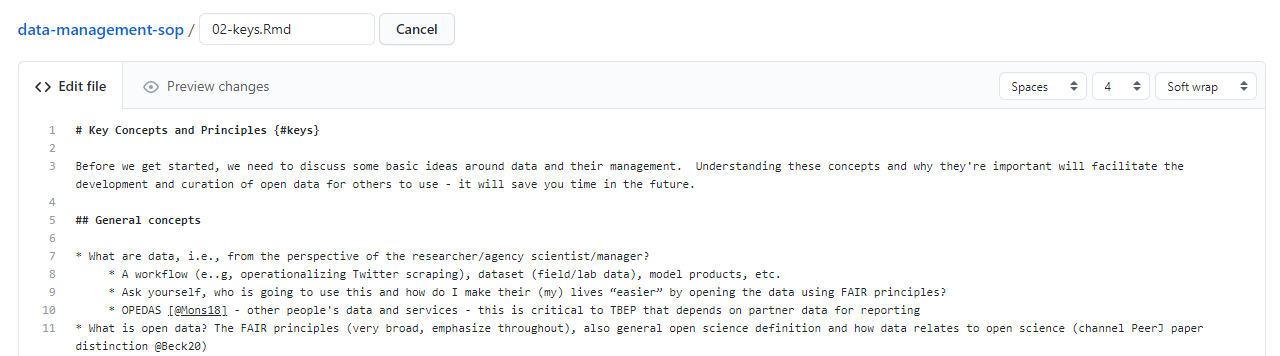
\includegraphics[width=1\linewidth]{img/editme} \end{center}

Each edit page is specific to the section where you've selected the edit button, e.g., if you click the edit button for section 2, you'll be sent to the edit page for the .Rmd file for section 2. Feel free to make any changes on the .Rmd file. When you're done, scroll to the bottom and ``commit'' your changes. This simply means you write a few words describing the edits you've made. Be as succinct as possible. When you're done, hit the green ``Commit changes'' button.

\begin{center}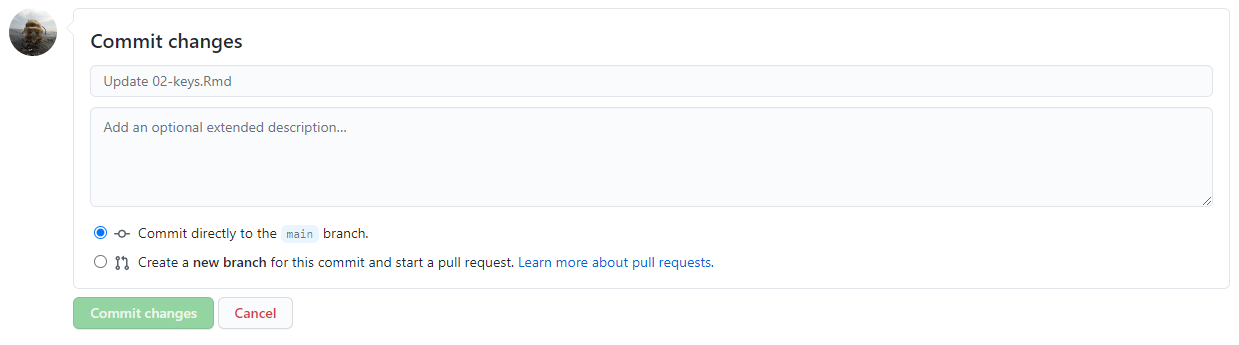
\includegraphics[width=1\linewidth]{img/editme2} \end{center}

\hypertarget{opt2}{%
\subsection{Option 2}\label{opt2}}

\emph{Requires}: Github account

Follow the above steps in \ref{opt1} by navigating to a section you'd like to edit on this website and selecting the edit button. If you don't have write access to the repository, you will see something like this:

\begin{center}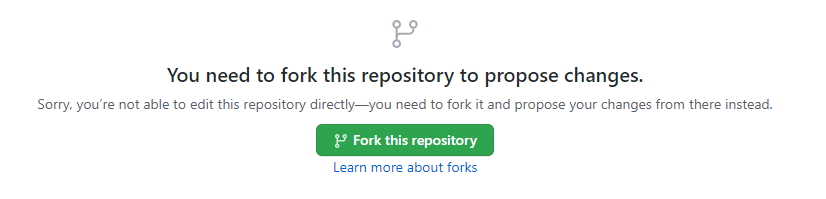
\includegraphics[width=1\linewidth]{img/editme3} \end{center}

This simply means that you need to create your own copy to edit. You can fork your own copy to your personal account and make your edits there. Once editing is done, you can submit a pull request to the original repository with your proposed changes. Not sure what this means? Check out this chapter here: \url{https://happygitwithr.com/fork-and-clone.html}

\hypertarget{opt3}{%
\subsection{Option 3}\label{opt3}}

\emph{Requires}: GitHub account

If none of the above sounds appealing, you can always post any suggestions or edits as an issue under the \href{https://github.com/tbep-tech/data-management-sop/issues}{issues tab} of the repository. When you create a new issue by clicking the giant green ``New issue'' button, you'll see something like this:

\begin{center}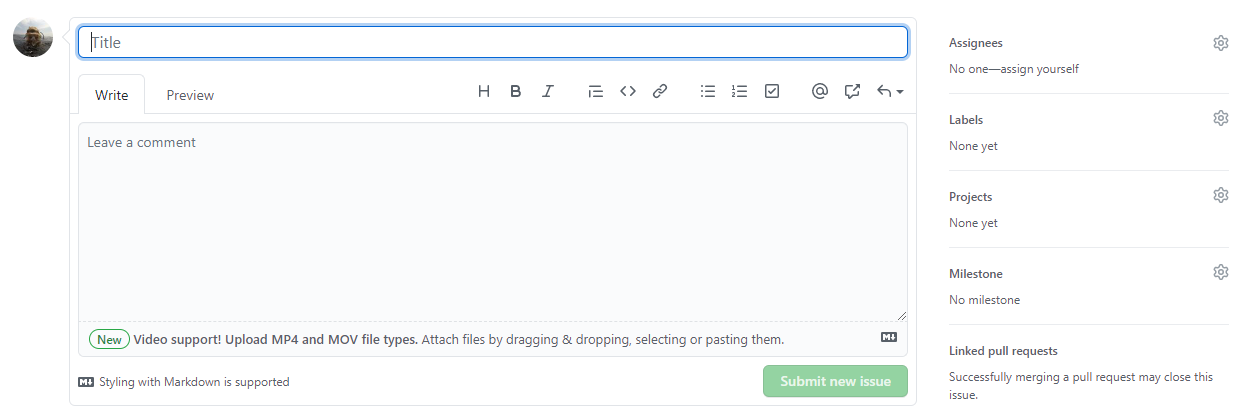
\includegraphics[width=1\linewidth]{img/issues} \end{center}

Give your issue a short but informative title (e.g., ``suggests edits to section 2''). Under the ``Write'' tab, explain what edits or changes you'd like to see. Feel free to select a member of the TBEP staff to assign the issue using the menu on the right. The issues descriptions support Markdown syntax, so get creative in your descriptions (i.e., make lists, link to documents, etc., see the \href{https://rstudio.com/wp-content/uploads/2015/03/rmarkdown-reference.pdf}{cheatsheet}).

In general, one issue should cover only one suggested change to the document. However, multiple text edits to the same document can be submitted to the same issue so long as they cover similar topics, e.g., one issue for several suggested edits to one section.

\hypertarget{opt4}{%
\subsection{Option 4}\label{opt4}}

\emph{Requires}: Email

Just \href{mailto:mbeck@tbep.org}{email me} any changes you'd like to see!

\hypertarget{about}{%
\section{About}\label{about}}

The Tampa Bay Estuary Program is one of \href{http://nationalestuaries.org/}{28 National Estuary Programs} designated by Congress to restore and protect ``estuaries of national significance.'' Administered by the U.S Environmental Protection Agency under the Clean Water Act, each program must develop a science-based plan using community input to protect and enhance the natural resources of its respective estuary and surrounding watershed.

The \href{http://ccmp.tbep.org/}{Comprehensive Conservation and Management Plan} (CCMP, updated in 2017) presents 39 actions to sustain progress in bay restoration through the year 2027. To address the actions in our CCMP, our \href{https://drive.google.com/file/d/11xohuoaHDxNHRqgXoOHdI37FpWvac_rn/view}{2021-2025 Strategic Plan} provides a framework to guide decisions about how to align personnel and financial resources with the Program's mission in ways that maximize our impact on Tampa Bay recovery. A cornerstone strategy of this plan is the use of open science principles and methods to allow the TBEP to be the primary source of trusted, unbiased, and actionable science for the Tampa Bay Estuary. This document is a reflection of these strategies.

Please visit our website for additional information about our program: \url{https://www.tbep.org}

\begin{center}\rule{0.5\linewidth}{0.5pt}\end{center}

~~This book is licensed under a Creative Commons Attribution 4.0 International License.

This version of the book was built automatically with \href{https://github.com/tbep-tech/data-management-sop/actions}{GitHub Actions} on 2021-04-27.

\hypertarget{background}{%
\chapter{Background}\label{background}}

\hypertarget{dataimp}{%
\section{Importance of data}\label{dataimp}}

Data are critical to making informed policies and decisions about how we manage behaviors and actions that affect the environment. As a fundamental part of the scientific method, data provide the raw information to support hypotheses that inform our understanding of natural processes. Data are the foundation for environmental research which develops this understanding to support informed decisions for managing natural resources. As methods for managing environmental resources continue to evolve, so does our understanding of data and its potential applications.

When we discuss ``data'' we often describe a very general term that has different meanings for different people. In its simplest form, data can be tabular information for the results of an experimental analysis or field survey. For environmental managers, data can mean the long-term record of routinely collected and updated monitoring information used to assess status and trends of a natural resource. Even further, data can be highly aggregated and novel products created through complex meta-analyses of independent datasets. In all cases, the need to describe a dataset's purpose and origin, and identify its permanent and long-term home are critical to ensure forward progress in both conventional research and how research informs environmental management.

This Data Management Standard Operating Procedure (SOP) describes TBEP's approach to address data management needs for the long-term restoration and protection of natural resources in Tampa Bay and its watershed. We are inclusive of multiple definitions of data from simple spreadsheets to more complicated workflows that generate reporting products to support environmental decisions. This broad net is designed to account for both the variety of data we use as a Program and the diversity of partner agencies we depend on to achieve our mission. The management of environmental resources combines a healthy mix of conventional science with consensus driven decisions, often with strong regulatory overtones. A robust approach for working with data that promotes trust and validity in the environmental decision and to ensure the science continues to progress without reinventing the wheel is foundational for these processes.

\hypertarget{whymanage}{%
\section{Why we need to effectively manage data}\label{whymanage}}

There are many reasons why data may not be effectively managed, chief among which is that it can be tedious and unglamorous work that is often an afterthought. However, investing time upfront to manage a dataset can have long term benefits, although these values may not be obvious or realized in the short-term. Lack of effective data management often results in ``orphaned'' datasets and data products which have lost critical reference documentation.

A classic graphic in Michener et al.~\citep{Michener97} demonstrates how knowledge of a data product can be lost over time (Figure \ref{fig:michener}). As a research team publishes a paper, the information content of the data and metadata is at an all-time high because the ideas and concepts have been intensely studied and evaluated in the months leading up to publication. After publication, researchers move on to other projects or responsibilities, and specific details about the initial project are lost rapidly as attention is focused elsewhere. At longer time scales, other factors can contribute to the erosion of information content, including career changes through retirement or staff turnover or accidental loss of information (laptop takes a bath, lab fires, etc.).

\begin{figure}

{\centering 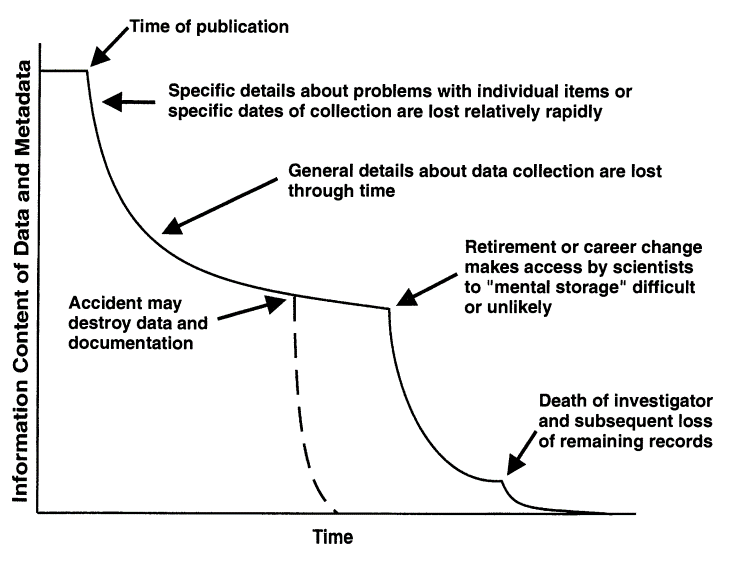
\includegraphics[width=1\linewidth]{img/michener} 

}

\caption{Loss of information over time in the absence of data management [@Michener97]}\label{fig:michener}
\end{figure}

The final step in Figure \ref{fig:michener} leading to absolute and complete loss of information on a data product is death of an investigator. Although a bit morbid, this is a very real and preventable problem in the process of discovery that can lead you down the frustrating path of reconstructing a data product's origin by scouring historical records that have little to no descriptive information. As a remedy, many research teams have adopted the ``bus factor'' term as motivation to prevent this problem. The bus factor is an informal measurement of the relative risk associated with loss of information if an investigator was to, hypothetically, be hit by a bus (alternatively, the ``lottery factor'' describes departure of an individual if they were to win the lottery). Datasets or workflows that have a high bus/lottery factor are at high risk of being orphaned with the departure of a team member.

The costs of not effectively managing your data can vary, but each is a byproduct of neglecting an investment in data curation. In fact, you can probably recall several past instances when poor data management has come back to haunt you. Here are a few real-world examples:

\begin{enumerate}
\def\labelenumi{\arabic{enumi})}
\tightlist
\item
  A collaborator calls you on the phone asking about a historical dataset from an old report. You spend several hours tracking down this information because you don't know where it is. The data you eventually find and provide to your collaborator has no documentation and they don't know how to use it or use it inappropriately.
\item
  You receive a deliverable from a project partner that was stipulated in a scope of work. This deliverable comes in multiple formats with no reproducible workflow to recreate the datasets. You are unable to verify the information, eroding your faith in the final product and making it impossible to update the results in the future.
\item
  An annual reporting product requires using new data each year. The staff member in charge of this report spends several days gathering the new data and combining it with the historical data. Other projects are on hold until this report is updated. Stakeholders using this report to make decisions do not trust or misunderstand the product because the steps for its creation are opaque.
\end{enumerate}

A more general problem with poor data management is stifled creativity. The use of other people's data and services \citep[i.e., ``OPEDAS'';][]{Mons18} to generate novel research or data products is increasingly common, particularly in the last twenty plus years with the advance of internet communications. Entire disciplines and new analytical methods have been developed around this idea \citep[e.g., meta-analysis;][]{Carpenter09, Lortie14}. The generation of new data with an incomplete history or that lack metadata documentation is a disservice to both the researcher that created the data and the larger scientific community that could benefit from using this information. As a result, scientific progress will not continue as rapidly as it could if data products are discoverable and openly available.

Poor data management can also lead to peculiar or entrenched workflows that are not scalable or translatable for other users. Data managers often have their own preferences for processes that simply ``work for us'', either because they were learned out of necessity because the work had to be done or it has been done a certain way for so long that it now seems normal, despite being inefficient or prone to error. In extreme cases, this can lead to workflows that may seem legitimate on the surface but are problematic because they lack a common formality or standards.

\citet{Mons18} describes ``professorware'' as a workflow to handle or generate data that addresses a novel intellectual challenge, which is important in research or discovery, but is not scalable or sustainable in the long run. Think of a pet project where you've written some code to achieve a certain task. It might be clunky, but you're proud of it because it gets the job done on your computer and saves you from having to do a task by hand. These workflows often masquerade as novel ``software packages'' that do great things, which they can and often do, but they lack support because they're not developed using community standards or best practices for long-term use or scalability. This is especially problematic when these workflows are intentionally or unintentionally embedded into larger data management systems. If one piece of the system lacks provenance or support, it puts the larger data management system at risk.

In summary, poor data management practices can lead to the following:

\begin{itemize}
\tightlist
\item
  Less collaboration in the research community
\item
  Increased siloing among management institutions
\item
  Less creative approaches to managing environmental resources
\item
  Inefficient and error prone workflows that are neither scalable nor sustainable
\end{itemize}

\hypertarget{opengeneral}{%
\section{Open Science}\label{opengeneral}}

The open science approach provides a philohy and set of tools to help address the costs of poor data management. Before we proceed, we need to make a distinction between the broader concept of open science and open data as one component of the former. Many of the guidelines and examples in this SOP fall broadly under the open science umbrella (or cake as you'll see in section \ref{philo}), but it's important to understand how data management includes a set of tools that are part of, but not exhaustive of, the entire open science toolbox. Conversely, many broadly applicable open science tools that can be applied to other management scenarios can also benefit data management.

An example may be helpful. Metadata, a key component of data management, leads to more open sharing. When we talk about metadata, the assumption is that its creation is to promote sharing and transparency for open data. However, while metadata can be created in an open environment and is often created for the purpose of facilitating openness, it can also be created completely in isolation with a closed workflow, resulting in a significant potential for loss of important information.

On the other hand, broader open science principles that support a culture of sharing can also have value for research workflows that generally have nothing to do with data. For example, the ``public school of thought'' for open science focuses on making science more accessible to the general public, e.g., through citizen science initiatives or science blogging \citep{Fecher14}. Although this approach doesn't deal explicitly with best practices for data management, this mentality certainly has benefit for creating a culture that appreciates and learns from science, which logically leads to discussions on the importance of data.

For these reasons, this document covers many topics that may fall squarely under the realm of data management, while at other times advocating for more general open science principles with the intent of supporting a culture of better data management.

\hypertarget{philogeneral}{%
\section{The TBEP philosophy}\label{philogeneral}}

The Tampa Bay Estuary Program (\href{https://www.tbep.org}{TBEP}) is one of \href{http://nationalestuaries.org/}{28 National Estuary Programs} designated by Congress to restore and protect ``estuaries of national significance.'' Many of these estuaries are heavily urban (i.e., having economic, recreational, cultural importance) and have had historical or ongoing issues contributing to poor environmental quality. The recovery of Tampa Bay is an exceptional story of an urban estuary that demonstrates the value of the NEP approach to restoring and protecting environmental resources. Through a coordinated regional effort of environmental professionals, utility operators, community members, and local politicians, nutrient loads to the bay have been reduced by \textasciitilde2⁄3 from 1970s levels and seagrasses surpassed the 1950s benchmark extent in 2014 \citep{Greening14, Sherwood17}. Even more remarkable is that while the human population in the Tampa Bay watershed continues to increase, nutrient loads into the Bay remain low.

The TBEP is a key facilitator among the many local partners that have an interest in the region's natural resources. Our facilitation is guided by several documents, including an \href{https://drive.google.com/file/d/1iJcWxmc5SeyDTqiCQ3MLQGWEY_EDGtZT/view?usp=sharing}{Interlocal Agreement} with our partners, a \href{https://indd.adobe.com/view/cf7b3c48-d2b2-4713-921c-c2a0d4466632}{Comprehensive Conservation and Management Plan}, and a \href{https://drive.google.com/file/d/11xohuoaHDxNHRqgXoOHdI37FpWvac_rn/view?usp=sharing}{Strategic Plan}. In simple terms, these documents respectively describe \emph{who} we work with, \emph{what} we need to accomplish, and \emph{how} it can be accomplished.

Open science and data management have everything to do with how we facilitate bay management. Our recent update to the Strategic Plan specifically speaks to our use of open science as 1) a general direction for how we accomplish our work to achieve the desired future state of Tampa Bay and 2) as a unique value proposition that TBEP offers within its sphere of influence. We articulate the use of open science at TBEP as a cornerstone strategy:

\begin{quote}
Be the primary source of trusted, unbiased, and actionable science for the Tampa Bay estuary, recognizing that open science principles will serve the Program's core values.
\end{quote}

As a Program with a small staff, successful protection of Tampa Bay's natural resources depends on the work of our many partners. While we use open science principles internally, we can have a much greater impact if our partners understand the value of open science and actively work towards adopting its principles in their own workflows. We are actively supporting our partners through this journey through an Open Science Subcommittee that has a goal of developing a community of practice that works and learns together to navigate the open science landscape. Our \href{https://docs.google.com/document/d/1w6dVTwfYYDRVzGPXy0jyHxV4mwOutEY_ISMP1oAdZ_c/edit}{roles and responsibilities} document explains how we are accomplishing this goal.

Our Program rests on a strong foundation of \href{https://tbep.org/our-work/library/}{research} that guides decision-making for Tampa Bay covering three decades of science and collaboration. Although great strides have been made, we intend to continue building on those accomplishments as an organization, including enhanced data management practices guided by open science principles. The details of this approach and why we've adopted open science as our own are explained fully in section \ref{philo}.

\hypertarget{goals-and-objectives-of-this-document}{%
\section{Goals and objectives of this document}\label{goals-and-objectives-of-this-document}}

The overarching goal of this document is to achieve the following:

\begin{quote}
Motivate internal staff and external partners to become stewards of their data by demonstrating the value of open data practices and providing a road map to achieving this goal.
\end{quote}

Each section of the SOP addresses a critical topic or provides a roadmap that collectively helps us work towards achieving this goal. The sections are as follows:

\begin{itemize}
\tightlist
\item
  Section \ref{keys}: An overview of general and specific topics that are useful to understand for data management
\item
  Section \ref{workflow}: An explanation of how TBEP manages data and a roadmap to developing your own workflows
\item
  Section \ref{cases}: Examples describing specific projects and why/how data management practices were applied to each
\item
  Section \ref{final}: Parting thoughts and words of wisdom to help you continue on your open science and data management journey
\item
  Section \ref{appendices}: Definitions and resources for continued learning
\end{itemize}

The TBEP has also developed a data \href{https://drive.google.com/file/d/1DyA0PNHV8rEXGMwGiyS7sXY1ECLYpJJO/view}{Quality Management Plan} \citep[QMP;][]{tbep1620}. This SOP and the QMP can be viewed as partner documents that complement each other, but are developed to meet different needs. The goal of this SOP is described above. The goal of the QMP is to ensure the data used by TBEP for decision-making has known and documented quality and is being used appropriately. In other words, the QMP establishes an internal process for ensuring data quality conforms with federal or grant-reporting requirements, whereas this document is a generalized introduction and how-to approach for data management that can help us achieve goals of the QMP.

Identifying what this SOP is and what it is not can help us set expectations for this document. As noted above, the TBEP is a relatively small organization with hands in many projects supported or managed primarily by our partners. Because of the diversity of projects relevant to our work, it would be inappropriate and impossible to describe a detailed step-by-step SOP that could apply to every project. Therefore, the approach and workflows we describe are meant to be generalizable to many project types. Any specificity that is described relates to how to use tools that have broad applicability, e.g., developing a GitHub workflow or describing general characteristics of metadata that could apply to many data types. This distinguishes this SOP from others that may apply rigorous standards to one particular problem.

To summarize, this document \textbf{is}:

\begin{itemize}
\tightlist
\item
  An explanation of the TBEP approach to data management, including our philosophy and the existing tools we have developed
\item
  A generalized cookbook describing how to manage datasets in an open science framework, including considerations before, during, and after a project
\end{itemize}

This document \textbf{is not}:

\begin{itemize}
\tightlist
\item
  A definitive overview of best practices for data management; there are other resources (see section \ref{appendices}) that cover these topics in more detail
\item
  A comprehensive list of available online services for opening data, although we certainly lean towards specific platforms that we find useful
\end{itemize}

Finally, the intended audience for this SOP is TBEP internal staff and our external partners. In both cases, the text is written to target technical staff, although the concepts and principles are appropriate for some tasks conducted by managers or higher administrative staff. These individuals are also in a position to foster better practices for data management by creating space and time for technical staff to adopt these new workflows. Understanding the importance of the tools is important, but sufficient space must be available for these skillsets to grow through a shared community of practice. Over time, the return on investment in creating a space for these skillsets to develop will be realized.

\hypertarget{keys}{%
\chapter{Key Concepts and Principles}\label{keys}}

Before we get started, we need to discuss some basic ideas around data and their management. Understanding these concepts and why they're important will facilitate the development and curation of open data for both you and others to use. Some of these concepts are very general, whereas others may seem fairly specific. The detailed concepts may seem daunting, but they are critical in supporting your journey in managing your own data.

\hypertarget{contribs}{%
\section{Identifying important contributions}\label{contribs}}

We briefly introduced a general concept of data in section \ref{dataimp}. Throughout this document, we use the term ``data'' to describe a variety of products either directly supporting decision-making processes or used for research to support the former. Data can be generated to support or refute hypotheses in research, whereas research can also produce data products that support environmental management. The end game in all of these processes is understanding that data can be present at any stage in research and/or decisions that support environmental management. As a results, individuals may use ``data'' to describe products at any point in this workflow. Understanding the different ways we talk about data will allow you to more carefully identify your data management needs.

Identifying the types of data that are important to support decision-making is the first task in developing a data management workflow. Any research project could produce countless datasets and it may be challenging to understand which datasets are important or are merely intermediate steps in a larger process. To help you identify which datasets are important to your project, ask these questions:

\begin{enumerate}
\def\labelenumi{\arabic{enumi}.}
\tightlist
\item
  What is the most important and tangible contribution of this project?\\
\item
  Who is going to benefit from the results of this project?
\item
  How can I use data management practices to make the use of these data ``easier'' for decision-making?
\end{enumerate}

Answers to these questions can help you identify important data products for developing data management workflows. However, identifying the single most important dataset is challenging and a typical answer to what is the greatest data contribution for a project usually is ``it depends''. Also realize that you may be the direct beneficiary of a particular research project - documenting and using proper data management workflows will save you from headaches in the future. Evaluating these questions at different steps throughout a project can help you identify the valuable contributions.

In a perfect world where we have endless time and resources, and not to mention interest, to dedicate to data management, we would track and document the provenance of every single dataset used by a research project. Of course, this is not practical, nor do we need to curate every piece of data. You will need to identify the most important contribution of a project among alternatives based on your answers to the above questions. Here are a couple scenarios that can help in this process.

\begin{quote}
I am collecting field data and/or running experiments in a laboratory.
\end{quote}

The field or experimental data are obvious candidates for developing a data management workflow, yet it is rarely a solitary dataset that is produced. Working with these data continuously throughout a project will benefit from developing a data dictionary (section \ref{dict}) and understanding linking keys between different data tables. If you don't want or need to archive all the datasets you've used or created, identify a master dataset that provides the main results for your study.

\begin{quote}
I am using data from an external source as primary or secondary information to support analysis or generate a reporting product
\end{quote}

A derived dataset may be the most important contribution of this project. This dataset can include multiple combinations of input datasets from external sources. It is important to document the steps that were used to develop this dataset, including the raw sources of information and where they can be accessed. Documentation can range from a general description of the dataset (less desirable) to complete access to source code for reproducing the derived dataset (more desirable). The most important contribution may be the workflow or the derived dataset, depending on ``who'' can benefit most from this project.

\begin{quote}
I am producing a model to support scenario exploration or understanding of natural processes
\end{quote}

Tracking data provenance of a modelling project is a challenging task simply because a ``model'' does not conform to the conventional understanding of data. As noted above, we describe data as anything that can support decision-making in environmental management. Models are commonly used for this task, yet understanding of their information content over time often rests with one individual, giving that modeller a very high bus factor. There are practical limitations for fully tracking a model as a data product (e.g., computational limits, time requirements, required knowledge of its working components), but there are certainly derived datasets from models that can benefit from data management. In particular, model results, parameters, or source code are all prime candidates for data management, depending on the audience.

\begin{quote}
I am developing a decision-support tool
\end{quote}

Related to the challenges of data management for modelling, so-called ``decision-support'' tools are increasingly used as a front-end for decision-makers to access relevant information from a research project or intensive data collection effort. Online interactive dashboards have proliferated tremendously in the last ten years to meet this need. These tools can be useful in the right hands, yet there is no community standard for how to treat these products as data to track their origin and metadata. In this case, documenting the workflow, source code, and requisite datasets for powering the dashboard may be the most important contributions. \href{https://journals.plos.org/ploscompbiol/article?id=10.1371/journal.pcbi.1003542\#s4}{Rule 4} under the ten simple rules for the ``care and feeding'' of scientific data \citep{Goodman14} describes publishing workflows as important context.

In summary, identifying the most important data contribution is a challenge that can guided through careful evaluation of the above. This may lead you to choose one or more data products to develop a data management workflow for a specific project. These could include:

\begin{itemize}
\tightlist
\item
  Tabular data either as standalone or as several tables linked by common keys
\item
  Derived or synthesis data, often tabular, created as the sum of other, disparate datasets
\item
  Model output or model information that describe environmental processes or likely outcomes of management scenarios
\item
  Workflows to creating a data product, which could include analysis code as a continuous pipeline from source to product
\item
  An online dashboard to support user engagement with data
\end{itemize}

\hypertarget{fair}{%
\section{The FAIR principles}\label{fair}}

The previous section presented several questions to ask yourself that can aid in identifying important contributions of a research project as a focus for data management. In all cases, once that important contribution is identified, community standards or best practices for that dataset or product should be used to ensure the intended audience can find, access, use, and replicate the data. The FAIR principles \citep{Wilkinson16} provide some general guidelines to follow for ensuring the openness of a data product. The FAIR acronym is described as follows:

\begin{itemize}
\tightlist
\item
  \textbf{F}indable: The data have a globally unique and persistent identifier, including use of ``rich'' metadata.
\item
  \textbf{A}ccessible: Once found, the data can be retrieved using standardized communications protocols that are open, free, and universally implementable.
\item
  \textbf{I}nteroperable: The ability of data or tools from non-cooperating resources to integrate or work together with minimal effort.
\item
  \textbf{R}eusable: If the above are achieved, the data and metadata are described in a way that they can be replicated and/or combined in different settings.
\end{itemize}

What this means simply is that 1) each dataset has a name that doesn't change and can be found with minimal effort using that name, 2) once it's found, you can actually get your hands on it (e.g., not behind a paywall), 3) once you have it, you can use readily available tools to work with the data (e.g., not using proprietary software), and 4) you can actually apply the data for your own needs because it has sufficient context, including its reproduction, given the the first three principles are met.

In practice, the FAIR principles invoke several concepts that will be described in detail later, but we describe some here as a gentle introduction. The term ``globally unique and persistent identifier'' (under \textbf{F}) is a mouthful that simply means the dataset has a name assigned to itself that is not assigned to any other dataset (globally unique) and it's permanent (persistent). This doesn't mean a descriptive or literal name, such as you would assign to a file on your own computer, rather it means a computer-generated identifier created using a known standard. One such example is a \href{https://www.doi.org/}{DOI}, or digital object identifier. These are commonly assigned to publications as a static web address (unique and persistent) and are increasingly being used as identifiers for datasets.

Findable and accessible also imply the data have a home with an address. The latter describes the unique identifier, whereas the home itself is permanent location as a requirement for accessibility. There are several options for where data can live long-term and theoretically forever so long as the internet exists. There are literally thousands of repositories online that can be used for archiving data and the answer to which repository you should use is also almost always going to be ``it depends''. We provide some examples in section \ref{moregit} as one option used by TBEP.

The FAIR principles are not rigorous standards, rather they establish general questions you should ask of a dataset to make sure you've done your due diligence in working towards openness. Further, because they are not rigorously defined, different organizations may interpret the principles differently and it's important to realize that your understanding of the principles may differ from others. For example, individuals may define ``reusable'' in different ways that can affect the level of detail provided in the metadata. These principles are presented here as a reminder to think about them often, especially during the beginning of a project, and how they can be applied in opening the most important contribution of your project.

\hypertarget{whytidy}{%
\section{The importance of tidy data}\label{whytidy}}

We introduced different data products in section \ref{contrib} ranging from tabular data to more abstract definitions that may include analysis pipelines or online services. Tabular data are by far the most recognized and most common data type and it's worth covering a few basic principles for managing these data that will help you tremendously in the long run. At their core, tabular data are a simple conceptual model for storing information as observations in rows and variables in columns, yet its very common to try to make a table more than it should be. Unless you spend a lot of time working with data, it can be difficult to recognize common mistakes that lead to ``table abuse''.

Before we get into tidy data, we need to discuss some of the downfalls of Excel as a data management system. There are \href{http://www.eusprig.org/horror-stories.htm}{many examples} that demonstrate how Excel has contributed to costly mistakes through the abuse of tables, often to the detriment of science \citep{Ziemann16}. Although it is a very interesting and clever program, it is not software developed for data storage. It is a graphical user interface masquerading as data management and analysis software. It includes many tools that may appear useful for organizing information, but that ultimately increase risk and make your life as an analyst more difficult.

Excel allows you to abuse your data in many ways, such as adding color to cells, embedding formulas, and automatically formatting cell types (figure \ref{fig:excelbad}). The problem occurs when this organization becomes ambiguous and only has meaning inside the head of the person who created the spreadsheet. For example, color may be used to fill cells of a given category. This may seem harmless, but in doing so, you've not only indirectly created more data, but you've created data that have an ambiguous meaning. Embedding formulas that reference specific locations in or across spreadsheets is also a nightmare scenario for reproducibility. There is no clear way to extract the hidden workflow embedded in many spreadsheets.

\begin{figure}

{\centering 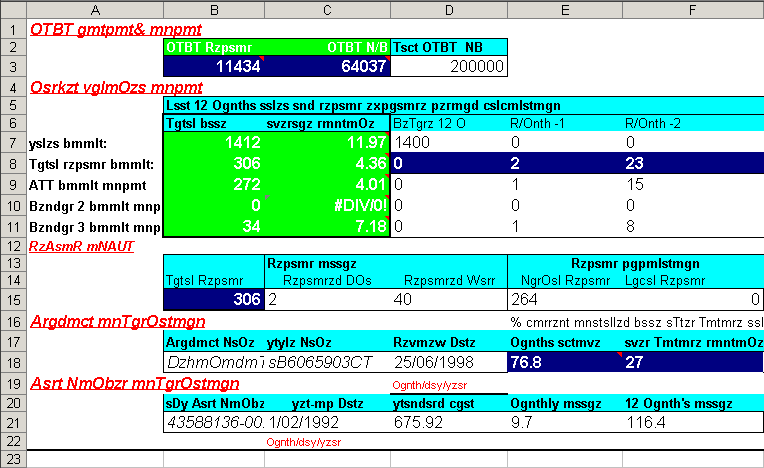
\includegraphics[width=0.8\linewidth]{img/excel_bad} 

}

\caption{An exceptional example of table abuse using Excel.}\label{fig:excelbad}
\end{figure}

If you absolutely must use Excel to store data, the only acceptable format you should use as a responsible data steward is a rectangular, flat file. We mean ``rectangular'' as storing data only in rows and columns in matrix format (e.g., 10 rows x 5 columns), with no ``dangling'' cells that have values outside of the grid or more than one table in a spreadsheet. We mean ``flat file'' as no cell formatting, no embedded formulas, no multiple spreadsheets in the same file, and data entered only as alphanumeric characters. This will ensure that there is no ambiguous information and a machine will have no problem reading your spreadsheet. Your data will be pure and simple and not abused. \citet{Broman18} provide an excellent guide that expands on these ideas. Essentially, these best practices force you to isolate the analysis from the data - many people use Excel to mix the two, leading to problems.

Now we can introduce some additional principles for tabular data that will improve how they are used in downstream analysis pipelines. The ``tidy'' data principles developed by Hadley Wickham \citep{Wickham14c} are a set of simple rules for storing tabular data that have motivated the development of the wildly popular tidyverse suite of R packages \citep{Wickham19}. If you're already using the rectangular, flat file format, adopting the tidy principles should be a breeze. The rules are simple:

\begin{enumerate}
\def\labelenumi{\arabic{enumi}.}
\tightlist
\item
  Each variable must have its own column
\item
  Each observation must have its own row
\item
  Each value must have its own cell
\end{enumerate}

Graphically, these rules are shown in figure \ref{fig:tidy}.

\begin{figure}

{\centering 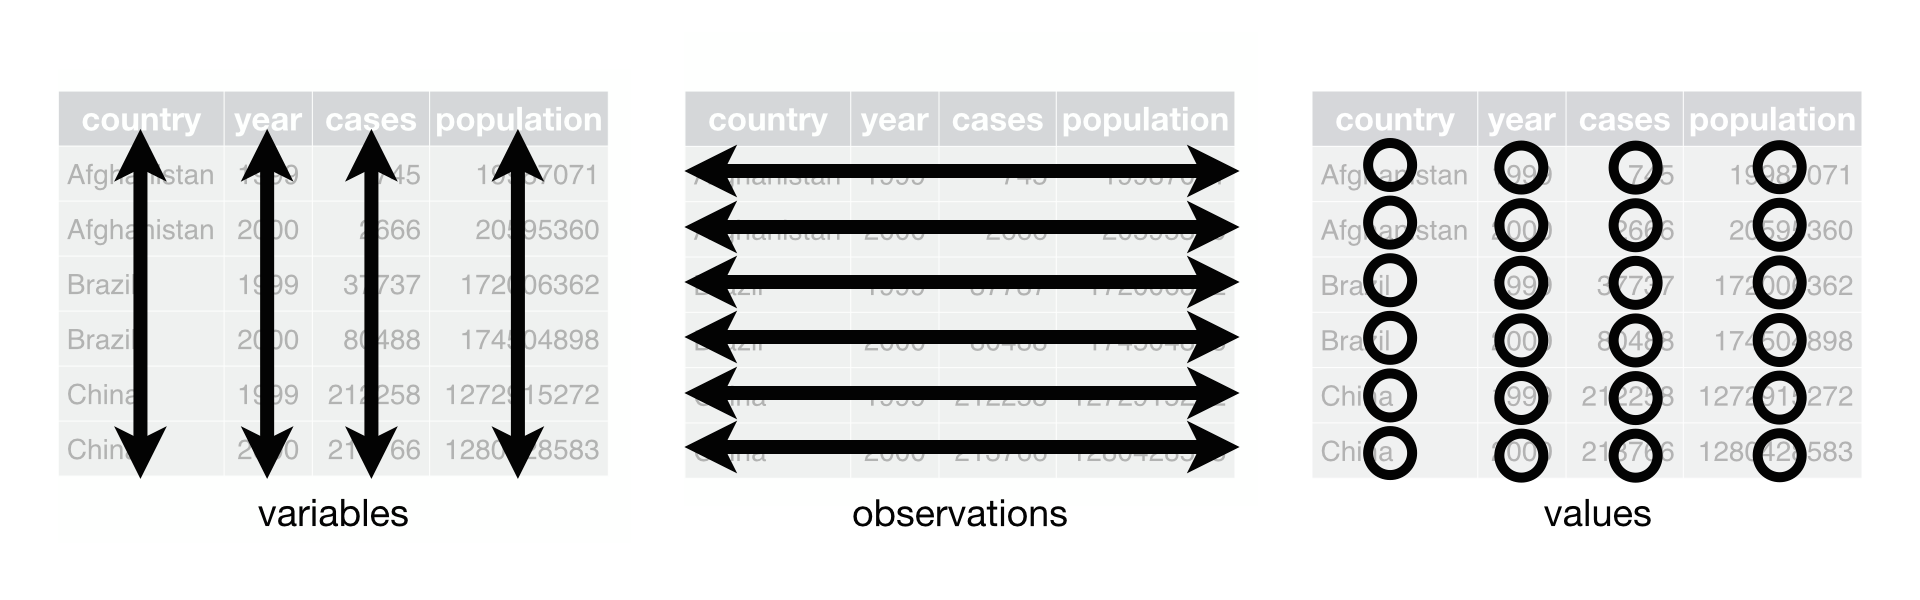
\includegraphics[width=1\linewidth]{img/tidy-1} 

}

\caption{A representation of the rules for tidy data (from @Wickham17).}\label{fig:tidy}
\end{figure}

Using these principles for data storage may seem unnatural at first because of a difference between what's easy for entering data versus what makes sense for downstream analyses. The former is what leads to abuse of tables. For example, dates are often spread across multiple columns, such as having one column for each year of data where the header indicates the year that applies to data in each column. This convention may be used because it's easy to add another year of data as an additional column when more data each year are collected. However, this is untidy because the date variable occurs across columns. If you wanted to evaluate changes across years in a formal analysis, you'd have to reorganize these data in a tidy format.

Using a tidy format also allows you to more easily merge or join data between tables. This is a common task when analyzing data where you have information spread between different tables because 1) it might not make sense to keep the data in a the same table and 2) the analysis depends on information from both tables. For example, perhaps you want to evaluate how a measured variable at different locations changes across space. You might have one table that includes station metadata (e.g., site name, location) and another table that includes field observations (e.g., site name, collection date, field data) (Figure \ref{fig:joins}). Keeping the station metadata in a tidy format in one table makes sense because these data will not change. Keeping field data in another table would also make sense because you collect information at each location at different times. Including station coordinate information in the same table as the field data would create extra information because you need a value for location for every row you have field data. This is redundant and unnecessary.

If you're using a tidy format, it's simple to join two tables for analysis. This requires identifying a linking variable or ``key'' that is a common identifier between tables. In the above example, this would be the site name (Figure \ref{fig:joins}). Other situations may require identifying more complex keys depending on your analysis question. Our question above related to evaluating station differences by location, so the site name is a logical choice for a key. For all cases, a key is used to resolve a uniquely identifiable value that can be used to link observations. A more involved example is provided in section \ref{oyster}. If the important data contribution of your project includes multiple tables, you'll need to identify appropriate keys that allow you to link observations between tables.

\begin{figure}

{\centering 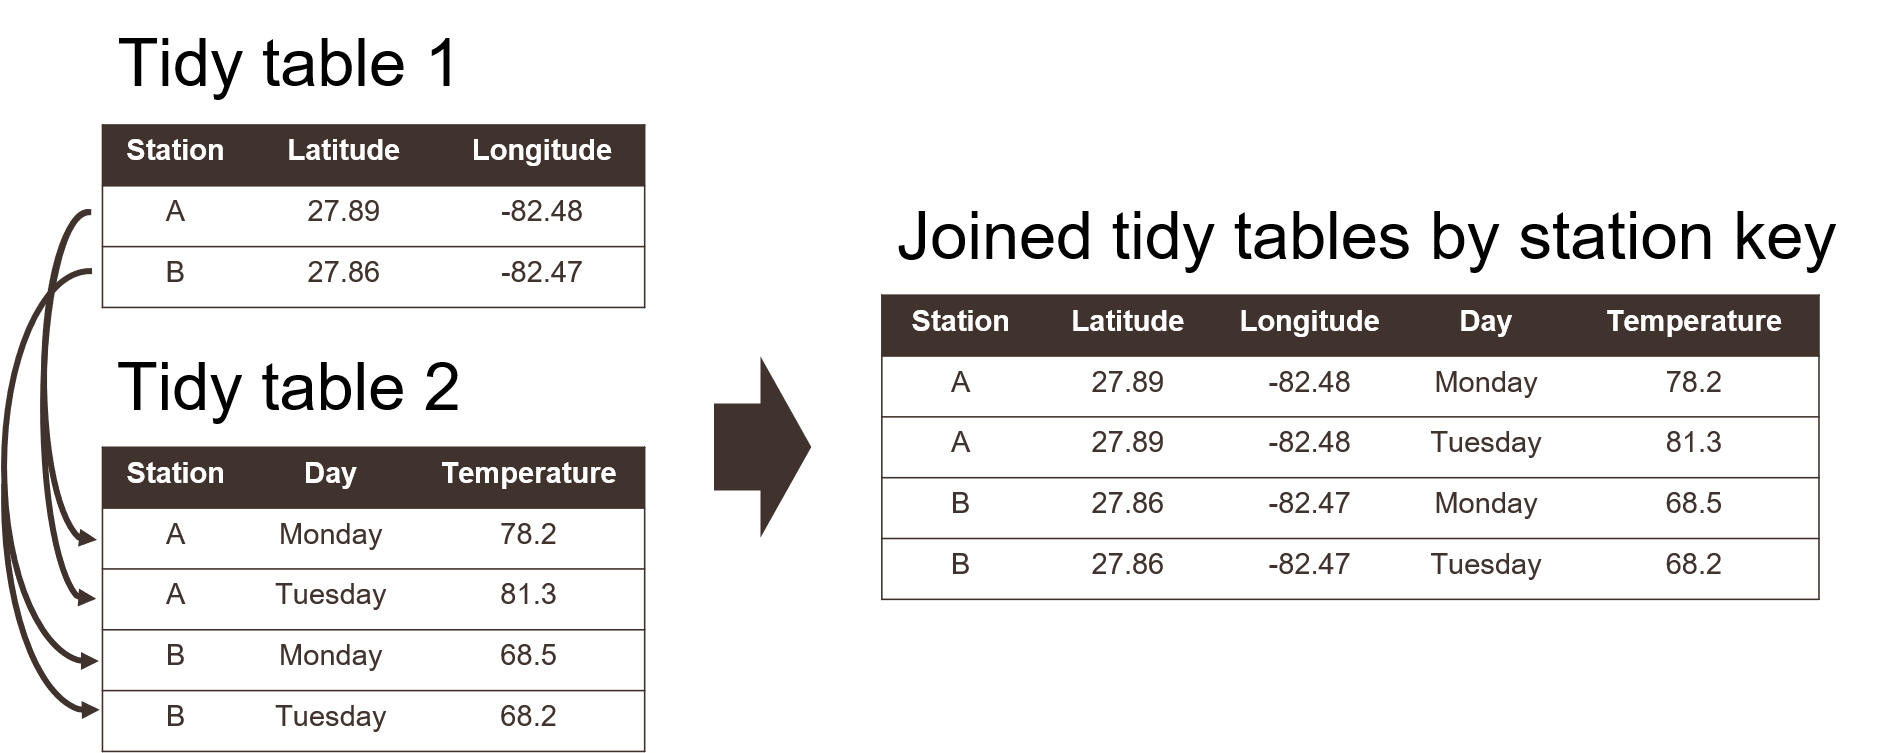
\includegraphics[width=1\linewidth]{img/joins} 

}

\caption{Joining two tidy tables by a shared key.}\label{fig:joins}
\end{figure}

\hypertarget{metadatadesc}{%
\section{Metadata}\label{metadatadesc}}

Just as ``data'' can have different meanings to different people, ``metadata'' is a loosely defined term that describes one of the most important aspects of data management. Metadata varies from simple text descriptions of a dataset, such as ``who'', ``what'', ``when'', ``where'', ``why'', and ``how'', to more formalized standards with the intent of preparing your data for archival in a long-term repository. Having no metadata is almost a guarantee that your dataset will be orphaned or misused by others, either inadvertently or with willful acknowledgment that the original purpose of the data is unknown and its use may be inappropriate for the task at hand. Metadata are also important for enabling discovery of your data (the \textbf{F} in FAIR). So, when you think of data management, you should think of it as synonymous with metadata curation.

Metadata is literally defined as ``data about data'' or ``information about information''. A more comprehensive definition is provided by \citet{Gilliland16}:

\begin{quote}
A suite of industry or disciplinary standards as well as additional internal and external documentation and other data necessary for the identification, representation, interoperability, technical management, performance, and use of data contained in an information system
\end{quote}

We use this definition as a starting point to develop our thinking around best practices for metadata generation and curation. Again, it's good to emphasize that some metadata is way better than no metadata at all. Just because you are not using industry or disciplinary standards for generating metadata doesn't mean you're approach is incorrect. As you get comfortable with the general purpose of metadata and how it's developed as a description for a dataset, you can build on this knowledge by working towards more formalized metadata standards.

At its basic level, think of metadata as a simple text file containing the information about your dataset. This text file provides answers to common questions about the origin of your data so that anyone (or a computer) with zero knowledge about your data can quickly orient themselves as to what the data represents and its purpose. The US Geological Survey provides a useful document on creating \href{https://prd-wret.s3.us-west-2.amazonaws.com/assets/palladium/production/atoms/files/Metadata\%20in\%20Plain\%20Language_508compliant.pdf}{Metadata in ``plain language''} to distill the basic information contained in a metadata file. As indicated above, it provides a workflow for answering the ``who'', ``what'', ``when'', ``where'', ``why'', and ``how'' questions for metadata. We provide a brief synopsis of these questions below. You can use this workflow to generate your own metadata.

\begin{quote}
What does the dataset describe?
\end{quote}

Information here would include very basic details about the dataset including a \textbf{title}, \textbf{geographic extent}, and \textbf{period of time} covered by the data. For geographic extent, this may often include explicit coordinates covering the study area, i.e., the lower left and upper right of a bounding box. Location is useful for indexing your dataset relative to others, if for example, a researcher wanted to find data for all studies in the geographic extent of Tampa Bay. Other useful information about the ``what'' might include the type of data, e.g., tabular, map, online dashboard, etc.

\begin{quote}
Who produced the dataset?
\end{quote}

This would be yourself and anyone else who has made a significant contribution to the development of a dataset. People may have differing opinions regarding what defines a ``significant'' contribution, but as the curator of a dataset, it's up to you to determine how important it is for including an individual as a contributor. Data are increasingly being used as citable resources and including individuals that were important in its generation ensures proper attribution. For scientific publications, each author is generally expected to have made substantial contributions to the study conception and design, data acquisition or analysis, or interpretation of results. The same would apply to data. If someone has spent hours toiling in the field to collect the data or hours visually scanning a spreadsheet for quality control, include them!

\begin{quote}
Why was the dataset created?
\end{quote}

Describing why a dataset was created is critically important for developing context. If others want to use your data, they need to know if its appropriate for their needs. Here you would describe the goal or objectives of the research for which the data were collected. It should be clear if there are limitations in your data defined by your goals. For example, you may have collected field data in a particular time of year to address questions about seasonal changes. Using these data to answer broader temporal questions, such as inter-annual changes, would be inappropriate and could lead to invalid conclusions if someone using your data were not aware of this limitation. Identifying the ``why'' of your dataset could also prevent misinterpretation or misuse of the data by non-specialists. Think of it as an insurance policy for your data.

\begin{quote}
How was the dataset created?
\end{quote}

Here you would describe the methods used to generate the data, e.g., field sampling techniques, laboratory methods, etc. This information is important so others can know if you've used proper and accepted methods for generating the data. Citing existing SOPs or methods that are recognized standards in your field would be appropriate. If you are generating a synthesis data product using data from external sources, make sure to document where those data come from and the methods you used for synthesis. Pay attention to documenting the software that was used, including the version numbers. If you have analysis code or script that was used for synthesis, provide a link if possible.

\begin{quote}
How reliable are the data?
\end{quote}

It's also very important to document aspects of a dataset that affect reliability. The answers you provide to the above questions can provide context to this reliability, but it's also important to explicitly note instances when the data could be questionable or inappropriate to use. Here you could describe any quality assurance or quality control (QAQC) checks that were used on the data. There are often formalized ways to do so, such as codes or descriptors in tabular data defining QAQC values (e.g., data in range, below detection, sensor out of service, etc.). You will want to clearly describe what each of these codes mean and if they cover the range of conditions possible for your data. Other QAQC procedures, such as how the data were verified for accuracy, can also be described.

\begin{quote}
How can someone get a copy of the dataset?
\end{quote}

Good metadata has information on who has the data and how to contact them for requesting access. This contact may not be the same as who created the dataset (e.g., IT staff). For archived or publicly available data, this information is more important for who to contact should someone have questions. Information on obtaining a copy of the data should also describe any special software or licensing issues related to accessing the data. Under the \textbf{I} in FAIR, you should strive to make your data as interoperable as possible and not store your data in an obscure format that requires specialized software. If this is unavoidable (e.g., your data are large and it needs to be compressed), describe what needs to be done to access the data. Any licensing or permissions issues on using data should also be described, e.g., is it free for use with or without attribution, are there limitations on its use, etc. The \href{https://r-pkgs.org/license.html}{licensing chapter} in \citet{Wickham15} is a great resource to learn more about these issues. Although this chapter relates to code licensing, the same principles could apply to data.

\hypertarget{metadata}{%
\subsection{Metadata examples}\label{metadata}}

Now that we've covered the general concepts of what is included in metadata, we provide some examples of what this looks like in practice. At it's simplest, metadata can be a text file that includes information on the questions above. Below is one such example of metadata that accompanies a dataset that we describe in section \ref{desoto}.

\begin{figure}

{\centering 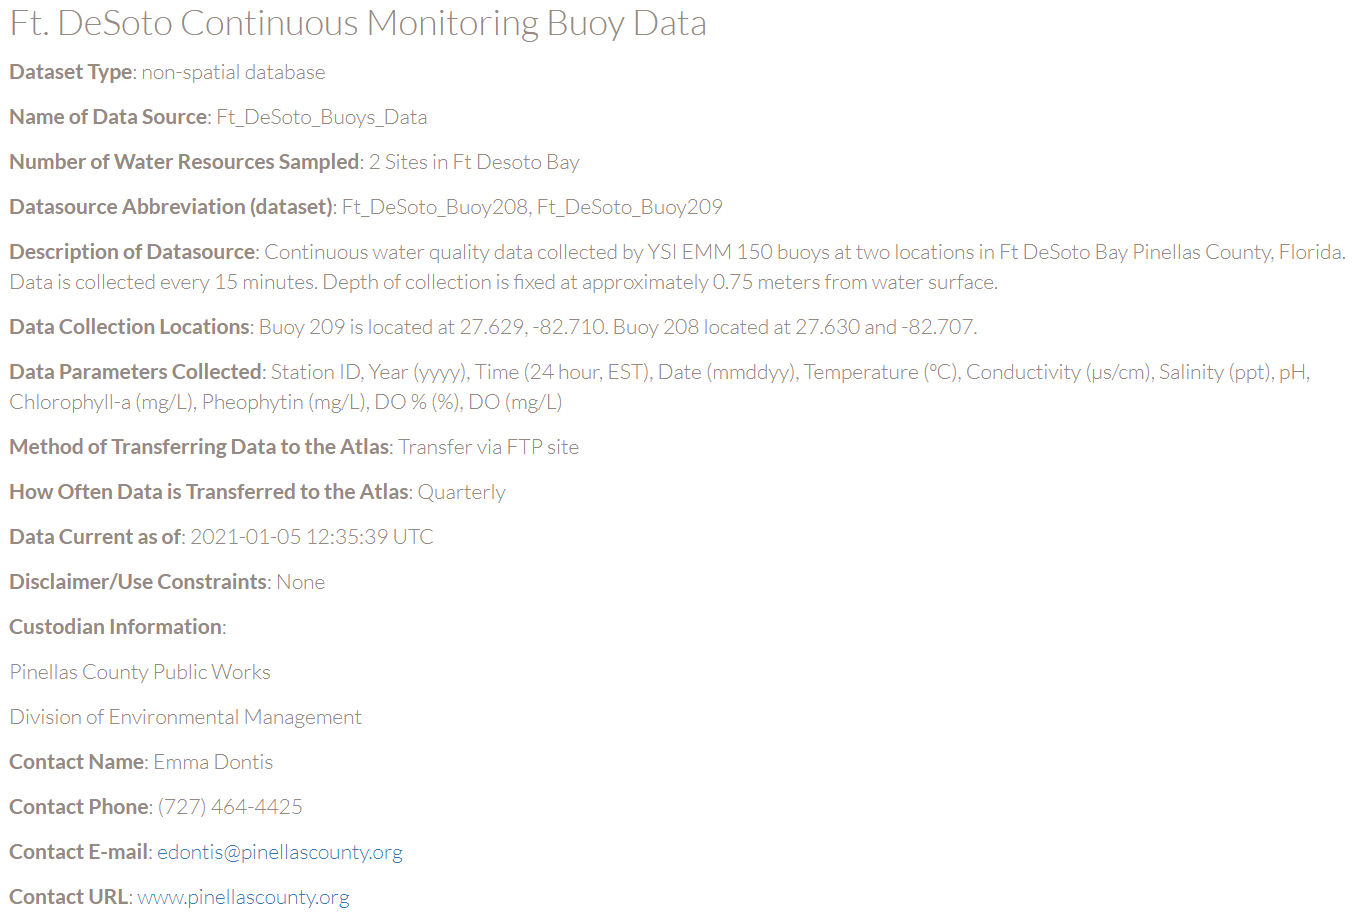
\includegraphics[width=1\linewidth]{img/desotometa} 

}

\caption{A simple example of metadata illustring the principle that something is better than nothing.}\label{fig:desotometa}
\end{figure}

Just by looking at the metadata, we can quickly understand some basic information about this dataset. It describes some water quality monitoring data at two buoys near Ft. DeSoto in Pinellas County, Florida. We can see the type of data, how often it's collected, what equipment was used, the location of the buoys, some contact information should there be questions, and other items that provide additional context. Although it doesn't cover all of the questions above, I would be more than happy to work with these data since this metadata file provides some basic context.

The example in figure \ref{fig:desotometa} represents the bare minimum of what should be done to document metadata. This metadata is an excellent example of the principle that \textbf{some metadata is better than no metadata}. Many datasets lack even the simplest information to facilitate their use by others. At its core, metadata should serve the purpose of providing information about information. No matter the level of specificity or metadata standard that was used, all metadata serve this need. However, more formalized approaches to documenting metadata can play an important role in preparing a dataset for discovery by others and long-term archiving. The next section provides one example of a metadata standard that could be used for environmental datasets.

\hypertarget{eml}{%
\subsection{The EML standard}\label{eml}}

There are countless standards for metadata that go beyond the simple descriptive text shown above. These standards provide a formalized approach or ``schema'' to documenting metadata that provides context about a dataset that is also machine readable. The latter component is critical for making sure that all datasets prepared for hosting or archiving at a data repository follow the same standards for documenting metadata. The core pieces of information (who, what, when, where, why, and how) are included, but in a formalized way to allow for rapid searching and queries when the data are stored along with hundreds to thousands of other datasets.

One such standard that is useful for environmental data is the \href{https://eml.ecoinformatics.org/}{Ecological Metadata Language} or EML. The EML standard defines a comprehensive vocabulary and a readable XML markup syntax (fancy talk for machine readable) for documenting research data. Importantly, the standard is community maintained and developed for environmental researchers who want to openly share their data. The EML standard is also used by the \href{https://knb.ecoinformatics.org/}{Knowledge Network for Biocomplexity} or KNB, which is an online repository that is federated with a much larger network of online data repositories.

The EML metadata file is an XML file that looks something like this:

\begin{figure}

{\centering 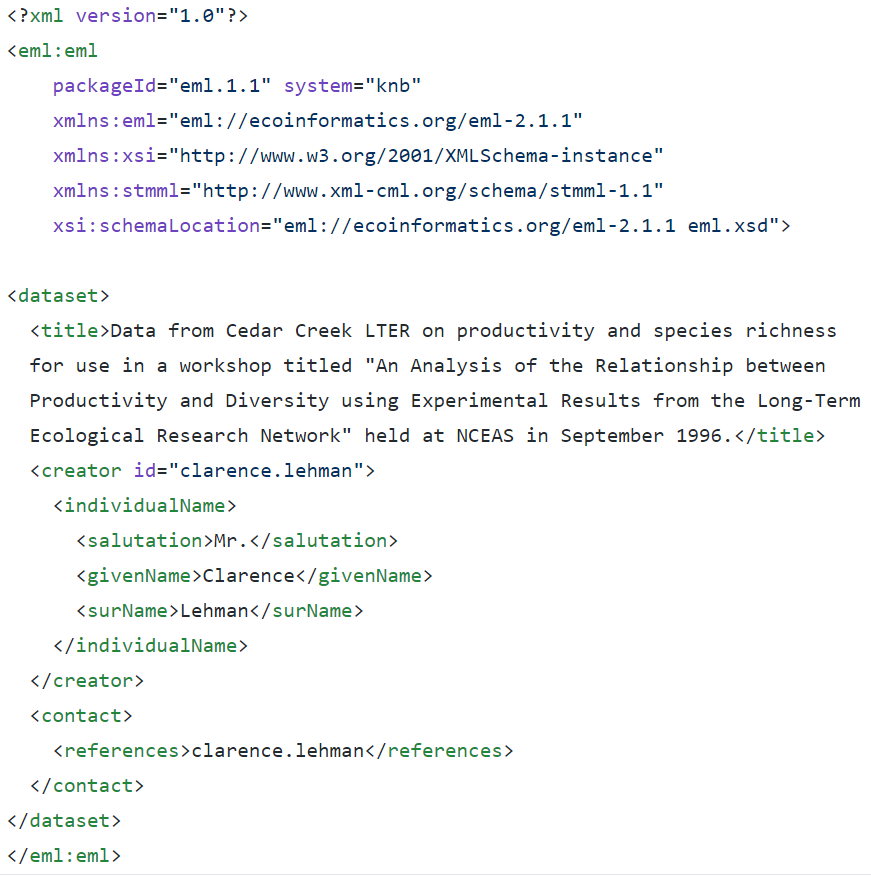
\includegraphics[width=0.7\linewidth]{img/emlsimple} 

}

\caption{A very simple example of an EML file for metadata, shown in XML syntax.}\label{fig:emlsimple}
\end{figure}

The file in figure \ref{fig:emlsimple} might look complicated, but it's just a way to document the basic components of metadata so that a machine can read them. Regarding the descriptive role of metadata, the above example provides a title for the dataset, a brief description, and who to contact. All the rest is additional information about the standard that was used and basic XML tags to identify parts of the document. The EML provides many more standards to document other types of metadata information for the questions in section \ref{metadatadesc}.

A specific reason why EML is mentioned here is the availability of additional software tools to help create EML files for your data. In particular, the \href{https://docs.ropensci.org/EML/}{EML} R package provides these tools to streamline metadata creation. Nobody wants to type an XML file by hand, so the EML packages provides a set of functions where a user can input basic metadata information to create the XML file automatically. All you need is a basic understanding of R and the purpose of metadata to use the EML package for your own needs. More information can be found on the website: \url{https://docs.ropensci.org/EML/}

Of course, you can always manually enter your metadata when you submit a dataset to an online repository. Most repositories, KNB included, provide a form entry system for doing so. An EML file is automatically generated after the metadata have been entered. This may not be the most efficient choice, but is often the preferred for first-timers that may not yet be comfortable using other tools to generate metadata.

\hypertarget{dict}{%
\subsection{Data dictionaries}\label{dict}}

A final note about metadata relates to data dictionaries and what they mean for describing a dataset. A data dictionary is an informal tool for conceptualizing components of a dataset. It is not usually included with metadata, but it's development can inform metadata documentation. This can be incredibly useful for understanding context of a dataset, which is why we include a short description here in the metadata section. However, data dictionaries also have importance for more general best practices for data management. A data dictionary can describe column names and the type of data in each column (Figure \ref{fig:datadict}). Simple things like how you name a data column can have larger implications for downstream analysis pipelines or interpretability of a dataset.

Here we provide some general guidelines for developing your own data dictionary. This is all information that can be included in metadata, but it is also useful to consider for data management.

\begin{quote}
Column names
\end{quote}

Be as descriptive as possible while trying to keep the name as short as possible. Really long names with lots of detail can be just as frustrating as very short names with very little detail. Ideally, the description of data in a column can be included in metadata, but the column name should also be intuitive to point the analyst in the right direction. Try to avoid spaces in column names since some software may interpret that as the start of a new column. It may also be useful to identify a ``plot name'' for each column name \citep{Broman18} that uses proper spelling and punctuation. Using a column name directly in a graphic is generally a bad idea since their meaning outside of the dataset may not be obvious.

\begin{quote}
Column types
\end{quote}

Describe the type of data in each column, e.g., numerical measurements, categorical descriptors, or counts of observations. Never, ever mix data types in the same column. If your data are continuous numeric values, try to identify an acceptable range for the values, e.g., are there minimum or maximum values that would indicate the data are out of range? Also make note of the units that were used. For categorical descriptors, identify all possible categories that are acceptable values for the column, e.g., small, medium, or large for a qualitative descriptor of size. For dates, make note of the format, e.g., YYYY-MM-DD. For time, identify the timezone.

\begin{figure}

{\centering 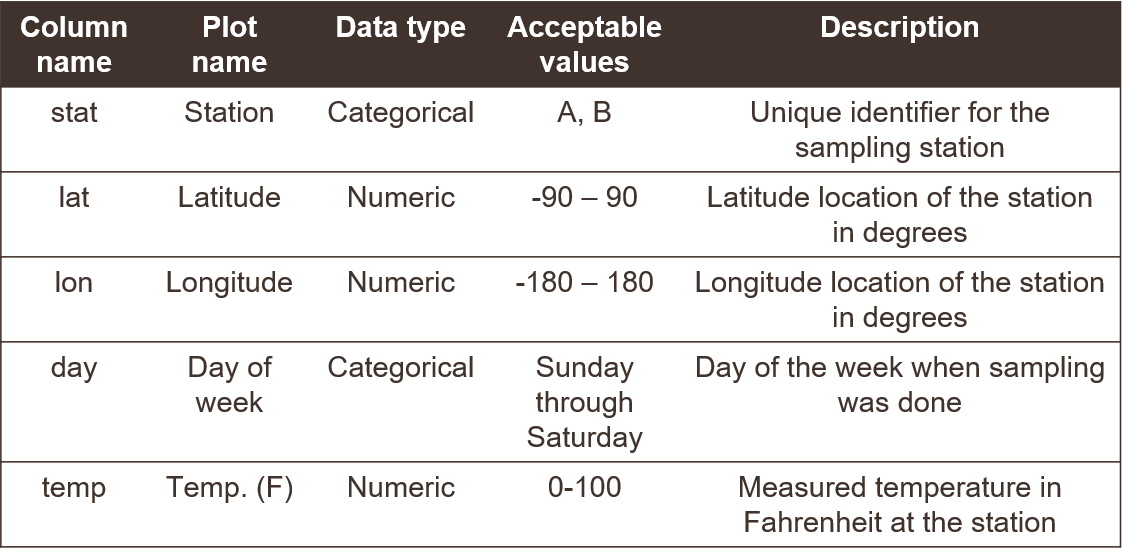
\includegraphics[width=0.8\linewidth]{img/datadict} 

}

\caption{An example of a data dictionary.}\label{fig:datadict}
\end{figure}

\hypertarget{datahome}{%
\section{Where do data live?}\label{datahome}}

Identifying a location for where your data can be stored long-term is an important step in working towards FAIR principles. Hosting your data in an online repository makes your data findable and accessible by others and also ensures that your data are of sufficient quality to adhere to standards for the repository. There is a staggering variety of online repositories, many of which are domain-specific, and it can be difficult to find the best repository that is suitable to your needs.

As with metadata, the same rule applies to online data storage - something is better than nothing. Making your data available in a location that can be accessed by others, including metadata, is much, much better than not sharing your data at all, even if that location is not an ``official'' data repository. For this purpose, online FTP websites can be sufficient. Of course, the major drawback of not hosting your data on an official repository is that others can't easily find the data. You can of course send the link to anyone that's interested, but this means they need to know the data exist to request the link in the first place. A useful scenario is that you include the location of the data as a supplemental link in a published paper or technical report.

Hosting data on \href{https://github.com/}{GitHub} is another simple solution to making your data available to a larger community. GitHub is neither a federated repository, nor is it setup specifically for long-term data storage. However, if you already use GitHub and you want to do something rather rather than nothing at all, GitHub can be a useful solution to begin opening your data. GitHub was initially setup as an online platform for software or code version control, so it doesn't have all the hallmarks of a conventional data repository. GitHub also does not work well with large datasets (e.g., more than 100 Mb). However, it can work well for smaller datasets and offers other amenities that can help you work towards the FAIR principles. For example, the URLs where your data are located are stable (in the sense that they don't change), a DOI can be attached to your data (e.g., through \href{https://zenodo.org/}{Zenodo}), the data are publicly accessible if you choose to make them so, and you can include any appropriate supplemental information (i.e., metadata files). GitHub can be especially useful if your data product is a workflow that includes code to create a tool for environmental decision-making.

A better, but more involved, solution for opening data is using a federated data repository. These are networks of distributed nodes (online access points) or individual repositories that collectively use similar standards in archiving data. They address the problem of multiple disconnected archival systems that are difficult to navigate. For example, the \href{https://knb.ecoinformatics.org/}{KNB} repository is one node of the larger \href{https://www.dataone.org/}{DataONE} federated network. DataONE includes other repositories that are domain-, industry-, or regionally-specific that collectively fall under a more generic category of environmental or earth sciences data. All nodes in the larger DataONE network can be easily navigated and have full infrastructure support from DataONE.

The main advantage of hosting your data in a federated repository is that it will truly be discoverable - it can be found online through standard search queries. No prior knowledge is needed about the data for someone to find the information. For example, perhaps someone is interested in finding datasets within a specific geographic location. They can search the federated network with these criteria and your dataset will be returned if it's within the boundaries. Your metadata includes that information as a queryable attribute. Another advantage is that your data should live on in perpetuity, so long as the internet exists. As mentioned above, GitHub can be a location to store data for open access, however, there is no guarantee that GitHub will always be available as an online service. Federated repositories take great measures to ensure the long-term viability of their resources, including multiple distributed backups in different locations and interoperability of datasets across platforms. You receive those benefits as a guarantee when your data are hosted on these services.

\hypertarget{workflow}{%
\chapter{Data Management Workflow}\label{workflow}}

This section is in two parts to first describe a workflow that we use internally at TBEP to manage our data in section \ref{tbepapproach} and then to describe a road map for opening internal or external datasets at your own organization in section \ref{howyou}. The first section expands on our philosophy for using open science to manage data, including specific workflows we use, as context to the second section. Our approach is one way of applying open science to managing data. Applying the same approach at your organization may or may not be appropriate depending on your internal and external needs for managing data. As such, our approach is generalizable and modular - any of the approaches can be modified in part or together for your own needs.

\hypertarget{tbepapproach}{%
\section{The TBEP approach}\label{tbepapproach}}

\hypertarget{philo}{%
\subsection{Our philosophy}\label{philo}}

Sections \ref{opengeneral} and \ref{philogeneral} introduced you to our basic philosophy and approach to managing data at TBEP. As an organization that facilitates science, management, and outreach activities among our local partners, we adopt open science as a cornerstore strategy that will serve the Program's core values. This approach is made explicit in our \href{https://drive.google.com/file/d/11xohuoaHDxNHRqgXoOHdI37FpWvac_rn/view?usp=sharing}{Strategic Plan} that describes how we achieve programmatic goals defined under our \href{https://indd.adobe.com/view/cf7b3c48-d2b2-4713-921c-c2a0d4466632}{Comprehensive conservation and Management Plan} (CCMP) and who we can work with in our \href{https://drive.google.com/file/d/1iJcWxmc5SeyDTqiCQ3MLQGWEY_EDGtZT/view?usp=sharing}{Interlocal Agreement} to help us achieve our goals.

Our data \href{https://drive.google.com/file/d/1DyA0PNHV8rEXGMwGiyS7sXY1ECLYpJJO/view}{Quality Management Plan} (QMP, \citet{tbep1620}) is a companion document to this SOP that ensures the data used by TBEP for decision-making has known and documented quality and is being used appropriately. The QMP establishes an internal process for verifying data quality standards that conform with federal requirements we have as an organization funded in part by federal dollars under Section 320 of the \href{https://www.epa.gov/laws-regulations/summary-clean-water-act}{Clean Water Act}. On the other hand, this SOP is a more hands-on and accessible document that describes a how-to approach for data management that we adopt as an organization. The SOP goes beyond the QMP by exposing the process and ideas behind how we manage data at TBEP so that others can learn from our experience. We encourage you to also view our QMP to understand the literal benchmark we use to ensure quality of our data.

We actively work to apply open science to every activity we pursue to achieve our goals under the CCMP. Open science is a philosophy and set of tools to make research reproducible and transparent, in addition to having long-term value through effective data preservation and sharing \citep{Beck20}. We use a definition from the \href{https://creativecommons.org/about/program-areas/open-science/}{Creative Commons} for open science as:

\begin{quote}
Practicing science in such a way that others can collaborate and contribute, where research data, lab notes and other research processes are freely available, under terms that enable reuse, redistribution and reproduction of the research and its underlying data and methods
\end{quote}

There are a couple key words from the definition that we can extract - collaborate, contribute, reuse, redistribute, reproduce. These concepts channel some of the ideas described by the FAIR principles (section \ref{fair}). We can further elaborate on these key words by defining open science as a set of four core principles (Dan Gezelter \url{http://openscience.org/what-exactly-is-open-science/}.

\begin{enumerate}
\def\labelenumi{\arabic{enumi}.}
\tightlist
\item
  Transparency in experimental methods, observations, and collection of data.
\item
  Public availability and reusability of scientific data.
\item
  Public accessibility and transparency of scientific communication.
\item
  The use of web-based tools to facilitate scientific collaboration and reproducibility.
\end{enumerate}

Why is this so important? Environmental science is very much in the business of applied science, meaning that research that is conducted to develop an understanding of the environment can be used to support the protection and management of a resource. We need to understand a problem before we can pursue actions to remedy a problem, especially if the wrong decision can be costly. Active and useful channels of communication must exist for the lessons learned from science to be applied to real world problems. Applied science can be facilitated with open science to create these channels.

Without getting too much into the history of how insular practices among academics have contributed to closed science, it's useful to briefly discuss some of reasons why science may not be translated into action. As a generalization, researchers are trained to study and document details. Progress in science is based on 1) an intimate understanding of details that guide process and 2) convincing your peers through rigorous review that you actually understand the details you claim to understand. As a result, we catalog progress in ways that are true to the scientific process, often as dense texts with every last detail noted. Many researchers not being taught otherwise will often assume that this is an effective way to communicate scientific results to non-scientists. What we don't realize is that those that need this information to make decisions do not communicate this way because they are not in the business of scientific discovery. Unless they have a personal interest, they don't care about the science behind the decision, only that the science is right to justify the decision. The most ineffective approach for a scientist to inform environmental management is to deliver a dense 500 page report and assume it provides an effective vehicle for an environmental manager to make a rational decision. This is not applied science - it is ``implied science'' because we implicitly decide that our conventional modes of scientific communication will influence management or policy.

In addition to communication barriers, other challenges to applied science include irreproducible results, information loss, inaccessible data, and opaque workflows (section \ref{whymanage}, Figure \ref{fig:divide}). These challenges affect how science is delivered to decision-makers, how much trust a decision-maker can have in the science behind the decision, and how likely the science can be used as a springboard for more science. Effective data management as a subset of the broader principles of open science can help bridge the ``research-management divide'' and help develop continuity of scientific products that can benefit the larger research community.

\begin{figure}

{\centering 
\includegraphics[width=0.8\linewidth]{img/divide2} 

}

\caption{Challenges to bridging the divide between scientific products created in research and informed decisions for environmental management.}\label{fig:divide}
\end{figure}

\hypertarget{the-open-science-cake}{%
\subsection{The open science cake}\label{the-open-science-cake}}

Truly applied science facilitated by open science allows for research results or data to connect with different audiences along a spectrum. It allows research to be shared with other researchers, be connected with decision-makers, and be accessible to the general public. Where an individual consumes scientific information along the spectrum depends on their interest, need, or level of background knowledge about a subject. A solid technical foundation is a prerequisite for sharing information and open science methods allow various elements of the research foundation to be accessible to different end users. We meet our audience where they're at, rather than assuming they can find their way to the details they need.

We can describe this metaphor as the \textbf{open science cake} (figure \ref{fig:cake}). We use this metaphor because everybody loves cake and it conveniently describes the TBEP philosophy to delivering science in an applied context. This delicious layered cake is a gradient of information from top to bottom. At the top, the information is more general (e.g., educational material for public consumption) or can be used to inform action (e.g., what needs to be done to remedy a problem). At the bottom, the information has specificity and forms the foundation for generality or action at the upper layers. The bottom of the cake is large, reflecting the decades of research and technical resources that are available to inform the management of Tampa Bay (our \href{http://tbep.org/library}{library}, for example). The bottom also includes resources that can be used to springboard additional research, such as analysis code and source datasets. Individuals at the top of the cake probably don't want a slice at the bottom, but the slice they take from the top would not exist without support from the bottom.

\begin{figure}

{\centering 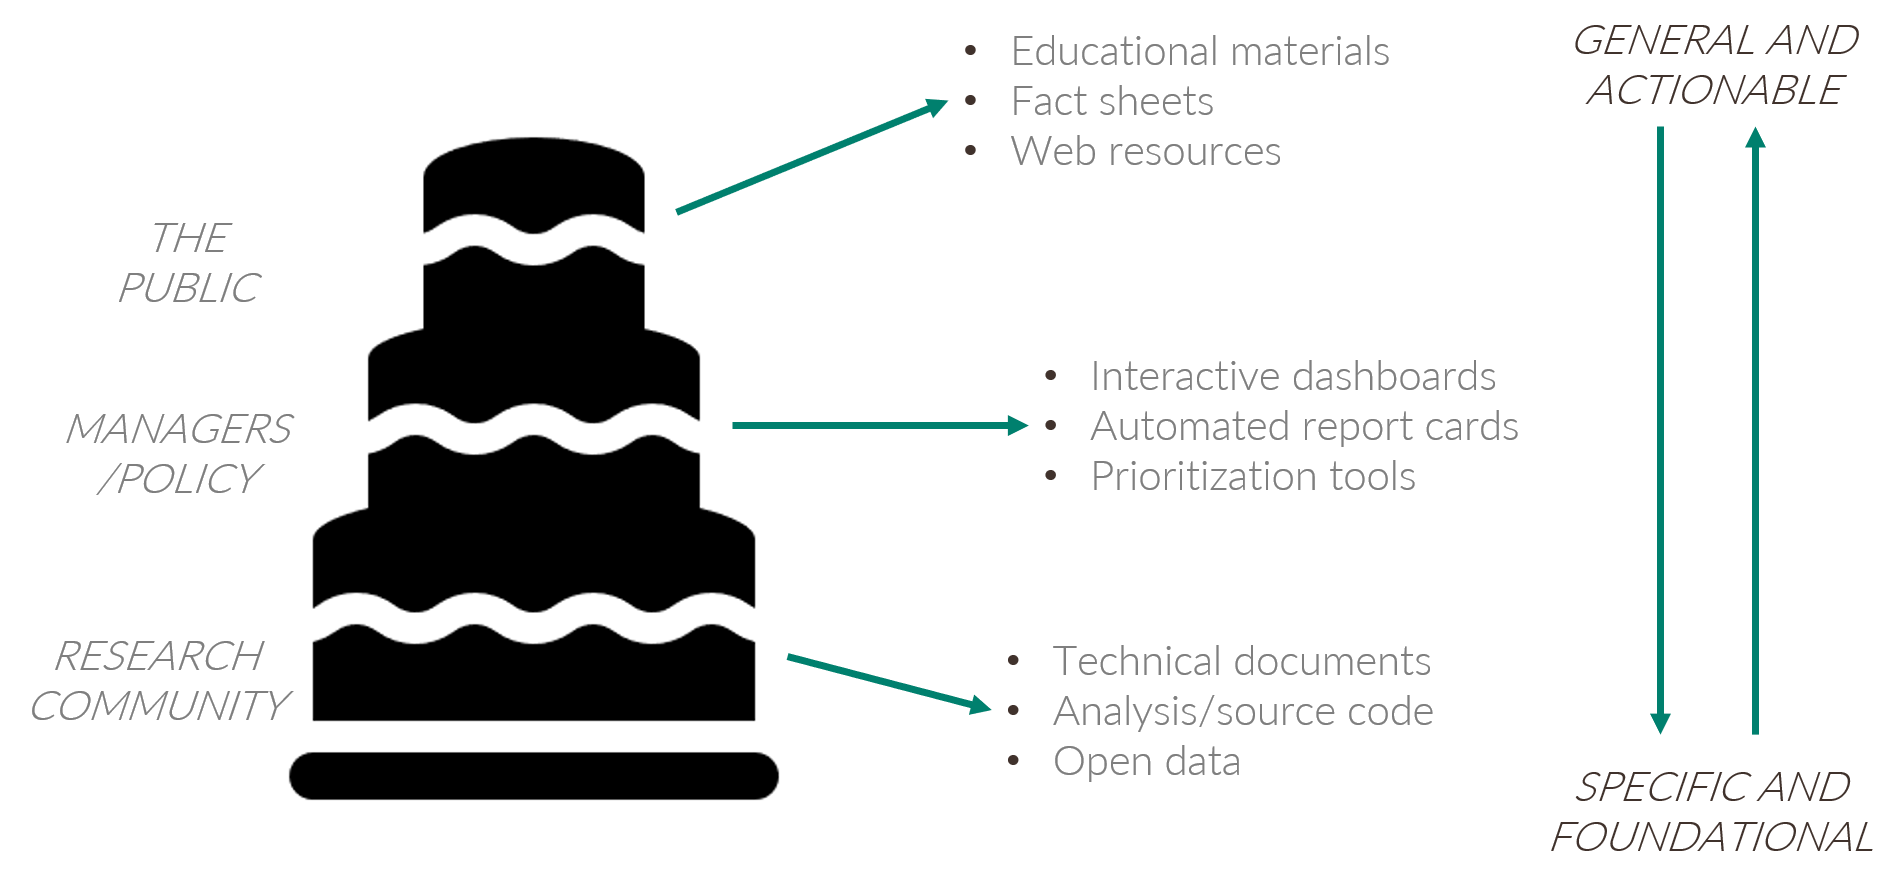
\includegraphics[width=1\linewidth]{img/cake} 

}

\caption{The open science cake showing the connection between research, environmental decisions, and the public.}\label{fig:cake}
\end{figure}

Most of our partners that we work with are professionals from resource management or local government agencies that have some vested interest in the protection and restoration of Tampa Bay. This is our primary audience that we can inform for decision-making. Broadly speaking, this is the audience that needs distilled information from research products but with a level of specificity that goes beyond educational materials. These individuals are in the middle of the cake and the slices they take are actionable science products, such as interactive dashboards, automated report cards, and other decision support tools. The middle part of the cake is where conventional science becomes truly applied science.

The cake also emphasizes a vertical connection among the layers that allows an individual to take a slice as high or as low in the cake as they want. This is a critical principle of open science that speaks to accessibility of information at all levels of the scientific process. Most of the time, an individual will take a slice from the cake at the level that's appropriate for their needs. However, we want our science (and data) to be transparent and accessible under the FAIR principles and someone can take a slice at a different level if they have a need to do so. This also speaks to developing a community of practice for open science - we develop this community to provide easier access to the tools at the bottom of the cake and develop the ability to use them to reproduce or expand on existing products.

Our web products on the \href{https://tbep.org/our-work/data-vizualization/}{data visualization} section of our web page are designed to guide an individual to the slices they need at the different levels of the cake. The website is setup as a series of cards (cakes) for each reporting product that act as an entryway (top of the cake) to the middle and bottom layers of each cake. If someone clicks on the \href{https://tbep.org/water-quality-report-card/}{Water Quality Report Card} for example, they get to a web page that has very general information about the reporting product and links to our \href{https://drive.google.com/file/d/124FXmLcXKYUf3ktaVOvFejndiPS0m7K7/view?usp=sharing}{summary pdf} that distills over forty years of water quality data for the Bay. There are links on the right side of the page that provide access to the building blocks of the report card, including the online dashboard, source code for the report card, build status of the report (more on this in section \ref{automation}), citable DOI, and technical documents that describe the science behind our water quality assessment approach. These links provide the path to the lower levels of the cake.

\hypertarget{automation}{%
\subsection{How do we build the cake?}\label{automation}}

The cake is a useful metaphor to describe how we apply open science to achieve applied science, but how is this done in practice? How are the layers of the cake actually linked to one another? We use several open source programming tools to link source data to reporting products with the goal of producing the most timely information for decision-makers with minimal overhead by internal staff. In this section, we describe these tools and how we link them together to create a workflow that is both automated and reproducible.

The workflow we use to link source data to reporting products for our \href{https://tbep.org/water-quality-report-card/}{annual water quality assessment} is shown in figure \ref{fig:osworkflow}. The process begins by accessing an external data source from our partners. In this case, this workflow accesses a spreadsheet of water quality data on an \href{ftp://ftp.epchc.org/EPC_ERM_FTP/WQM_Reports/}{FTP site} maintained by the Hillsborough County Environmental Protection Commission (EPC). These data are processed using custom-built software developed by TBEP staff and with a suite of more general open source tools, including R, RStudio, relevant data wrangling packages, and tools for document preparation. The open source tools we've created are also hosted online on \href{https://github.com/tbep-tech}{GitHub} which serves two goals. First, providing the tools on GitHub makes them discoverable and accessible to others and second, they are integrated into an automated process to make sure the most current data are used for reporting. Once the build process for the report card is done, the final products as a Shiny web application and our two-page PDF report are hosted on the TBEP website.

\begin{figure}

{\centering 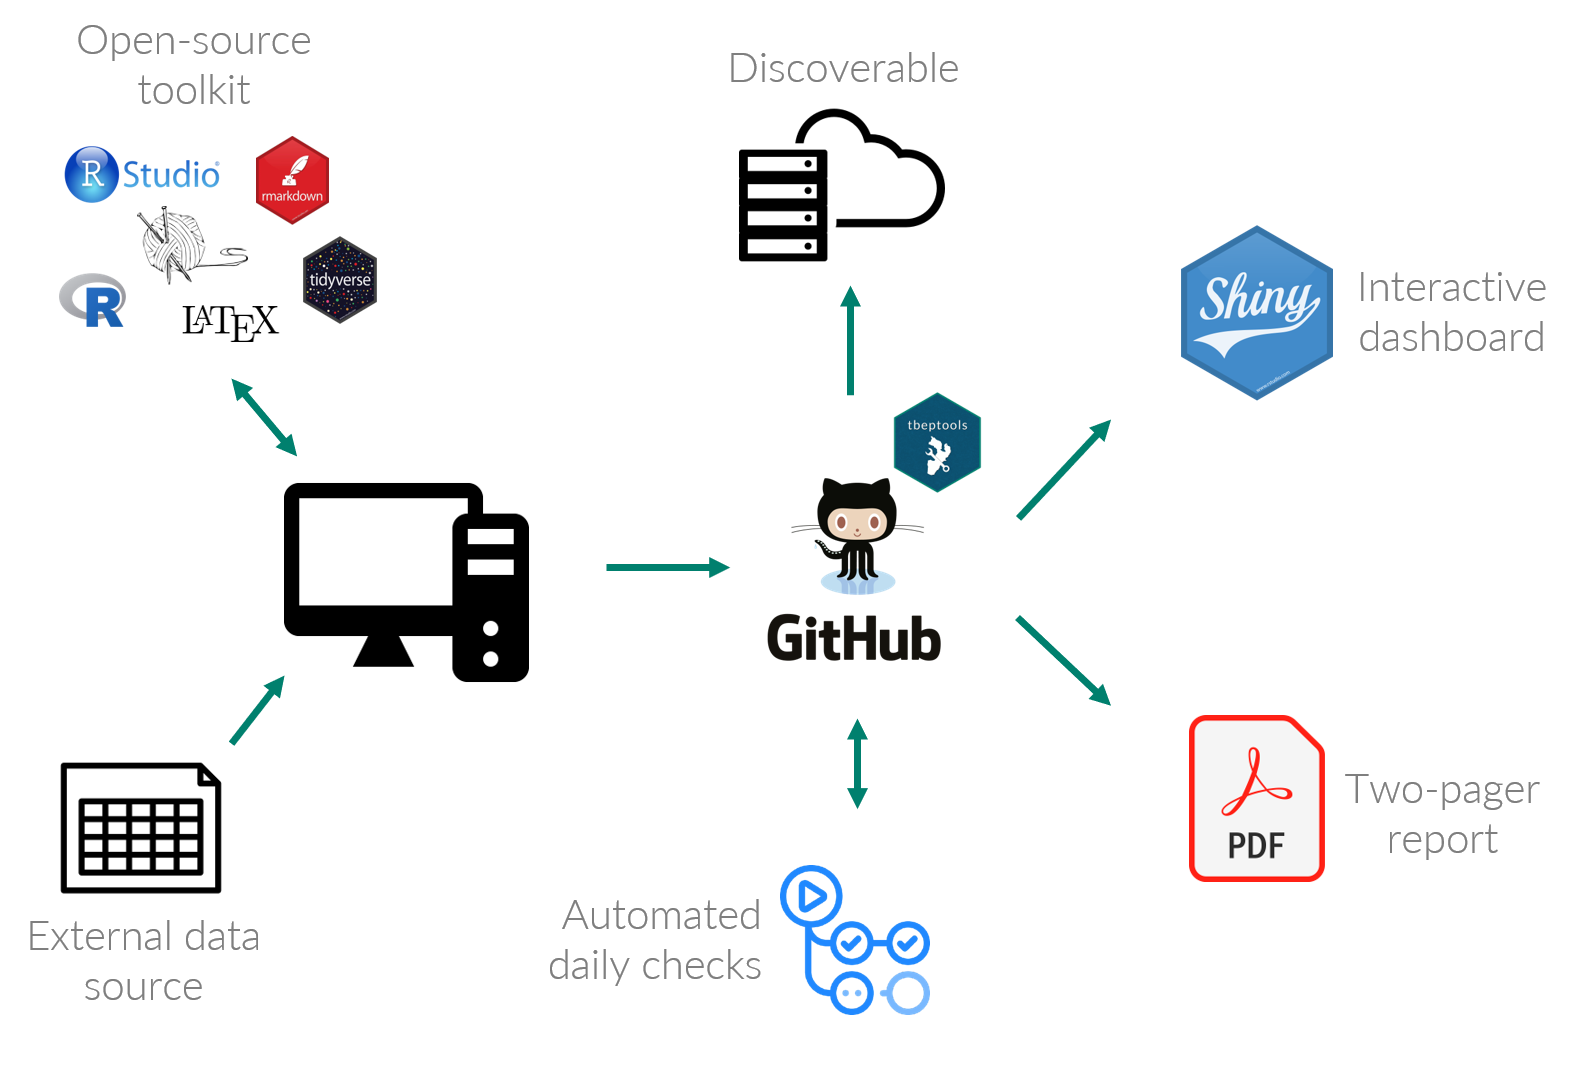
\includegraphics[width=1\linewidth]{img/os-workflow} 

}

\caption{The TBEP open science workflow connecting source data to decision-support tools.}\label{fig:osworkflow}
\end{figure}

The core component of this entire workflow is the \href{https://tbep-tech.github.io/tbeptools/}{tbeptools R package} \citep{Beck21}. This software was developed using the \href{https://cran.r-project.org/}{R programming language} to read, analyze, and visualize data that we use to report on progress in achieving CCMP goals. Most of the data tools on our web page depend on functions within the tbeptools package to work with the raw data provided from our partners. Although tbeptools is primarily used by TBEP staff, the package is provided free of use (under the \href{https://tldrlegal.com/license/mit-license}{MIT license}) for anyone interested in exploring the data on their own. Importantly, all source code is available on GitHub so that anyone with an interest can understand exactly what is done to process the data we use for reporting. This is a very literal definition of method transparency.

There are several functions in the tbeptools package that are built specifically for reporting on water quality, all of which are explained in detail in the \href{https://tbep-tech.github.io/tbeptools/articles/intro.html}{introduction vignette} for the tbeptools package. A ``vignette'' in the R world is a plain language document that explains how to use functions in a package. Currently, the tbeptools package includes five vignettes, one for each indicator that has reporting functions available in the package:

\begin{itemize}
\tightlist
\item
  \href{https://tbep-tech.github.io/tbeptools/articles/intro.html}{Intro to TBEP tools}: A general overview of the package with specific examples of functions for working with the water quality report card
\item
  \href{https://tbep-tech.github.io/tbeptools/articles/tbni.html}{Tampa Bay Nekton Index}: Overview of functions to import, analyze, and plot results for the Tampa Bay Nekton Index
\item
  \href{https://tbep-tech.github.io/tbeptools/articles/tbbi.html}{Tampa Bay Benthic Index}: Overview of functions to import, analyze, and plot results for the Tampa Bay Benthic Index
\item
  \href{https://tbep-tech.github.io/tbeptools/articles/tidalcreeks.html}{Tidal Creeks Assessment}: Overview of functions to import, analyze, and plot results for the assessment of tidal creeks in southwest Florida
\item
  \href{https://tbep-tech.github.io/tbeptools/articles/seagrasstransect.html}{Seagrass Transect Data}: Overview of functions to import, analyze, and plot results for the seagrass transect data collected in Tampa Bay
\end{itemize}

Each vignette is setup similarly by explaining the functions used to read, analyze, and visualize the data. In fact, every function name in the package is named with an appropriate prefix for what it does, e.g., \texttt{read\_transect()} reads seagrass transect data, \texttt{anlz\_transectave()} analyzes annual averages of seagrass frequency occurrence, and \texttt{show\_transect()} shows a plot of the transect data. The examples in the vignette further explain how to use the functions and what each function does when working with the data.

The functions in tbeptools used to read data into R were all built to ensure the most recent data are used for analysis. Each data import function follows a decision tree shown in figure \ref{fig:readchk}, where a set of internal checks are used to see if the data are available on your computer, compare the data to the online source, and download the most recent version if a local file doesn't exist or your current file is out of date. This process also ensures that any downstream reporting products are using the most current data. For example, the web page for \href{https://tbep.org/water-quality-report-card/}{water quality assessment} has a provisional report card that is based on the most recent water quality data available from EPC. Although the ``official'' report card is published at the beginning of each year, provisional data throughout the year can be used to assess water quality changes in near real time.

\begin{figure}

{\centering 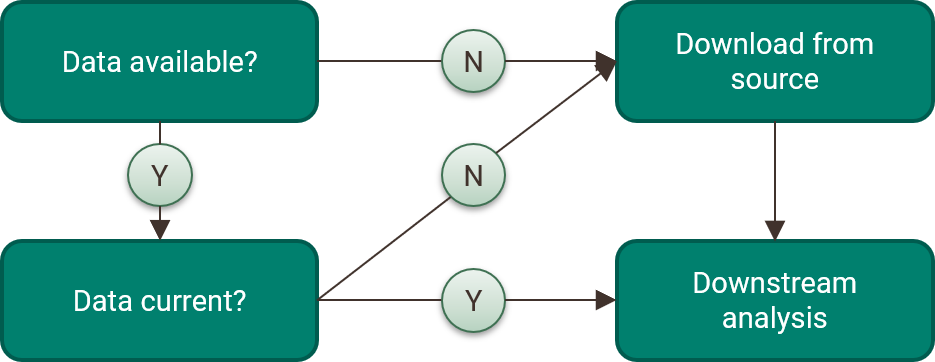
\includegraphics[width=0.8\linewidth]{img/readchk} 

}

\caption{Internal checks used by the tbeptools R package to ensure the most current data are used for analysis.}\label{fig:readchk}
\end{figure}

The workflows we've created that access source data to create reporting products depend on data being online in a stable location. This underlies the importance of proper data management practices. We cannot create and use the reporting products without a findable and accessible location for the source data. The data we use for our various indicators are distributed at different locations depending on who maintains the information. This includes a mix of FTP sites, Microsoft Access databases, JSON files, or geospatial data hosted through third party websites. The various locations, data formats, and depths of available metadata are a potential concern for long-term viability of these workflows. A majority of the locations where these data are found are not formal data archives and there are not any ``official'' standards for how these data are made available. Because of this, a long-term goal for TBEP and our partners is to work towards a shared data management infrastructure that more closely follows the FAIR principles.

A critical part of the workflow in figure \ref{fig:osworkflow} is automation. We have developed the functions in the tbeptools package with this in mind, i.e., making sure the most up to date data are used without having to manually download the data. We also leverage continuous integration/continuous deployment (CI/CD) services through GitHub that automate our workflows. CI/CD simply means that we've setup automated checks and processes based on different triggers that happen when we do something to a project that we've put on GitHub. For example, every time we push (upload) a change that we've made on a local version (i.e., on a personal computer) of tbeptools to the main repository on GitHub, a set of automated checks are used to make sure we didn't break anything in the package. The ``badges'' you see on GitHub and in the data visualization section of the TBEP website indicate if the checks were successful or not. These badges are small indicator icons that are shown as green (checks passing), red (checks failing), or grey (no information). They are often included in GitHub repositories and can also be linked on other websites. These provide a quick scan of whether or not you should expect the package to work as intended if you download it from its current state in the repository.

Many of the README files for the different GitHub projects we maintain include one or more badges that indicate if our data products are working as we hope. For example, the README file for our tbeptools R package includes three badges that indicate the status of different CI/CD processes (figure \ref{fig:badges}). The first badge, R-CMD-Check, shows if the set of standard checks for R packages are passing. There are dozens of checks for R packages, including things like making sure the documentation is up-to-date, file sizes aren't excessive, the file structure is setup correctly, the examples run without errors, etc. (see \href{https://r-pkgs.org/r-cmd-check.html}{chapter 19} in \citet{Wickham15} for a full description of these checks). The second ``pkgdown'' badge shows if the \href{https://tbep-tech.github.io/tbeptools/}{website} for the package (built with the R pkgdown package; \citet{Wickham20}) has been successfully built with the last change to the repository, i.e., does information on the website reflect the package in its current state? Finally, the ``codecov'' badge provides a general estimate of how much code in the package includes unit tests as part of best practices for software development. In this case, nearly all of the code (92\%) is tested in one form or another.

\begin{figure}

{\centering 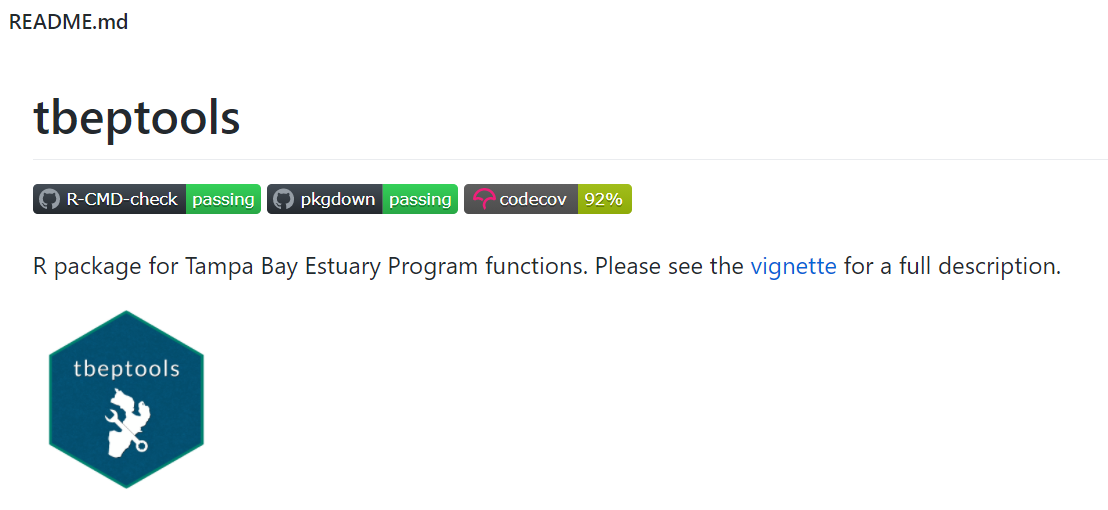
\includegraphics[width=1\linewidth]{img/badges} 

}

\caption{An example of the status badges included in the README file for the tbeptools R package.}\label{fig:badges}
\end{figure}

The CI/CD workflows are completely customizable to suit the needs of a given project. The badges in the previous example simply indicate if the CI/CD checks for a package and its website are working correctly. These are often included in README files to give users peace of mind that our development processes are following accepted standards in the broader open source community. Other badges can indicate if a custom workflow is up to date, such as for our automated reporting products. The water quality report card has a provisional draft that uses the most recent dataset from EPC. The CI/CD process is setup to rebuild the pdf by running a custom ``build'' file that imports the data, analyzes the results, and creates the plots, all using function from tbeptools. The output graphics are embedded in a type of document preparation system that mixes plain text and code to dynamically generate a static pdf. All of this is accomplished in the build file, which is triggered daily through the CI/CD services on GitHub. The CI/CD badge for this repository indicates if the daily build was run and if the provisional pdf was successfully created. Many of our reporting products leverage these services and you can view the status of each product from the badges we've placed on our main TBEP website or on the README file for specific GitHub repositories.

\hypertarget{moregit}{%
\subsection{More on Git and GitHub}\label{moregit}}

GitHub is a foundational tool that is central to our data management workflow. We've described how it can be used as an intermediate solution for hosting data (section \ref{datahome}) and how we use it to share and automate our reporting workflows (section \ref{automation}). Our use of GitHub aligns with our broader philosophy of using open science and here we explain some more general concepts about what GitHub can provide to our community to emphasize the value it can have for data management.

Many people describe Git and GitHub synonymously, but we need to distinguish between the two to develop an understanding of the different services each provides. First, Git is a formal version control software, whereas GitHub is an online platform for sharing code that uses Git. It's possible to use Git without using GitHub (i.e., using version control only on your personal computer) and it's possible to use GitHub without using Git (e.g, using GitHub to share a file). Naturally, using both Git and GitHub together can help leverage the benefits of each. The relationship between the two is very similar to that of R and RStudio. Using R by itself is okay, but the value to yourself and others of using RStudio as a vehicle for R will be greatly enhanced.

Version control is a way to track the development history of a project. It serves joint purposes of 1) formally documenting the changes that have been made to code or software, and 2) making sure that the development history is permanent. Documenting changes provides a transparent record for yourself and others and establishing permanency ensures that any of the changes that are made can be vetted and accessed as needed. Using Git is extra work, but when you need it you'll be glad you've invested your time wisely. Think of an instance where you've saved different versions of a file with different names because you don't want to delete any of your old work. You end up with many extra files and no clear way to understand the origins or connections between the files. Git takes care of this for you by providing a navigable insurance plan for your project.

GitHub lets you share your files or code under Git version control in an online environment so that you and your collaborators can more easily work together. You can host multiple projects under version control, view the entire history of each project, and allow others to more easily work asynchronously and together on the same project. GitHub also has tools for tracking ``issues'' associated with different projects, which provide a simple way to document questions, bug fixes, or enhancements. GitHub is a near perfect example of open source in practice. Anyone can view and potentially contribute to other people's projects using a platform that ensures everything is fully documented and never erased.

GitHub also includes a variety of other tools that facilitate openness:

\begin{itemize}
\tightlist
\item
  Release tagging to assign formal version numbers to code, data or software.
\item
  GitHub actions to create your own CI/CD workflows, our examples in section \ref{automation} use these tools.
\item
  Integration with \href{https://zenodo.org/}{Zenodo} for DOI assignments to give your project a stable and permanent address. You can see these links on many of our projects on GitHub (our \href{https://github.com/tbep-tech/wq-dash}{water quality dashboard}, for example).\\
\item
  Website hosting, as for our \href{https://tbep-tech.github.io/tbeptools/}{tbeptools} R package
\item
  Attaching licenses to a project with visible links to the usages defined under each license
\end{itemize}

All of this may sound very specific to software development, but GitHub can take you a long way towards adopting FAIR principles through better data management practices. The concepts that apply to version control for code and software have parallels for data management and many of the features to facilitate openness in GitHub can also apply to data. Making your data accessible, documenting the changes you've made over time, and establishing a permanent home (e.g., through Zenodo) can all be done with GitHub. We elaborate on a case study example using GitHub for data management in section \ref{twitter}.

GitHub also lowers the barrier to inclusion for engaging others in a project. Unless you work with a dedicated team of software or web developers, it's very rare that your colleagues will have experience with Git or even know what it is (although this may be less common in the future). This doesn't mean that others are excluded from contributing. For example, anyone can post issues for a project through the simple web interface provided by GitHub. Changes to source documents can also be made online that can be tracked through version control without having to use Git on your own (e.g., see our contributing guidelines for this document in section \ref{contrib}).

The TBEP has a \href{https://github.com/tbep-tech}{group GitHub page} where all of our projects exist, including the source content for this SOP. We do this for all of the reasons mentioned above and as an attempt to serve as an example of how open sharing can lead to better science in less time \citep{Lowndes17}. Anyone can view our pages to understand the source code, see the changes we've made over time, and post issues/edit content to directly contribute. This has immense value for how we work as a team and with our partners outside of TBEP.

\hypertarget{howyou}{%
\section{How can you manage data?}\label{howyou}}

This section is written as a road map for managing a data product, keeping in mind the list of tools and resources in section \ref{tbepapproach} that can be used along the way to develop the product. These tools can help you at different stages of the data management process to help build the layers of the open science cake. The guidance provided by \citet{Goodman14} and \citet{Michener15} are also excellent resources presented as ``simple rules'' for working with data. \citet{Goodman14} develops a metaphor of data as a living entity by describing rules for the care and feeding of scientific data. \citet{Michener15} focuses on rules for developing a data management plan. Many of the concepts and tools presented here are elaborated in these two resources.

A road map to developing a plan and set of tools for delivering a data product is shown in figure \ref{fig:dataworkflow}. This map is presented as a hypothetical one-year project from beginning to end, but can be applied to a project of any duration. The steps are separated along a general timeline with a notable distinction between steps occurring before and after data collection. It's also very important to realize that ``data collection'' can have a literal interpretation as collecting data in the field or during an experiment, whereas collection can also be considered generically as the process of creating less conventional data products (e.g., workflows, modelling output/information, decision-support tools, section \ref{contribs}).

\begin{figure}

{\centering 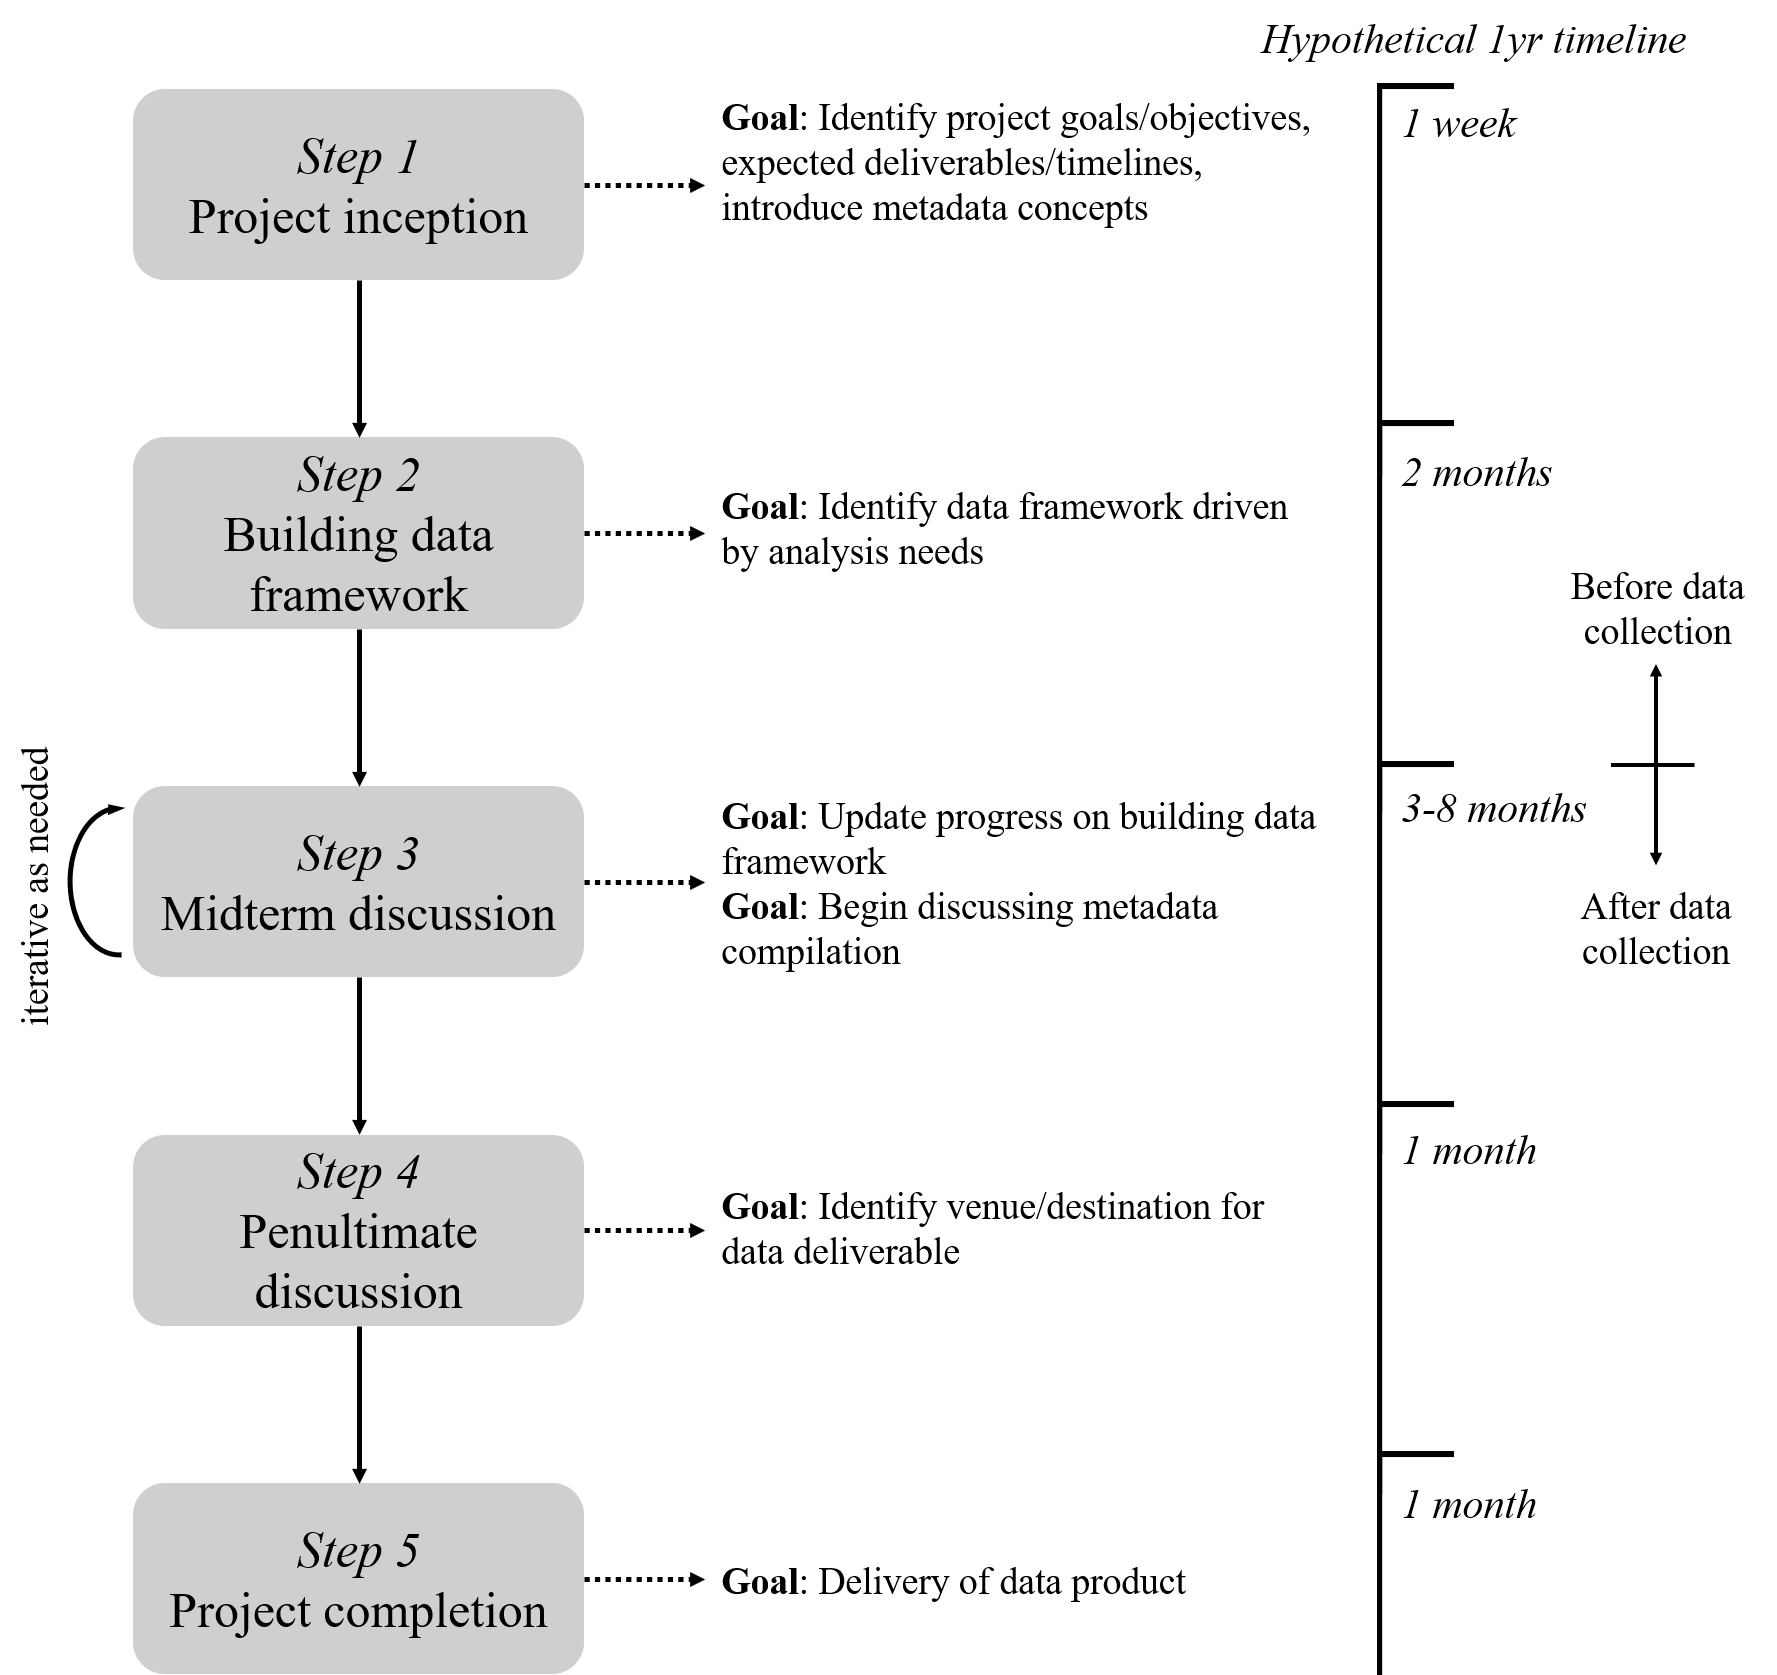
\includegraphics[width=1\linewidth]{img/dataworkflow} 

}

\caption{A hypothetical and generalized timeline for managing data associated with a project.}\label{fig:dataworkflow}
\end{figure}

There are five general steps in the road map. Where you're at in the project determines what conversation you're having with yourself and your research team about managing the data product. At the beginning of a project in Step 1, goals and objectives are defined, potential data contributions are identified, and metadata concepts are introduced. Step 2 is developing the data framework, meaning you will identify how your data are structured within the goals of the project. Here you are thinking about data dictionaries or workflows you will use to generate the data product. In Step 3, you are actively collecting and curating data in a way that conforms to the framework you've developed. This step is iterative because it is where most of the work happens and you may need to rethink some of the ideas around data curation based on how the collection process works in reality. Steps 4 and 5 focus on identifying where the data are going to maintained/stored and finally delivering the data at that location.

The road map in figure \ref{fig:dataworkflow} can be used in parallel with other project timelines, such as those included in a scope of work. It is a separate but complementary approach that focuses specifically on data, as compared to other details associated with a research project (e.g., budget, field work, etc.). The road map also emphasizes that researchers should be proactive in thinking about their data deliverables, particularly regarding important contributions, appropriate formats, and metadata concepts. The earlier these conversations happen in a project, the easier it will be to deliver a well-documented data product.

A researcher or research team will benefit most by using this road map from the inception of a project, although we realize that this may not be the norm and data curation is routinely considered an afterthought. For this reason, we present the following sections as a guide to using this road map at any stage of the research process.

\hypertarget{beginning}{%
\subsection{I'm at the beginning of my project}\label{beginning}}

In an ideal scenario, you are actively thinking about a plan for delivering your data product at the beginning of a research project. Data are the foundation of the project and discussing how you will work with it at the beginning will ensure that the foundation is on solid ground moving forward. Starting the conversation early can also normalize ideas about the importance of paying close attention to data curation. Data are often poorly managed because the value of proper data management to the individual or an organization may not be apparent. These values are also not immediately obvious unless you've spent a lot of time working with other people's data. This includes conversations about the value of metadata. Discussing these details at the beginning of a project will establish a culture of stewardship that is parallel to the larger research process.

Appropriate questions to answer at the beginning and early phases of a project (steps 1 and 2, figure \ref{fig:dataworkflow}) can include the following.

\begin{quote}
What type of project am I working on and what products can I expect?
\end{quote}

The answer to these questions could be based on the intended audience for results that are produced by this research. If your project will have results that can be applied to address some real-world issue, than you are likely working on a project that can deliver a data product to inform decision-making. Think about an appropriate format for this data product that will best meet the needs of your audience.

\begin{quote}
Which datasets are important?
\end{quote}

The answers to the previous questions define your answer to this question. However, it's a rare scenario when you only have one data product as the primary contribution from a project. Early conversations about which data products will be the focus of curation are necessary at this stage. Guidance for determining which datasets are important are expressed in detail in section \ref{contribs}.

\begin{quote}
How do I want to make the data accessible?
\end{quote}

Data typically won't be made accessible until the end of a project, but knowing where your the data will live can help identify what tools you need to use along the way to deliver the product. This includes identifying an appropriate metadata format, analysis platforms to work with the data, and formats that are supported by the location where you're going to keep the data. Having clear answers to these questions will save you the most time at the end of a project.

\begin{quote}
What QA protocols should be established?
\end{quote}

Developing a plan for using the \protect\hyperlink{fair}{FAIR} principles with your data is just as important as ensuring the data have adequate quality for use by you and others. At the beginning of a project, start actively developing a data management plan that defines appropriate methods for collecting the data and verifying its quality. Guidelines in \citet{Michener15} can help with this process or you can use the online \href{https://dmptool.org/}{Data Management Plan tool}.

\hypertarget{middleproject}{%
\subsection{I'm somewhere in the middle of my project}\label{middleproject}}

In a less ideal scenario, you are somewhere in the middle of your project and are just now thinking about types of data products and the path you'll take for their delivery at the end of the project. At this stage, you'll need to retrofit some answers to the questions in the last section to identify important data contributions, how you'll make them accessible, and how you'll collect and format the data to ensure adequate quality. It will be easier to answer these questions if you have yet to collect any data. However, you will need to make sure that you and your research team understands the value of data curation since now it will be seen more as an afterthought that was not discussed at the beginning of the project. You will need to put in some extra work to normalize conversations around data management and why doing so is important.

If you have already collected data, you'll need to take some time to evaluate how you're collecting this information so that it addresses the answers to questions in section \ref{beginning}. If you're collecting tabular data, make sure you are using a tidy data format (section \ref{whytidy}) and that you have developed an appropriate data dictionary (section \ref{dict}) to put some boundaries on how the information is stored. At this stage, it may be impractical and unreasonable to ask field or lab staff to enter their data differently and developing a \emph{post hoc} workflow to wrangle your data into a tidy format may be the best option. Identifying appropriate keys for your data is also critical at this stage. If your data product is more general (e.g., analysis workflow, decision-support tool), make sure you can trace the provenance of these products to their conception. What inputs did you use to create this resource? If you built it from scratch, what tools are you using to build the product (e.g., software and versions)? You may need to do a bit of detective work to identify answers to these questions.

For metadata, the same rules apply in the middle of a project as those at the beginning of a project. First identify where you plan on delivering and hosting your data and work backwards from there. If the location has a specific metadata standard, identify the information you'll need to conform to that standard. If you plan on hosting your data at a more general location, start collecting answers to the ``who'', ``what'', ``when'', ``where'', and ``how'' questions for your data. The most important part of this process is understanding that metadata documentation should start as soon as you realize that you have not been doing so. The longer you wait, the more likely it is that you'll be unable to track down information or you'll simply forget important details about a dataset.

\hypertarget{endproject}{%
\subsection{I'm at the end of my project}\label{endproject}}

Prepare yourself for damage control if you're at the end of your project and have yet to think about data management. You not only have to make some judgment calls on the most important contribution, but you also have to begin the laborious process of finding and extracting intimate details about that contribution. The temptation to identify low-hanging fruit that are easy to document but may not be the most important contribution is very real and you should avoid doing this to not undersell the potential impact of a project. Putting in the time to backlog the provenance of a more important contribution should be an investment that will have more pay off in the future than documenting an intermediate or less relevant data product. The most important question to answer at this stage is what is the most anticipated and impactful result of this research project and what dataset delivers this result?

In the real world, most researchers discuss delivery of a data product at the end of a project because nobody wants to do this at the beginning when more interesting and creative problems about a project are the center of discussion. Of course this is not ideal, but we want to encourage you not to feel overwhelmed and not to give up at this stage. We presented a lot of information about data management so far, but you should not feel that you need to do it all. As before, something is absolutely better than nothing and giving up because you are overwhelmed to do ``all the things'' should not be a deterrent. Open science and data management is incremental and, in reality, very few individuals will be able to complete all of the checklists without years of experience and substantial help from others. So, pick one thing off the list and use that as a starting point to building your comfort and skills in adopting better data management practices (spoiler: it should be metadata).

\hypertarget{metadata-workflow}{%
\subsection{Metadata workflow}\label{metadata-workflow}}

We described general metadata concepts in section \ref{metadata}, but did not provide a workflow for creating or generating metadata. The process begins by answering the general questions we presented as a summary of those in the \href{https://prd-wret.s3.us-west-2.amazonaws.com/assets/palladium/production/atoms/files/Metadata\%20in\%20Plain\%20Language_508compliant.pdf}{Metadata in ``plain language''} document. Just start by writing the answers down in a simple text file or even as a spreadsheet with columns for each question. Where the answers to these questions go depends on how formalized you want to make your metadata, which also depends on where you want to make your data accessible. More informal storage approaches (e.g., GitHub, FTP site) could store metadata as a text file (e.g., in a README document), whereas storing your data in a formal repository would require you to choose an appropriate metadata standard (e.g., EML in section \ref{eml}). Custom workflows that combine metadata documentation through an online user interface can also be created if you or your team have the capacity to do so \citep{Jones07}.

The following can be used as a generalized workflow for metadata generation, ideally at the beginning of a project. How far you go in these steps depends on where you want to store your metadata.

\begin{enumerate}
\def\labelenumi{\arabic{enumi}.}
\tightlist
\item
  Identify which dataset(s) are important contributions of a project that you intend on sharing and that need metadata (see section \ref{contribs}).
\item
  Draft a general document to answer the ``who'', ``what'', ``when'', ``where'', ``why'', and ``how'' questions in section \ref{metadata} for each data product. This can be a simple text file that ``accompanies'' each data product. A spreadsheet entry form can also be useful so that the metadata are in tabular format. If it's tidy, this can be used to import into a program for converting your metadata into a formal standard or for uploading to a data repository.
\item
  Convert the metadata document into an appropriate file format based on the metadata standard you're using. For EML metadata, this would be an XML file.
\end{enumerate}

This workflow is a starting point for creating simple to more complex metadata. For a hypothetical example, the absolute bare minimum for metadata might look this like this (e.g., in a spreadsheet):

\begin{tabular}{l|l}
\hline
Question & Answer\\
\hline
Who & Marcus Beck (fakeaddress@email.com)\\
\hline
What & Water Quality Assessment Data\\
\hline
When & 2020\\
\hline
Where & Tampa Bay\\
\hline
Why & Reporing on annual water quality trends for programmatic update\\
\hline
How & Data were collected monthly as part of the Hillsborough Co. EPC monitoring program\\
\hline
\end{tabular}

If we wanted to add some specificity, we could create separate fields to include more detailed information.

\begin{tabular}{l|l}
\hline
Attribute & Entry\\
\hline
first & Marcus\\
\hline
last & Beck\\
\hline
email & fakeaddress@email.com\\
\hline
title & Water Quality Assessment Data\\
\hline
startdate & 1/1/2020\\
\hline
enddate & 12/31/2020\\
\hline
location & Tampa Bay, FL, USA\\
\hline
west & -82.8\\
\hline
east & -82.3\\
\hline
north & 28\\
\hline
south & 27.4\\
\hline
methods & All data were from the Hillsborough County Environmental Protection Commission (https://www.epchc.org/i-want-to/view-gis-maps-and-data). Data are monthly at mid-depth for each of 50 stations throughout the Bay from 1974 to 2020. Stations were visited on a rotating schedule such that one third of all stations were sampled each week. Bay segments represent management units of interest with distinct chemical and physical differences. Accordingly, station data were aggregated by median values within each of four Bay segments. Data are used to assess progress in achieving programmatic goals for the Tampa Bay Estuary Program.\\
\hline
\end{tabular}

Finally, if we wanted to convert this information to an EML metadata file, we can use some tools in the \href{https://docs.ropensci.org/EML/}{EML R package}. This example includes all of the information from the last example, but using specific tags and entry methods for the EML format, The methods information can also be entered as a separate file for more long-form documentation (i.e., \texttt{set\_methods(\textquotesingle{}data/methods.docx\textquotesingle{})}). After the file is written with \texttt{write\_eml()}, it can be validated for accuracy and completeness with \texttt{eml\_validate()}. The finished metadata file can be viewed \href{data/my_eml.xml}{here}.

\begin{Shaded}
\begin{Highlighting}[]
\KeywordTok{library}\NormalTok{(EML)}

\CommentTok{# enter the metadata}
\NormalTok{me <-}\StringTok{ }\KeywordTok{list}\NormalTok{(}
  \DataTypeTok{individualName =} \KeywordTok{list}\NormalTok{(}\DataTypeTok{givenName =} \StringTok{'Marcus'}\NormalTok{, }\DataTypeTok{surName =} \StringTok{'Beck'}\NormalTok{), }
  \DataTypeTok{electronicMailAddress =} \StringTok{'fakeaddress@email.com'}
\NormalTok{)}
\NormalTok{title <-}\StringTok{ 'Water Quality Assessment Data'}
\NormalTok{coverage <-}\StringTok{ }\KeywordTok{set_coverage}\NormalTok{(}
  \DataTypeTok{begin =} \StringTok{'2020-01-01'}\NormalTok{, }
  \DataTypeTok{end =} \StringTok{'2020-12-31'}\NormalTok{,}
  \DataTypeTok{geographicDescription =} \StringTok{'Tampa Bay, Florida, USA'}\NormalTok{,}
  \DataTypeTok{west =} \FloatTok{-82.8}\NormalTok{, }\DataTypeTok{east =} \FloatTok{-82.3}\NormalTok{, }
  \DataTypeTok{north =} \DecValTok{28}\NormalTok{, }\DataTypeTok{south =} \FloatTok{27.4}\NormalTok{)}
\NormalTok{methods <-}\StringTok{ }\KeywordTok{set_methods}\NormalTok{(}\StringTok{'data/methods.docx'}\NormalTok{)}

\CommentTok{# combine the metadata}
\NormalTok{my_eml <-}\StringTok{ }\NormalTok{eml}\OperatorTok{$}\KeywordTok{eml}\NormalTok{(}
  \DataTypeTok{packageId =}\NormalTok{ uuid}\OperatorTok{::}\KeywordTok{UUIDgenerate}\NormalTok{(),  }
  \DataTypeTok{system =} \StringTok{"uuid"}\NormalTok{,}
  \DataTypeTok{dataset =}\NormalTok{ eml}\OperatorTok{$}\KeywordTok{dataset}\NormalTok{(}
    \DataTypeTok{title =}\NormalTok{ title,}
    \DataTypeTok{creator =}\NormalTok{ me,}
    \DataTypeTok{contact =}\NormalTok{ me,}
    \DataTypeTok{coverage =}\NormalTok{ coverage, }
    \DataTypeTok{methods =}\NormalTok{ methods}
\NormalTok{  )}
\NormalTok{)}

\CommentTok{# write and validate the file}
\KeywordTok{write_eml}\NormalTok{(my_eml, }\StringTok{'data/my_eml.xml'}\NormalTok{)}
\KeywordTok{eml_validate}\NormalTok{(}\StringTok{'data/my_eml.xml'}\NormalTok{)}
\end{Highlighting}
\end{Shaded}

There are many more attributes that can be included in EML metadata. For example, we discussed the importance of a data dictionary in section \ref{dict}. This information can be documented in an EML file in different ways and we encourage you to view the EML \href{https://docs.ropensci.org/EML/}{website} for a full overview.

The intent of presenting this example was to demonstrate simplicity to complexity in the different approaches you can use to create metadata. However, it's also worth pointing out that this process can be completely operationalized through the workflows described in section \ref{automation}. It would be entirely conceivable to use a spreadsheet or web form entry to collect attributes for the EML file, import that information in R, and create the file with the EML R package. This can be automated through a CI/CD build process on GitHub, where a user would only have to enter data on a web form and the rest can be handled through a routine created in R that is executed GitHub. Moving towards this approach to documenting and creating metadata would be a tremendous leap forward in curating data products that are used by TBEP and its partners.

\hypertarget{lets-get-it-online}{%
\subsection{Let's get it online!}\label{lets-get-it-online}}

The previous sections on sharing data have covered general topics on where data could live (section \ref{datahome}) and some options of how we do this at TBEP (section \ref{moregit}). These motivating examples are provided as a set of options that could be used ranging from simple to more complex depending on how detailed and permanent you want to make your data. Your data are less likely to be orphaned the more time you invest in documenting metadata and if you choose a location that is legitimately setup for archiving (e.g., DataOne). The options we presented can be used to achieve these goals with varying success and its up to you which option is most appropriate given the time you have to dedicate to data management and the objectives you have of doing so.

We have not provided step-by-step details on how to deliver a data product online and we leave this exercise up to you. In most cases, getting a dataset online is straightforward but the ease of doing so depends on where you want to put the data. For simple solutions, such as FTP hosting or putting a dataset on Google Drive, all you need to do is upload the data by hand or use an existing file transfer service (e.g., \href{https://www.putty.org/}{PuTTy}). Of course, make sure you also upload any metadata and make it clear that your metadata accompanies the file you uploaded. Hosting data on GitHub can be done using a command line interface (such as Git Bash) or as a GUI through \href{https://desktop.github.com/}{GitHub Desktop}. Tools available in \href{https://happygitwithr.com/rstudio-git-github.html}{RStudio} can also be used to host projects on GitHub.

For more involved hosting platforms, data can also be uploaded through an online web interface. For example, data can be uploaded by hand to the \href{https://knb.ecoinformatics.org/}{knb} node of \href{https://www.dataone.org/}{DataOne} in a web browser, including entry of metadata to generate the EML file. However, open source tools can also be used to link directly to these services to build an integrated data delivery pipeline to avoid uploading information manually. In addition to the \href{https://docs.ropensci.org/EML/}{EML} R package, the \href{https://nceas.github.io/metajam/}{metajam} package can access repositories on DataOne using R. Many of these package are under active development and the services they provide to access federated data repositories is expected to improve over time.

\hypertarget{cases}{%
\chapter{Case Studies}\label{cases}}

In this section we describe three case studies to demonstrate how data management workflows are developed in the wild. In section \ref{automation}, we presented a comprehensive workflow for how we developed our water quality report card. The examples in this section are similar by adopting elements of the previously described workflow, but with some important differences. The examples here represent data products resulting from TBEP and partner-funded research as opposed to a specific reporting product and, more importantly, all of the data management workflows for these projects were developed after the projects were started. This is a no-no for data management, but we provide these examples to demonstrate how we've applied the principles in this document to inopportune but realistic situations. Each example describes the general goals and questions of the project, then outlines the thought process to identifying and documenting important data products.

\hypertarget{oyster}{%
\section{Oyster restoration in Tampa Bay}\label{oyster}}

\begin{figure}

{\centering 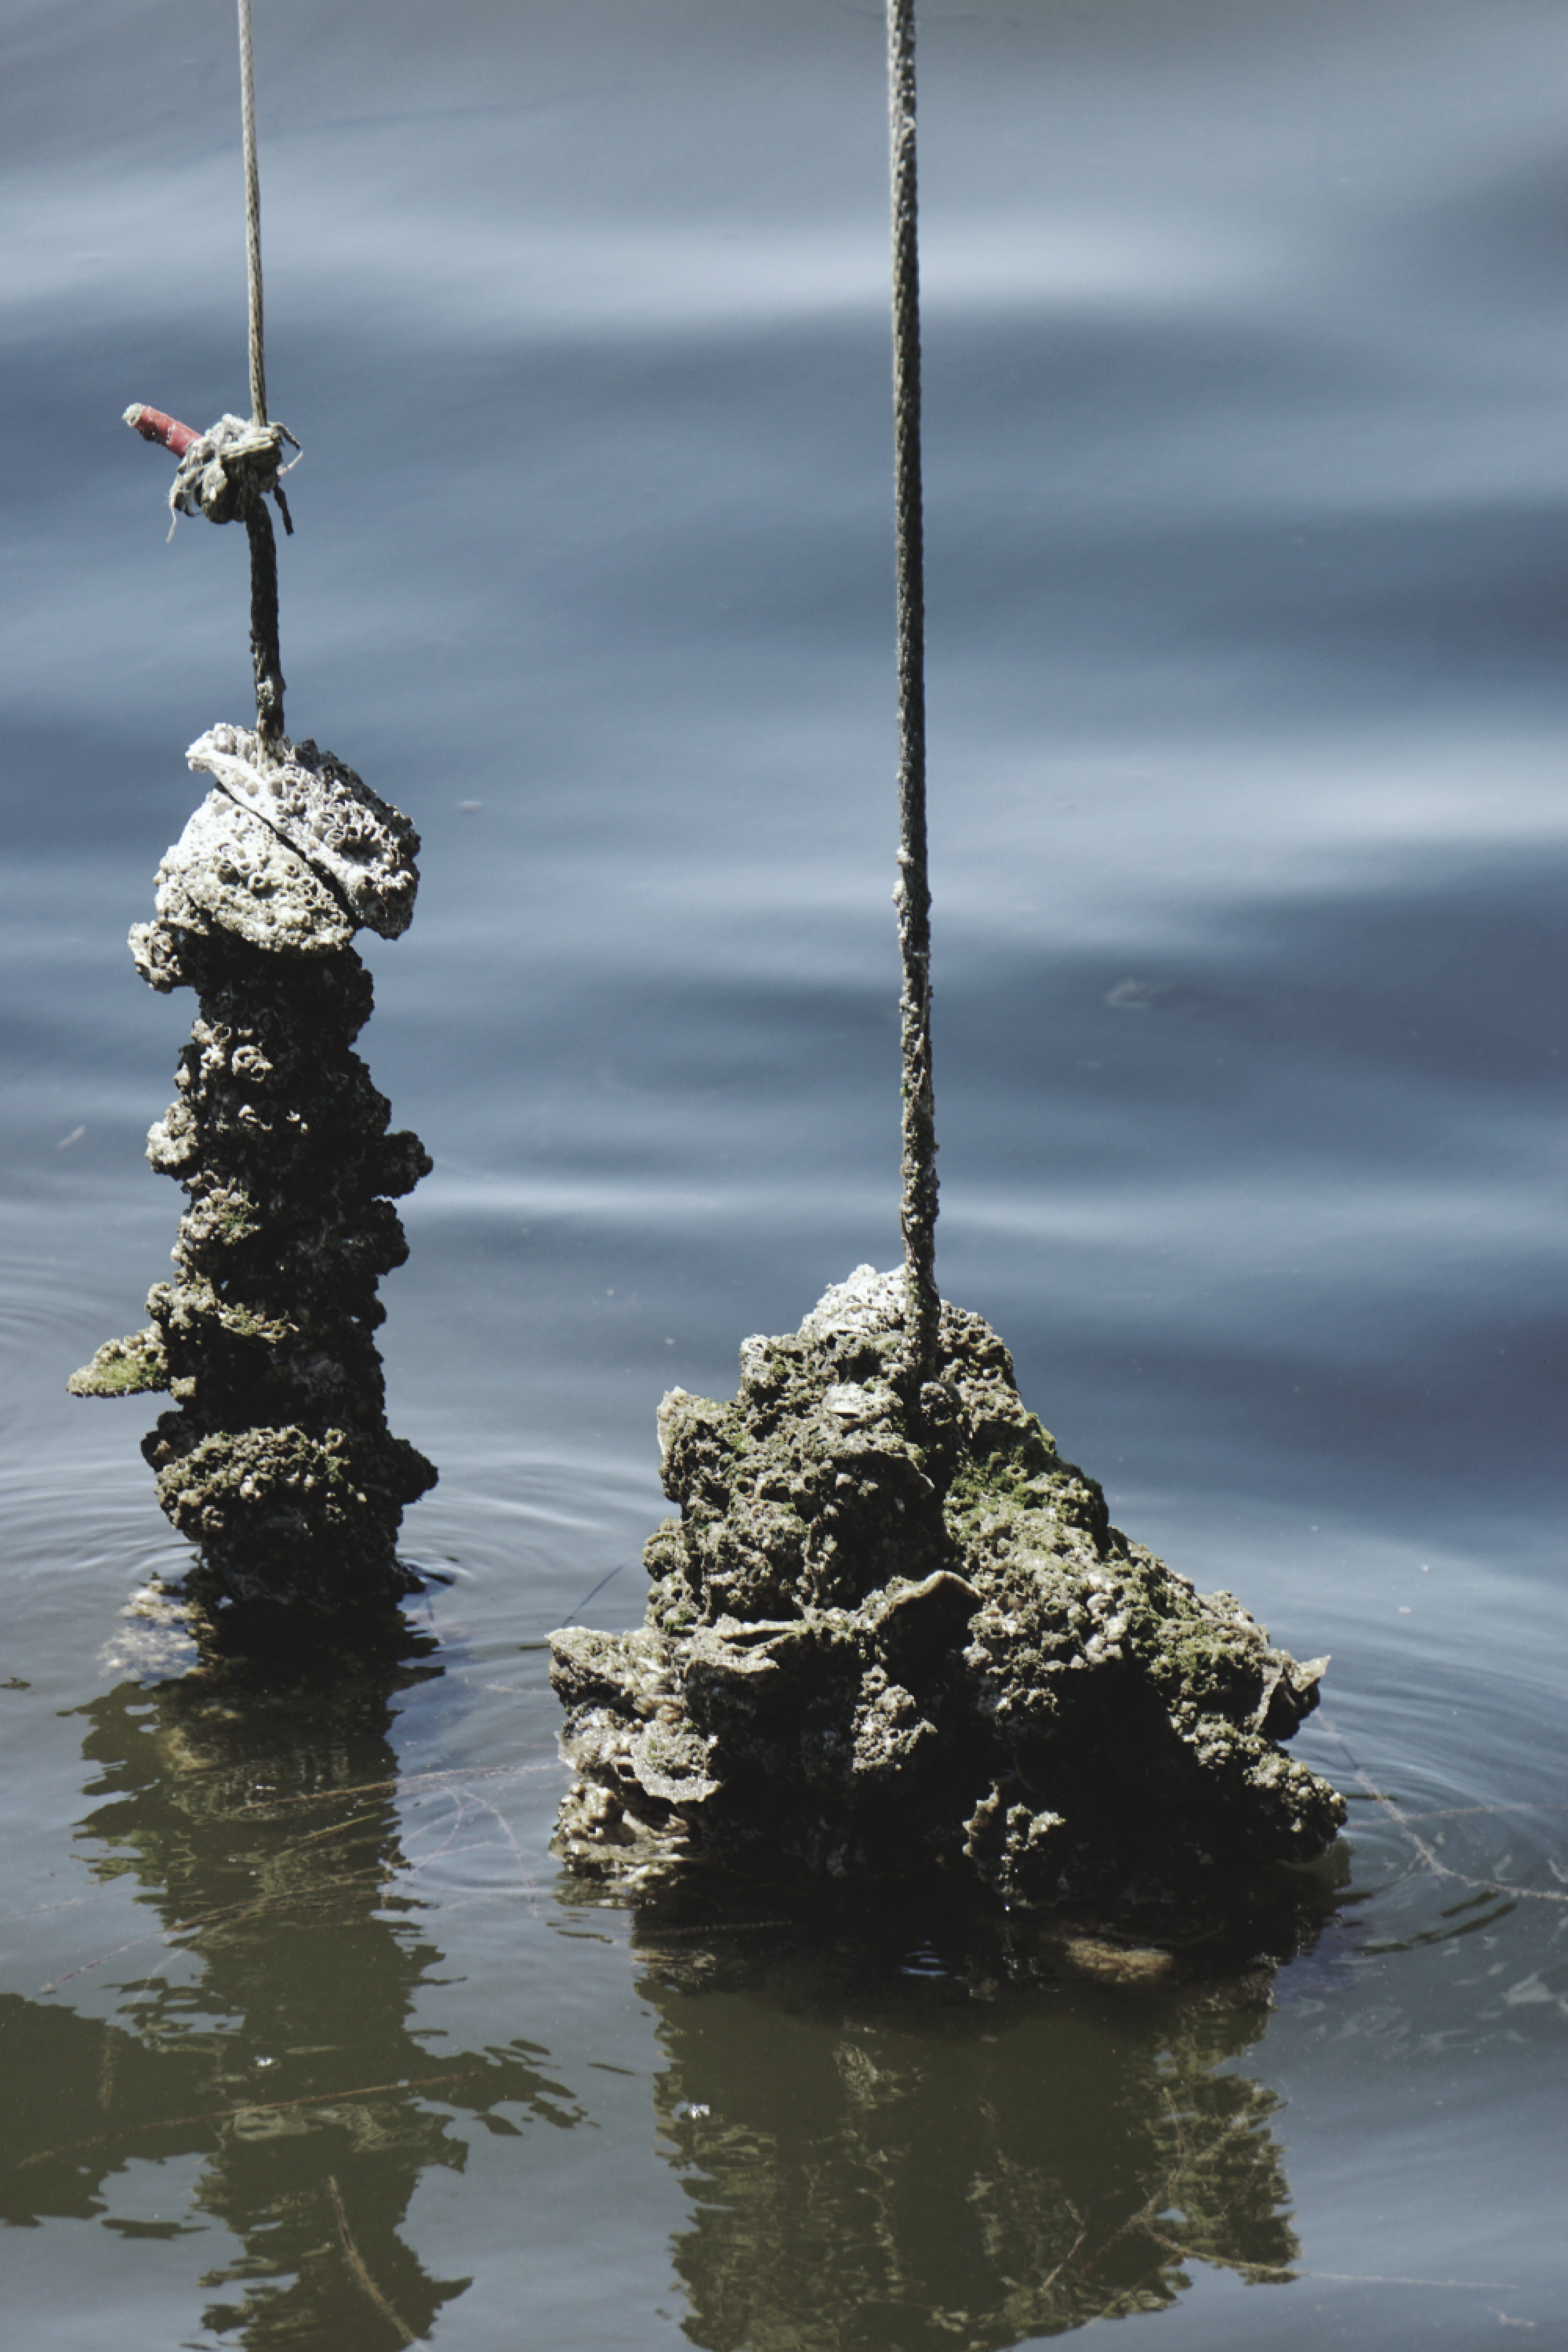
\includegraphics[width=0.5\linewidth]{img/oysters} 

}

\caption{Restoration of oyster reefs (*Crassostrea virginica*) is a critical management goal to support key habitats in Tampa Bay.}\label{fig:unnamed-chunk-11}
\end{figure}

Establishment and restoration of oyster reefs in Tampa Bay is a critical programmatic goal defined under our \href{https://indd.adobe.com/view/cf7b3c48-d2b2-4713-921c-c2a0d4466632}{Comprehensive Conservation and Management Plan} \citep{tbep1017} and \href{https://drive.google.com/file/d/1Hp0l_qtbxp1JxKJoGatdyuANSzQrpL0I/view}{Habitat Master Plan Update} \citep{tbep0720}. Oyster reefs are formed by the cumulative build up of shell material over time and provide food and habitat for other organisms, reduce erosion, stabilize shorelines, and improve water quality. Recreational and commercial harvest of oysters are also important activities that contribute to the value of Tampa Bay. The historical distribution of oyster populations in Tampa Bay is poorly documented, although anecdotal evidence suggests current coverage of oysters Tampa Bay is far less than previously observed. Establishment and restoration of oyster reefs have been fundamental activities to re-establish sustainable populations in the Bay.

Critical questions on factors that contribute to the successful establishment or restoration of oysters in Tampa Bay need to be answered to achieve our programmatic goals. Data have recently been collected to evaluate characteristics that contribute to the long-term success of natural and restored sites, including location in the Bay, seasonal timing of restoration activities, and preferred restoration materials under varying conditions. In addition, standardized monitoring protocols for restoration sites to evaluate or estimate long-term success are needed. This project involves establishing restoration sites at different locations and collecting field data to address relevant questions.

At the time of writing, field data have been collected for the first year of the project and is stored in multiple spreadsheets in an Excel workbook (figure \ref{fig:oysexc}). The field data is a likely candidate for the most important data contribution of this project and a plan for curating these data has recently been developed. This plan is primarily focused on answering questions to identify which factors promote long-term success of oyster reefs, with the intent of formatting the data for analysis to answer these questions and delivering the data in a way to reproduce the results. Environmental managers (e.g., partners that conduct restoration) may have interest in the results (i.e., analysis outcomes), whereas outside researchers may have an interest in using the raw data to support follow-up analysis or to integrate the information with other datasets.

\begin{figure}

{\centering 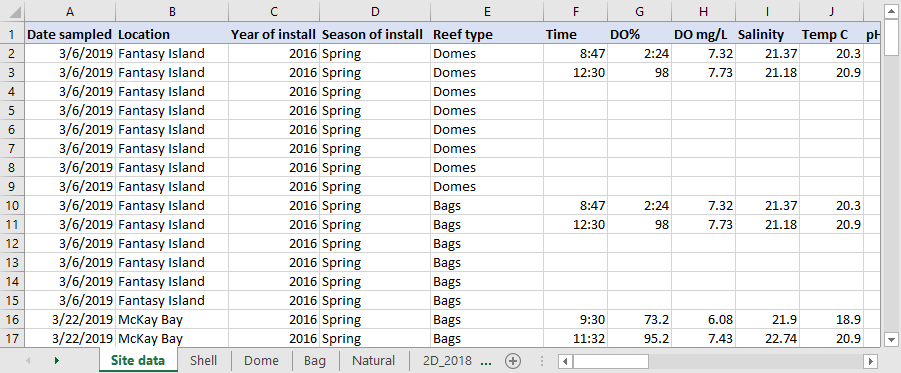
\includegraphics[width=1\linewidth]{img/oysterexcel} 

}

\caption{A screenshot of the raw oyster data from the first year of field work.  The data are close to tidy, but information is spread across tables with no easy way to link between them.}\label{fig:oysexc}
\end{figure}

The current approach for managing these data has focused on adopting a tidy format for the existing information. Because field data collection has already begun, we developed a post-hoc workflow to wrangle the information into flat files with appropriate keys to link data between tables. Identifying a permanent home for these data and formal documentation of metadata have not been done, although tidying the data will aid analysis and facilitate documentation and delivery of final data products. In this example, we focus on the steps to tidy the data.

Our tidying workflow for the first year of field data is available in a GitHub repository: \url{https://github.com/tbep-tech/tberf-oyster}. The raw data are available in the \texttt{data/raw} folder and processing to make them ``tidy'' is accomplished through a custom analysis script at \texttt{R/dat\_proc.R}. The analysis script converts the raw data present in multiple sheets in the Excel workbook to three separate tidy tables. We use functions from the tidyr and dplyr R packages as part of the tidyverse \citep{Wickham19} to format relevant information from the raw data to create the separate tidy tables. This process also involved discussion with project partners when ambiguous labels were observed in the data or presented as conflicting information between tables.

The final ``tidy'' tables include three flat files for the site data (table \ref{tab:tabsitdat}), water quality data at each site (table \ref{tab:tabwqmdat}), and oyster data at each site (table \ref{tab:taboysdat}).

\begin{table}

\caption{\label{tab:tabsitdat}First six rows of the tidy site data.}
\centering
\begin{tabular}[t]{l|l|l|r|l}
\hline
id & site & type & inst\_year & inst\_seas\\
\hline
2D\_bg\_18sp & 2D Island & Bags & 2018 & Spring\\
\hline
2D\_bg\_16fa & 2D Island & Bags & 2016 & Fall\\
\hline
FI\_bg\_16fa & Fantasy Island & Bags & 2016 & Fall\\
\hline
FI\_bg\_08fa & Fantasy Island & Bags & 2008 & Fall\\
\hline
FI\_dm\_16fa & Fantasy Island & Domes & 2016 & Fall\\
\hline
FI\_sh\_05fa & Fantasy Island & Shell & 2005 & Fall\\
\hline
\end{tabular}
\end{table}

\begin{table}

\caption{\label{tab:tabwqmdat}First six rows of the tidy water quality data.}
\centering
\begin{tabular}[t]{l|l|r|r|r|r|r}
\hline
id & date & do\_perc & do\_mgl & sal\_psu & temp\_c & ph\\
\hline
2D\_bg\_16fa & 2019-11-18 & 109.05 & 8.290 & 25.415 & 21.65 & 7.820\\
\hline
2D\_bg\_18sp & 2019-04-02 & 76.45 & 5.870 & 23.235 & 21.70 & 7.815\\
\hline
2D\_bg\_18sp & 2019-11-27 & 93.10 & 7.330 & 24.970 & 19.80 & 7.865\\
\hline
FI\_bg\_08fa & 2019-10-01 & 101.95 & 6.985 & 22.680 & 28.25 & 8.040\\
\hline
FI\_bg\_16fa & 2019-03-06 & 95.05 & 7.525 & 21.275 & 20.60 & 8.095\\
\hline
FI\_dm\_16fa & 2019-03-06 & 95.05 & 7.525 & 21.275 & 20.60 & 8.095\\
\hline
\end{tabular}
\end{table}

\begin{table}

\caption{\label{tab:taboysdat}First six rows of the tidy oyster data.}
\centering
\begin{tabular}[t]{l|l|r|r|r|r|r|r|r}
\hline
id & date & plot & shell\_total & live\_per & spat & aveshell\_mm & maxshell\_mm & aveshell\_cnt\\
\hline
2D\_bg\_16fa & 2019-11-18 & 1 & 75 & 0.9066667 & 0 & 35.480 & 54 & 25\\
\hline
2D\_bg\_16fa & 2019-11-18 & 2 & 99 & 0.9292929 & 0 & 38.000 & 66 & 25\\
\hline
2D\_bg\_16fa & 2019-11-18 & 3 & 39 & 0.7435897 & 0 & 42.960 & 63 & 25\\
\hline
2D\_bg\_16fa & 2019-11-18 & 4 & 181 & 0.8121547 & 20 & 49.920 & 72 & 25\\
\hline
2D\_bg\_16fa & 2019-11-18 & 5 & 77 & 0.8311688 & 0 & 33.160 & 55 & 25\\
\hline
2D\_bg\_16fa & 2019-11-18 & 6 & 23 & 0.6956522 & 0 & 37.375 & 72 & 16\\
\hline
\end{tabular}
\end{table}

Each table is in a tidy format with 1) each variable having its own column, 2) each observation in its own row, and 3) each value having its own cell. The only exception to these rules is the \texttt{id} column which is a combination of site name, restoration type (bags, domes, shell, etc.), installation year, and installation season. This column violates the third rule of tidy data by including multiple values (site name, type, etc.) in one cell. However, the creation of the \texttt{id} column was purposeful to achieve two goals. First, we wanted to create a unique identifier for each restoration site based on our analysis questions of how site location, type, and time of installation influenced restoration success. Each of of these characteristics can be used to evaluate the key research questions for the project. It would be more difficult to compare results between years, if for example, a key that only included site name (e.g., 2D Island only) was used. Thus, it was important to include all identifying characteristics in the \texttt{id} to facilitate the analysis. Second, we wanted the unique identifier to easily convey key information about each site. We could have used a random text string for each unique combination of site, type, installation year, and installation season, but it would be close to impossible to determine relevant details about each site without viewing table \ref{tab:tabsitdat}.

The \texttt{id} keys also allow us to easily join tables for follow-up analysis. For example, we can easily join the oyster data and water quality data for downstream analysis using some R functions from the tidyverse:

\begin{Shaded}
\begin{Highlighting}[]
\NormalTok{combdat <-}\StringTok{ }\KeywordTok{full_join}\NormalTok{(oysdat, wqmdat, }\DataTypeTok{by =} \StringTok{'id'}\NormalTok{)}
\KeywordTok{head}\NormalTok{(combdat)}
\end{Highlighting}
\end{Shaded}

\begin{verbatim}
#> # A tibble: 6 x 15
#>   id         date.x      plot shell_total live_per  spat aveshell_mm maxshell_mm
#>   <chr>      <date>     <dbl>       <dbl>    <dbl> <dbl>       <dbl>       <dbl>
#> 1 2D_bg_16fa 2019-11-18     1          75    0.907     0        35.5          54
#> 2 2D_bg_16fa 2019-11-18     2          99    0.929     0        38            66
#> 3 2D_bg_16fa 2019-11-18     3          39    0.744     0        43.0          63
#> 4 2D_bg_16fa 2019-11-18     4         181    0.812    20        49.9          72
#> 5 2D_bg_16fa 2019-11-18     5          77    0.831     0        33.2          55
#> 6 2D_bg_16fa 2019-11-18     6          23    0.696     0        37.4          72
#> # ... with 7 more variables: aveshell_cnt <int>, date.y <date>, do_perc <dbl>,
#> #   do_mgl <dbl>, sal_psu <dbl>, temp_c <dbl>, ph <dbl>
\end{verbatim}

Storing the data in these three tidy tables reduces redundant information, organizes the data by general categories (e.g., oysters vs water quality), and facilitates follow-up analysis. The GitHub repository also includes an \href{https://tbep-tech.github.io/tberf-oyster/figures.html}{exploratory analysis} of these data created with RMarkdown \citep{Xie18} to combine code and text in an HTML format. This web page is also \href{https://github.com/tbep-tech/tberf-oyster/actions}{built automatically} with GitHub Actions each time the source document is updated (see section \ref{automation}).

In this example, its useful to understand reasons why raw data are often structured in an untidy format. Raw data from field or experimental observations are often setup for ease of entry, whereas tidy data are setup for ease of analysis. Entering data in the field in a tidy format or by hand from field sheets back in the office may seem unnatural. Conceptualizing core components of each dataset and the links between them that can facilitate downstream analyses can be challenging at early stages of a research project. Data wrangling will always be a necessary component of data management, but working towards manual entry in as tidy a format as possible will reduce time preparing the data for analysis or delivery at the end of a project.

\hypertarget{desoto}{%
\section{RESTORE data management: Ft. DeSoto circulation study}\label{desoto}}

\begin{figure}

{\centering 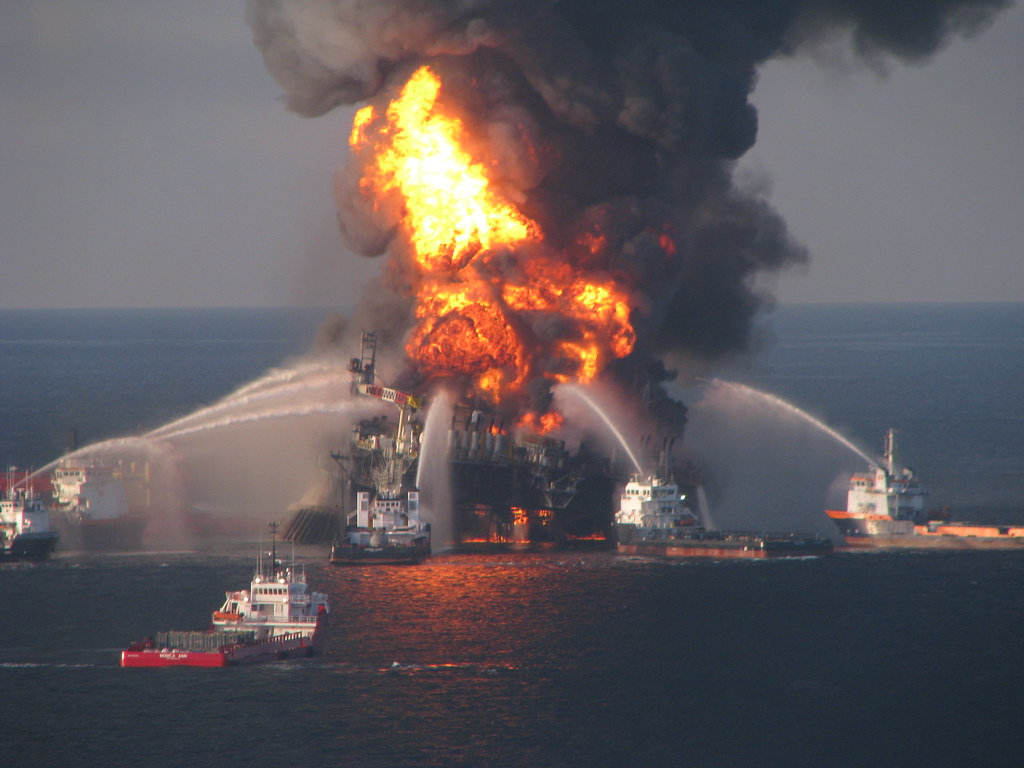
\includegraphics[width=0.7\linewidth]{img/deepwater} 

}

\caption{Billions of dollars were made available for Gulf Coast restoration following legal actions from the BP Deepwater Horizon oil spill.}\label{fig:unnamed-chunk-13}
\end{figure}

The BP Deepwater Horizon oil spill is considered the largest environmental disaster in the history of the petroleum industry. Over 200 million gallons of oil were estimated to have been discharged into the Gulf of Mexico, leading to large-scale environmental damages and economic impacts to Gulf Coast communities. As one of several financial restitutions from responsible parties following this disaster, the federal Resources and Ecosystems Sustainability, Tourist Opportunities and Revived Economies (RESTORE) Act of 2012 established a trust fund to direct billions in US dollars towards expanding ecological restoration on the Gulf Coast.

In partnership with city and county agencies, the TBEP was awarded funds in 2018 under the \href{https://www.restorethegulf.gov/}{RESTORE Council} to advance the protection and restoration of Tampa Bay through projects that address invasive species control, habitat restoration, and climate change. A total of five projects are currently supported under these funds, including 1) facility upgrades at a city of St.~Petersburg landfill, 2) stormwater enhancement at a local park in the city of Tampa, 3) invasive species removal at Cockroach Bay Aquatic Preserve in Hillsborough County, 4) habitat restoration at Robinson Preserve in Manatee County, and 5) habitat restoration, modelling, and monitoring at Ft. DeSoto park in Pinellas County. Each of these projects are ongoing, with RESTORE dollars allowing continuation of activities through the duration of the grant.

A data management plan was drafted at the beginning of the project as a requirement for grant reporting to the RESTORE Council. This plan included text descriptions of anticipated products and associated metadata. The plan also identified internal servers maintained by TBEP as locations for long-term storage of data, made available on request. Although the data management plan begins to develop an approach for curating data products, the location for long-term storage is not accessible nor discoverable outside of our organization. Further, the most important data contributions have yet to be identified and each project is at a different stage of data collection. Developing a unified format for collecting and sharing data from each of these projects will be challenging.

An expansion of the existing data management plan for projects under this grant could benefit from adoption of open science principles and tools to reach a broader audience. As a proof of concept, data products from the Ft. DeSoto monitoring efforts were used as an example for how data delivery workflows could be developed to support and improve data reporting. The Ft. DeSoto portion of this project includes habitat restoration, water quality monitoring, and model development to assess the benefits of bridge openings to improve water circulation in a subembayment of Lower Tampa Bay. A component of the water quality monitoring included deploying two buoys for continuous water quality measurements. These buoys support real-time monitoring of conditions and provide data to parameterize and validate a local hydrodynamic model.

Data curation for the monitoring buoys included several components, all centralized on a \href{https://github.com/tbep-tech/desoto-buoy}{GitHub repository} following a model similar to that in figure \ref{fig:osworkflow}. The data products include the following:

\begin{itemize}
\tightlist
\item
  R Shiny \href{https://github.com/tbep-tech/desoto-buoy}{dashboard} to view and download data from the two buoys (figure \ref{fig:desotoshiny}), including a simple \href{https://shiny.tbep.org/desoto-buoy/\#section-metadata}{metadata} html file (figure \ref{fig:desotometa})
\item
  Full version control with history of \href{https://github.com/tbep-tech/desoto-buoy/commits/master}{changes} made to the repository for hosting the data processing scripts and dashboard
\item
  A permanent \href{https://zenodo.org/record/3941719\#.YFM9069KiUk}{DOI} made available through Zenodo that is linked directly to the GitHub repository
\item
  Automated daily build through \href{https://github.com/tbep-tech/desoto-buoy/actions}{GitHub Actions} that accesses the source data, runs tests, and saves a binary RData file made accessible to the Shiny application
\end{itemize}

\begin{figure}

{\centering 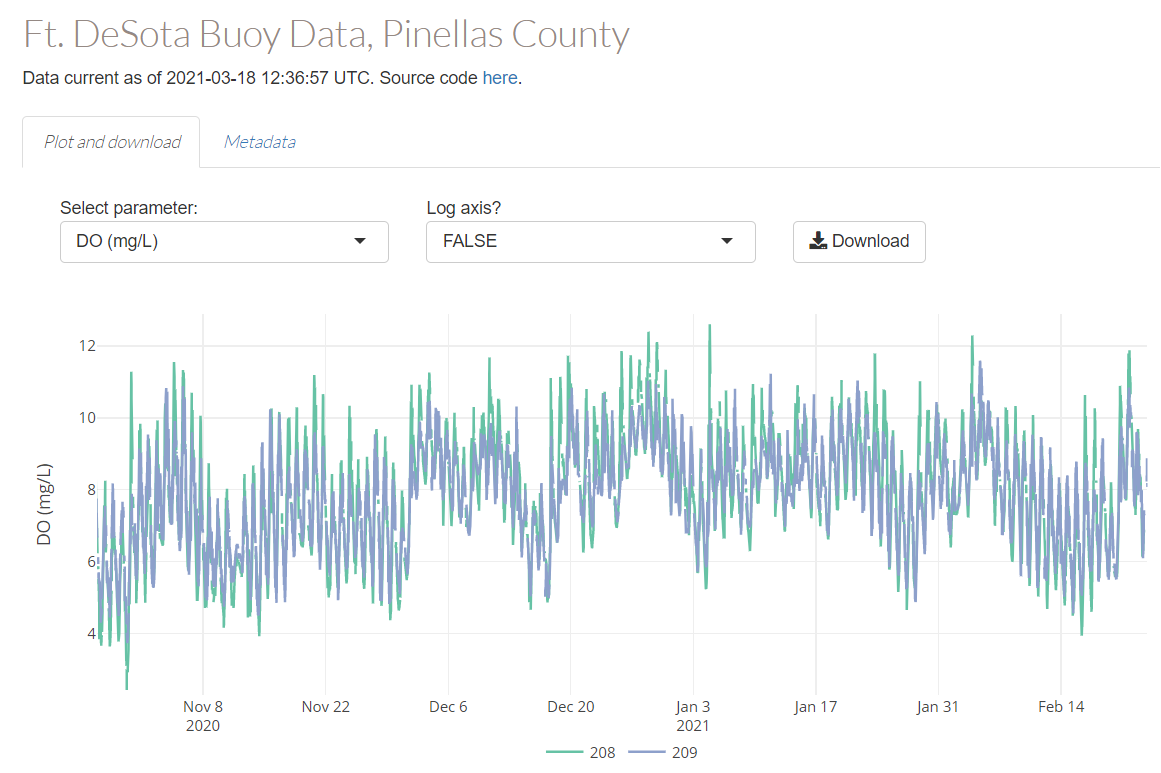
\includegraphics[width=1\linewidth]{img/desotoshiny} 

}

\caption{An R Shiny [dashboard](https://github.com/tbep-tech/desoto-buoy) for viewing and downloading water quality monitoring data for the Ft. DeSoto project.}\label{fig:desotoshiny}
\end{figure}

These products were created with several goals in mind. First, they allow others to reproduce the workflow for alternative applications by exposing the source code for how the data were processed, including metadata as context for the raw data. Second, these products also increase accessibility by providing access to download information from stable locations and allowing interaction for quick visual QA/QC of the data through the dashboard. Third, routine data processing is automated through daily builds and tests that update the information used by the Shiny application by checking the source data on an FTP site. The continuous monitoring data from the buoys are uploaded to the FTP by a satellite connection and a series of tests (using the R \href{https://testthat.r-lib.org/}{testthat} package) are integrated into the daily checks that will create an alert if the processed data do not conform to expectations (i.e., column names change, dates are incorrect, etc.). This service is critical for continuous monitoring data where more information is typically produced by sensors than would be reasonably possible to manually evaluate for QA/QC.

This example is important for demonstrating an expansion of the general concepts presented in section \ref{automation}, where important data contributions are both literal and more general. A literal data product is the dataset produced by the monitoring buoys, whereas the workflow on GitHub for processing the data and hosting the Shiny application is a more general data product. The dataset from the monitoring buoys also has a simple metadata file meant to provide context as opposed to a more formal metadata file that could be used with a standardized data repository. Overall, applying this workflow (version control, Shiny app development, automated tests) is feasible for other important data products created under this grant, but likely impractical for all products. Project managers should carefully consider other important datasets where open science workflows could increase the value beyond simple hosting on internal servers under the existing plan.

\hypertarget{twitter}{%
\section{Red tide and social media}\label{twitter}}

\begin{figure}

{\centering 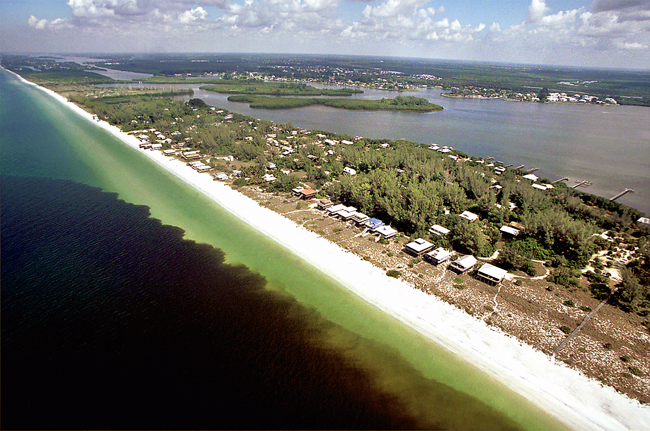
\includegraphics[width=0.8\linewidth]{img/red tide} 

}

\caption{Red tide *Karenia brevis* on the Gulf Coast of Florida (image credit: NOAA)}\label{fig:unnamed-chunk-14}
\end{figure}

Red tides from \emph{Karenia brevis} have been observed on the southwest coast of Florida for over a century. Similar to global trends, these events have increased in severity, frequency, and geographic extent in recent years. Toxins produced by these species and degradation of water quality conditions can negatively impact coastal environments. Large die-off events of marine organisms are commonly observed with red tides, including fish, birds, turtles, and large mammals. Human health during ride tides can be negatively impacted, as toxins are aerosolized out of the water column that can cause respiratory or skin irritation. Tourism or waterfront business revenues are also reduced in areas affected by red tide.

From fall of 2017 to early 2019, one of the longest and most severe red tide events persisted on the southwest coast of Florida for 16 months. Local governments relied on \emph{in situ} monitoring data to respond appropriately to adverse conditions, including identifying areas for clean up or mitigation efforts and issuing local advisories for public health warnings or beach closures. The recent bloom was the first major event since broad public use of social media platforms, offering a unique opportunity to assess complementary sources of information that can aid management response. Twitter is a ``microblogging'' service used by over 330 million people worldwide to share short strings of text or ``tweets'' to convey opinions or ideas on any topic. This project focused on evaluating tweet content, location, and timing as a potential complement for \emph{in situ} data on real-time conditions.

This project was funded through the Tampa Bay Environmental Restoration Fund (\href{https://tbep.org/our-work/restoration-research/tberf/}{TBERF}), which is a grant program in partnership with \href{https://estuaries.org/}{Restore America's Estuaries} that supports priority projects to implement water quality improvement, habitat restoration, applied research, and educational goals of the TBEP and our partners. Data management plans have not been required to secure funding, although recent requests for TBERF proposals as administered by the TBEP have specified a preference for projects that adopt open science approaches for managing data products and deliverables.

The current project was funded in 2019 and is nearing completion. A discussion between project primary investigators and TBEP staff identified a need for delivering data products in an open format, although the data have already been collected and a formal plan for managing these data was not developed at the onset of the project. Identifying important products given the intended audience for project results and how the results could promote additional research were the focus of discussion. This represents a real-world example of how data curation in an open format can proceed at the end of a project, as in section \ref{endproject}.

The Twitter data were used in two analyses, first to characterize links between tweet volume and timing with actual algal bloom conditions, and second, to characterize ``emotional'' content of tweets through sentiment analysis that can inform understanding of public response to natural disasters. Given that this approach has never been used to evaluate social responses to large-scale bloom events, important contributions of the project were the workflow for preparing tweets for the first analysis and custom data products for the second analysis that can be used in follow-up research. In the latter case, this included a ``lexicon'' or vocabulary of emotions that are required for sentiment analysis, but specific to the topic of interest. A time-consuming aspect of sentiment analysis is developing the vocabulary and follow-up research can benefit from having a pre-existing lexicon.

Identifying a location for data products was critical to ensure the results had a lifespan beyond the research paper and that they could have the largest potential impact to inform future management response to red tide. A \href{https://github.com/tbep-tech/red-tide-twitter}{GitHub repository} (figure \ref{fig:redtidereadme}) was created to include supplementary material for the manuscript (in review at the time of writing). The content includes anonymized tweet data (Secure\_Tweets\_data.csv), vocabularies for the sentiment analysis, and R code to run the sentiment analysis. A \href{https://zenodo.org/badge/latestdoi/318579178}{permanent DOI} was also created that linked the repository to the Zenodo archiving service. The repository was listed in the supplementary text for the manuscript to clearly point readers to actual content used for the analysis to facilitate follow-up research.

\begin{figure}

{\centering 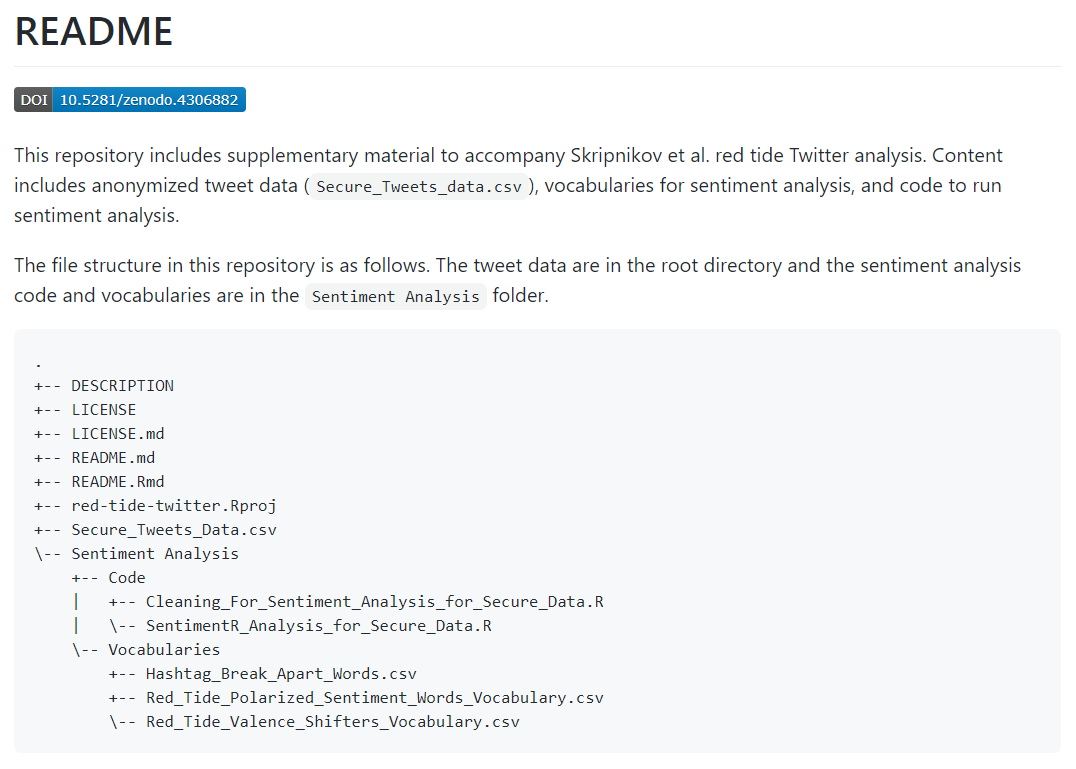
\includegraphics[width=1\linewidth]{img/redtidereadme} 

}

\caption{The README file for the GitHub repository, including relevant data products to evaluate Twitter responses to red tide. Available at <https://github.com/tbep-tech/red-tide-twitter>.}\label{fig:redtidereadme}
\end{figure}

This example is important because it represents the common scenario of identifying an important contribution at the completion of a project. Like the other case studies, the concept of \emph{something is better than nothing} was discussed between the TBEP and project leads. At the completion of the project it was clear that documenting and curating all datasets was impractical and the conversation focused on identifying which components of this work were most important for promoting additional research and informing management actions. Because the application of analysis methods was novel for red tide events, data curation focused on documenting the workflow for tweet analysis and ensuring the lexicon was findable and accessible by others. This was a deliberate attempt to seed additional research on a topic that has not been well-studied.

This project also emphasizes an important point of concern for open data. Tweets include personally identifiable information that can be used to link individuals to user names and geographic locations. Although users consent to use of personal data when they sign up for Twitter, the ethics of using this information for research is a gray area that has no clearly defined rules \citep{Zipper19}. Tweet data can be considered ``passive'' in that they are posted online by users without the intent or knowledge that this information could be used for research. This may suggest that users may reconsider or behave differently if made aware that their data are used for these purposes. In the absence of strict guidance from Twitter, researchers have an obligation to ``self-regulate'' the use of these data by ensuring personal information is cleaned from the data before analysis. The anonymized datasets provided on our repository reflect these principles.

\hypertarget{final}{%
\chapter{Final Words}\label{final}}

This data management SOP is our best attempt at describing a general philosophy of how the TBEP approaches data management and a general framework for how others could manage data at their own institutions. We included a discussion of general and specific topics that are useful to understand for data management (section \ref{keys}), a description of our philosophy towards data management (section \ref{philo}), a general workflow for managing data (section \ref{howyou}), and some case studies demonstrating how these principles play out in the real word (section \ref{cases}). Our approach is constantly evolving as we work towards a more cohesive data plan. The tools described in this SOP will form the foundation of our approach as we figure out what works and what doesn't work for our organization and our partners.

We finish this document by describing some general themes and lessons learned that should serve as useful take home messages about our approach towards data management. Whether you choose to use the specific tools we mention here (e.g., GitHub, R, Shiny, etc.) or adopt other techniques, the themes and lessons present throughout this document still apply. We reiterate them here as a reminder to approach data management with these principles in mind.

\hypertarget{something-is-better-than-nothing}{%
\section{Something is better than nothing}\label{something-is-better-than-nothing}}

Novice data stewards can be overwhelmed by the apparent need to ``check all the boxes'' in the open science workflow of data management. This might include an overwhelming desire to create full metadata documentation using an accepted standard like EML, full version control of data workflows on GitHub, linking a repository with archive services like Zenodo, developing comprehensive data dictionaries, formatting all data in tidy format, and mastering open source data science languages like R. This can be especially daunting when considering that multiple data products could be ``valuable contributions'' of a research project.

Unless you have a fully dedicated IT support team and all the time in the world, it's impractical to try to adopt all of the principles in this document and apply them to every single piece of data for a project. Even applying all of these principles to the single most important data contribution of a project can be impractical. In light of this challenge, the tendency may be to simply treat data in a familiar way using entrenched workflows where data is seen only as a commodity that serves to address the research question at hand. We absolutely encourage you not to fall back on old habits.

Be pragmatic and embrace the idea that \textbf{something is better than nothing} when it comes to data management. Perhaps you set a goal of only checking one data management box for a particular project. Maybe you start by developing a simple metadata text file or developing a data dictionary. Even if you accomplish only one data management related task, this is a vast improvement over doing nothing at all. Channeling this concept, \citet{Wilson17} discuss ``good enough practices'' in scientific computing, acknowledging that very few of us are professionally trained in data science and sometimes ``good enough'' is all we can ask for. So, be kind to yourself when learning new skills and realize that the first step will likely be frustration, but through frustration comes experience. The more comfortable you become in mastering a new task, the more likely you'll be able to attempt additional data management tasks in the future.

\begin{quote}
``Dude, suckin' at something is the first step to being sorta good at something.'' - Jake The Dog, \href{https://en.wikipedia.org/wiki/Adventure_Time}{Adventure Time}
\end{quote}

\hypertarget{just-remember-fair}{%
\section{Just remember FAIR}\label{just-remember-fair}}

We presented the FAIR principles early on in section \ref{fair} as a set of guiding concepts that could be applied to any data management plan. Invoking these principles when managing data can help establish a set of ``goal posts'' to strive to achieve for any data product. If you have questions about whether or not your plan for managing a data product is appropriate, go through each of the FAIR principles to see if they align with your plans. If not, consider an alternative approach or what you can modify in your plan to make them satisfy these principles.

When applying the FAIR principles, there are two considerations to keep in mind. First, we previously mentioned that the principles are purposefully vague as they describe only a general approach to achieving openness. As a result, the principles can have different interpretations to different people. What one data steward considers ``findable'' may not be considered the same by another data steward. This challenge absolutely applies to our descriptions of the tools we described in this SOP. For example, we heavily rely on GitHub in our data management workflows and suggest that serving up data on this platform satisfies the FAIR principles. Others may strongly disagree with this approach because GitHub was developed primarily as a code management platform and not a long-term archive for data storage. This reflects a difference of opinion on what is findable, accessible, interoperable, and reusable, and not to mention, that something is better than nothing.

That being said, the second consideration in applying the FAIR principles is that they also exist on a spectrum and you should not reasonably expect to check all of the boxes to make your data product completely open when first developing a data management plan. You choose what each of the letters mean in FAIR based on your needs or the needs of your organization. Over time, you'll more easily be able to address each of the components of FAIR, but they should be considered guiding principles rather than something that can be rigorously defined.

\hypertarget{the-ever-evolving-toolbox}{%
\section{The ever-evolving toolbox}\label{the-ever-evolving-toolbox}}

The combined wisdom of a larger community of developers to contribute to the development of open source software, such as R, is what makes it so great. The existing tools are visible to others and can be built upon to fix bugs or add enhancements. A much more robust and flexible product is created than proprietary software that is only exposed to a small cabal of developers. However, this benefit is two-sided in that the tools are constantly changing. As tools change, analysis code that once worked may behave differently or not at all. Even more, a relevant skillset may become less useful over time as new methods replace the old.

Any data scientist will admit that a key challenge to maintaining relevance is staying abreast of the constantly evolving toolbox in the open source community. If you choose to incorporate open source software into your data management workflows, consider the potential burden of having to maintain workflows that depend on software under active development by the broader community. This is not an impossible task, but does require a bit of attention on your part to make sure your code is up to date and plays well with others. Making sure you have the most recent software and package versions is a good start. Also avoid incorporating ``professorware'' or other obscure packages into a workflow to reduce the risk of depending on poorly developed tools.

Monitoring various online communication channels can also help you stay abreast of changes in your community. For example, following the \href{https://twitter.com/hashtag/rstats}{\#RStats} hashtag on Twitter can be a good way to monitor the ``conversation'' around existing toolsets. Many of the lead developers actively tweet to announce changes or to solicit input on what could be done to improve software. You can also get a sense of what others are using for specific analyses or workflows. A package that is heavily discussed on Twitter will receive a lot of attention from many users, allowing bugs or features to be more readily addressed. Tracking issues on GitHub for specific packages can also be a good approach to see which changes are taking place or which software packages are actively used by others. An R package on GitHub with very few issues or ``stars'' (similar to ``likes'' on other social media platforms) may be stale or not heavily vetted by the larger community.

It's also entirely possible that broadly used tools like R or Python may no longer be relevant in the not too distant future. The historical evolution of software makes this inevitable. I am 100\% anticipating the day when my skillset, built almost entirely around R, will no longer be relevant because other software platforms and data management workflows have taken its place. When that happens, flexibility and motivation to learn new skills will be critical, even if it means a temporary setback in productivity or efficiency. I have seen this in colleagues that have successfully replaced older analysis platforms (e.g, SAS) with R in their daily workflows. As long as the new tools embrace the broader ethos of open science, it shouldn't matter which platform is the current hot topic.

\hypertarget{look-to-the-community}{%
\section{Look to the community}\label{look-to-the-community}}

Finally, open science embraces the idea that transparent, reproducible, and accessible data products will have the greatest value in a collaborative environment. It's entirely possible to use the tools we describe in this SOP in a completely isolated environment, e.g., developing an R package without sharing, using private GitHub repositories, etc. Unless you use the tools with the intent of engaging and learning from others, then you will never achieve open science bliss.

Interaction with peers is a critical component of the learning process when integrating new tools in a data management workflow. Our mantra above that something is better than nothing indirectly speaks to the need to involve others in this process. It is immensely challenging for a single person to check all of the open science boxes, even for the most skilled data scientists. More than likely, attempts to master all of the tools will spread you thin in other areas of your daily job or even your own expertise as you spend time learning data science skills and not staying up to date on happenings in your field. \citet{Mons18} warns against trying to be both a domain expert and a data expert. A more practical approach to data management is to engage a team with diverse skillsets that not only complement each other, but also can be leveraged as a resource for learning new skills when the time is right.

I close with a graphic from \href{https://twitter.com/allison_horst}{Allison Horst} (figure \ref{fig:codehero}) that skillfully illustrates this concept of using your peers as a support network in learning new tools. Incorporating a new skill into your workflow can be elevated by help from the larger community of software developers, educators, bloggers, mentors, colleagues, and friends. When you hit a road block, look to this community to serve as a safety net to get you out of tricky situations. Your personal success is not achieved in isolation. I would not be where I'm at in my career without the past work of others and the community available at my fingertips through a quick web search. Please keep these resources in mind as you work towards a more FAIR data management plan.

\begin{figure}

{\centering 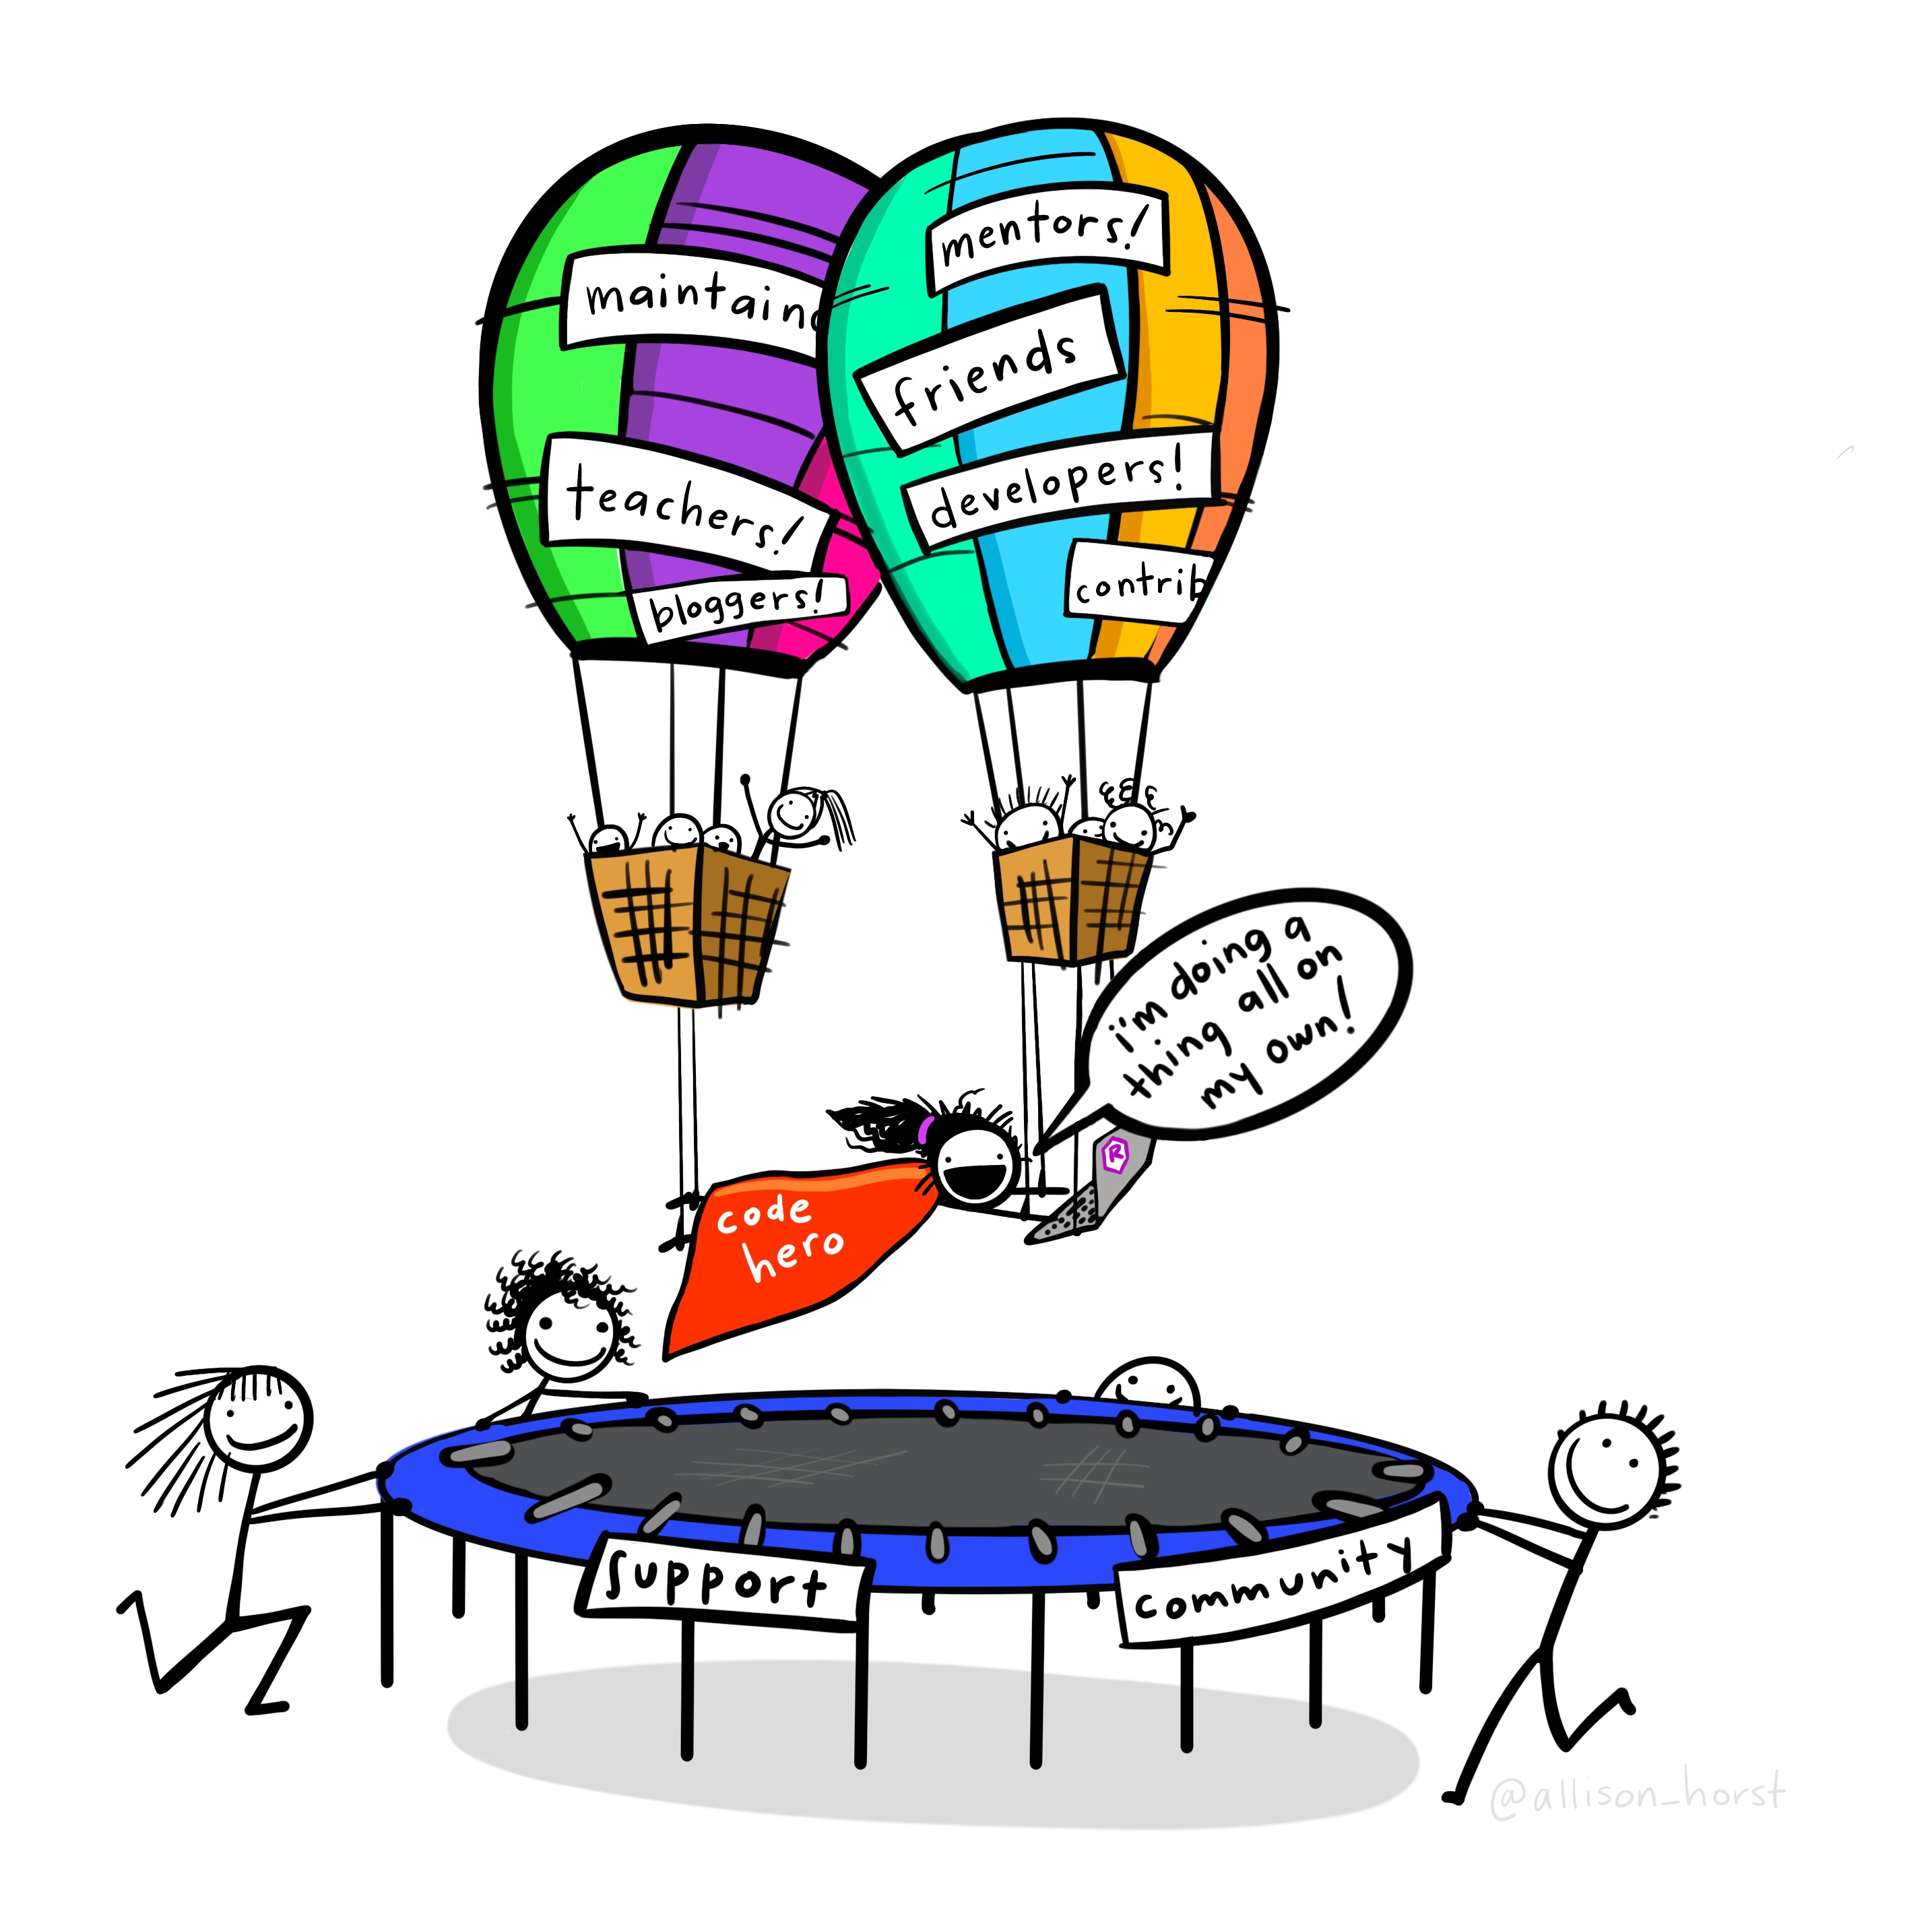
\includegraphics[width=1\linewidth]{img/code_hero} 

}

\caption{Look to the helpers and your open science community! Artwork by Allison Horst.}\label{fig:codehero}
\end{figure}

\hypertarget{appendices}{%
\chapter{Appendices}\label{appendices}}

Below are several resources and definitions that may be helpful in developing a data management plan. This is by no means an exhaustive list. These are resources that we have either curated specifically for TBEP or resources we've found helpful in our own journey.

\hypertarget{list-of-resources}{%
\section{List of resources}\label{list-of-resources}}

\hypertarget{bulding-data-management-plans}{%
\subsection{Bulding Data Management Plans}\label{bulding-data-management-plans}}

\begin{itemize}
\tightlist
\item
  \href{https://environmentaldatainitiative.org/dm-resources/}{Environmental Data Initiative \textbf{Data Management Resources}}
\item
  \href{https://dmptool.org/}{University of California \textbf{DMPTool}}
\item
  \href{https://www.usgs.gov/products/data-and-tools/data-management/metadata-creation}{US Geological Survey resources for \textbf{Metadata Creation}}
\item
  \href{https://ds-wizard.org/}{ELIXIR and others \textbf{Data Stewardship Wizard}}
\end{itemize}

\hypertarget{tbep-r-trainings}{%
\subsection{TBEP R Trainings}\label{tbep-r-trainings}}

\begin{itemize}
\tightlist
\item
  \href{https://tbep-tech.github.io/pep-r-training}{Peconic Estuary Program R training}, \href{https://drive.google.com/file/d/1ZjVHFrVpw2uTKZw-BmD29umdbl6viutM/view?usp=sharing}{recording}
\item
  \href{https://tbep-tech.github.io/ecometab-r-training}{NERRS ecosystem metabolism R training}
  \href{https://tbep-tech.github.io/tbep-r-training/}{TBEP June 2020 R training}, \href{https://www.youtube.com/watch?v=_RI4XMRWeV0\&list=PLfJ6-D-exF9RM5TPtT4T0nxieqpr_R4pJ}{recordings}
\item
  \href{https://tbep-tech.github.io/tbep-r-training/functions.html}{Writing functions in R}
\item
  \href{https://tbep-tech.github.io/tbep-r-training/packages.html}{R package development workflow}
\item
  \href{https://tbep-tech.github.io/tbep-r-training/shiny.html}{A soft introduction to Shiny}
\end{itemize}

\hypertarget{r-lessons-tutorials}{%
\subsection{R Lessons \& Tutorials}\label{r-lessons-tutorials}}

\begin{itemize}
\tightlist
\item
  \href{http://data-lessons.github.io/gapminder-R/}{Software Carpentry: \textbf{R for Reproducible Scientific Analysis}}
\item
  \href{https://datacarpentry.org/geospatial-workshop/}{Data Carpentry: \textbf{Geospatial Workshop}}
\item
  \href{http://www.datacarpentry.org/R-ecology-lesson/}{Data Carpentry: \textbf{R for Data Analysis and Visualization of Ecological Data}}
\item
  \href{http://www.datacarpentry.org/spreadsheet-ecology-lesson/}{Data Carpentry: \textbf{Data Organization in Spreadsheets}}
\item
  \href{https://www.rstudio.com/resources/webinars/}{\textbf{RStudio Webinars}, many topics}
\item
  \href{http://rforcats.net/}{R For Cats: \textbf{Basic introduction site, with cats!}}
\item
  \href{http://www.rstudio.com/resources/cheatsheets/}{Topical cheatsheets from \textbf{RStudio}, also viewed from the help menu}
\item
  \href{http://cran.r-project.org/doc/contrib/Short-refcard.pdf}{Cheatsheet from CRAN of \textbf{base R functions}}
\item
  \href{https://github.com/allisonhorst/stats-illustrations}{Totally awesome \textbf{R-related artwork} by Allison Horst}
\item
  \href{http://www.stat.columbia.edu/~tzheng/files/Rcolor.pdf}{\textbf{Color reference} PDF with text names}, \href{https://www.nceas.ucsb.edu/sites/default/files/2020-04/colorPaletteCheatsheet.pdf}{\textbf{Color cheatsheet} PDF from NCEAS}
\end{itemize}

\hypertarget{r-ebookscourses}{%
\subsection{R eBooks/Courses}\label{r-ebookscourses}}

\begin{itemize}
\tightlist
\item
  \href{http://stat545.com/}{Jenny Bryan's \textbf{Stat545.com}}
\item
  \href{http://r4ds.had.co.nz/}{Garrett Grolemund and Hadley Wickham's \textbf{R For Data Science}}
\item
  \href{https://ismayc.github.io/moderndiver-book/}{Chester Ismay and Albert Y. Kim's \textbf{Modern DiveR}}
\item
  \href{http://tidytextmining.com/}{Julia Silge and David Robinson \textbf{Text Mining with R}}
\item
  \href{http://adv-r.had.co.nz/}{Hadley Wickham's \textbf{Advanced R}}
\item
  \href{https://r4ds.had.co.nz}{Hadley Wickham's \textbf{R for Data Science}}
\item
  \href{https://bookdown.org/yihui/rmarkdown/}{Yihui Xie \textbf{R Markdown: The Definitive Guide}}
\item
  \href{http://www.cookbook-r.com/}{Winston Chang \textbf{R Graphics Cookbook}}
\item
  \href{http://book.ecosens.org/RSEbook/}{Wegman et al.~\textbf{Remote Sensing and GIS for Ecologists: Using Open Source Software}}
\item
  \href{https://geocompr.robinlovelace.net/}{Lovelace et al.~\textbf{Geocomputation with R}}
\item
  \href{https://keen-swartz-3146c4.netlify.app/index.html}{Edszer Pebesma and Roger Bivand \textbf{Spatial Data Science}}
\end{itemize}

\hypertarget{gitgithub}{%
\subsection{Git/Github}\label{gitgithub}}

\begin{itemize}
\tightlist
\item
  \href{http://happygitwithr.com/}{Jenny Bryan's \textbf{Happy Git and Github for the useR}}
\item
  \href{https://ourcodingclub.github.io/2017/02/27/git.html}{Coding Club \textbf{Intro to Github}}
\end{itemize}

\hypertarget{definitions}{%
\section{Definitions}\label{definitions}}

\textbf{CI/CD}: Continuous Integration/Continuous Deployment, describes web services that can be used to automate data checks, tests, or workflows. These are often integrated into existing platforms, such as GitHub Actions on GitHub.

\textbf{Dashboard}: Interactive and dynamic user interfaces available online that can be created to facilitate understanding or to inform decision-making. Many flavors exist, including \href{https://shiny.rstudio.com/}{R Shiny}, \href{https://dash.plotly.com/}{Python Dash}, or \href{https://www.esri.com/en-us/arcgis/products/arcgis-storymaps/overview}{ArcGIS storymaps}.

\textbf{Data}: A general term describing a variety of informational products that can support environmental decision-making or be used to test research hypotheses. Data can be as simple as a single spreadhsheet or more complex products such as model output or parameters.

\textbf{Database}: An organized collection of data, where each piece of data can be linked and accessed electronically through keys that act as unique identifiers for units of information. These are often called relational databases.

\textbf{Data Dictionary}: An informal description of the information included in a dataset, often used to place boundaries on expected values or data types. This includes column names, types of data stored in each column, and expected values for each data type.

\textbf{DOI}: Digital Object Identifier, a unique and permanent name (persistent identifier) for a dataset or other resource, used for archiving and discovery through online queries. Services like \href{https://zenodo.org/}{Zenodo} can be linked to GitHub to create a DOI for a repository.

\textbf{FAIR}: Findable, Accessible, Interoperable, and Reusable, describes general guidelines for creating open data products or assessing the openness of existing products \citep{Wilkinson16}.

\textbf{Flat File}: The simplest form of tabular data, often as a rectangular grid of information stored as \href{https://en.wikipedia.org/wiki/ASCII}{ASCII} text in a non-proprietary file format. There is no information stored in each cell other than the observational values.

\textbf{Keys}: Identifiers that can be used to link data between tables. They are often used to identify unique rows of data, such as a station name or station name/date combination.

\textbf{Federated Repository}: An online network of connected repositories that use similar standards to collectively store data for discovery and access. Uploading a dataset to one node of a repository will make it available through all other nodes.

\textbf{Metadata}: A suite of industry or disciplinary standards as well as additional internal and external documentation and other data necessary for the identification, representation, interoperability, technical management, performance, and use of data contained in an information system \citep{Gilliland16}. Simply put, the who, what, when, where, why, and how of data.

\textbf{Model}: A general term describing a theoretical representation of a real-world phenomenon. It can be as simple as a statistical linear regression model (i.e., y varies as a function of x in a linear fashion) or a more involved mechanistic model with linked equations that describe real-world processes occurring through space and time.

\textbf{Open Science}: A philosophy and set of tools to make research reproducible and transparent, in addition to having long-term value through effective data preservation and sharing \citep{Beck20}.

\textbf{Open Source}: Software with code that is freely available under a license that typically grants users the rights to modify or distribute to others for any purpose. The \href{https://cran.r-project.org/}{R} statistical programming language is one example of open source software used in the environmental sciences.

\textbf{Provenance}: The history of a dataset, including its origin, purpose, and metadata. Formally, this can include the records of inputs, software, and steps of analysis used to create a dataset. The intent is to establish context and also allow reproducibility.

\textbf{Synthesis}: The collection and combination of datasets from different sources, often for research or to inform decision-making. The synthesis product may be considered a novel dataset in itself if the steps in its creation produce novel information not available from its source data.

\textbf{Tidy Data}: A set of simple rules for storing tabular data, including each variable in its own column, each observation in its own row, and each value in its own cell \citep{Wickham14c}

\textbf{Version Control}: A formal software or code development system that tracks and documents changes to create a record that describes the development history and that can be accessed at any time so that previous changes are never lost. \href{https://git-scm.com/}{Git} is version control software, as compared to \href{https://github.com/}{GitHub} which is an online platform for hosting projects using Git.

  \bibliography{refs.bib}

\end{document}
